\documentclass[11pt,a4paper,twoside,openright]{book}
\usepackage{amsmath}
% PAQUETES NECESARIOS
\usepackage[labelsep=period]{caption}
\usepackage{subcaption}
\usepackage{comment}
\usepackage{float}
\usepackage{graphicx}
\usepackage{cancel}
\usepackage[utf8]{inputenc}                 % para poder esribir con acentos
\usepackage[T1]{fontenc}                    % encoding T1 para fonts
\usepackage[english,spanish,es-nodecimaldot]{babel}         % multilenguaje

\usepackage{graphicx}                       % inclusion de figuras 
\usepackage{amsthm, amsmath, amssymb}       % fonts y environments para math
\usepackage{setspace}\onehalfspacing        % espaciado entre lineas
\usepackage[loose,nice]{units}              % units in upright fractions
\usepackage[usarlogouba]{DF-MSc-titlepage}               % titlepage al estilo df.uba.ar
%\usepackage{indentfirst}                    % indentar el inicio de seccion
\usepackage{lipsum}                         % para generar texto generico
%\usepackage{aas_macros}                     % macros para nombre de journals

\usepackage{empheq}                                 %para hacer cajas de texto con color
\usepackage[most]{tcolorbox}

\newtcbox{\mymath}[1][]{%
    nobeforeafter, math upper, tcbox raise base,
    enhanced, colframe=blue!30!black,
    colback=blue!30, boxrule=1pt,
   #1}

\newcommand{\boxedeq}[2]{\begin{empheq}[box={\fboxsep=6pt\fbox}]{equation}\label{#1}#2\end{empheq}}
\newcommand{\coloredeq}[2]{\begin{empheq}[box={\mymath[colback=red!50!black!50!white!50]}]{equation}\label{#1}#2\end{empheq}}


\usepackage{bookmark}                       % para que genere bookmarks en el pdf
\usepackage{fancyhdr}                       % para los headers & footers
\usepackage{emptypage}                      % saca headers and footers de paginas en blanco 
\usepackage{color}
\usepackage{ulem}
\usepackage[margin=1in]{geometry}           % geometria de la pagina 
\usepackage{physics}                        % brakets and such
% CUSTOMIZACIONES PROPIAS
\graphicspath{{./figuras/}}                 % define el directorio de figuras
%\usepackage[Conny]{fncychap}                % para definir estilos de capitulos
%\renewcommand{\vec}[1]{\mathbf{#1}} 	    % vectores como bold
\geometry{bindingoffset=1cm}                % espacio en el borde interno para el encuadernado
\geometry{textwidth=390pt}                  % cuerpo del texto fijo en 390pt
\addto\captionsspanish{\renewcommand{\listtablename}{Índice de tablas}}
\usepackage[svgnames]{xcolor}
\usepackage{hyperref}                       % para vinculos en el pdf
\usepackage{cancel}
\usepackage{bm}
\hypersetup{
    colorlinks=true,
    linkcolor=blue,
    filecolor=magenta,      
    urlcolor=cyan,
    citecolor=Green,
    hyperindex=true,
    pdfauthor={Camila Cristiano},
    pdftitle={Tesis de Licenciatura},
    }

\makeatletter
\def\thickhrulefill{\leavevmode \leaders \hrule height 1ex \hfill \kern \z@}
\def\@makechapterhead#1{%
  %\vspace*{50\p@}%
  \vspace*{10\p@}%
  {\parindent \z@ \centering \reset@font
        \thickhrulefill\quad
        \scshape \@chapapp{} \thechapter
        \quad \thickhrulefill
        \par\nobreak
        \vspace*{10\p@}%
        \interlinepenalty\@M
        \hrule
        \vspace*{10\p@}%
        \Huge \bfseries #1\par\nobreak
        \par
        \vspace*{10\p@}%
        \hrule
    \vskip 40\p@
    %\vskip 100\p@
  }}
\def\@makeschapterhead#1{%
  %\vspace*{50\p@}%
  \vspace*{10\p@}%
  {\parindent \z@ \centering \reset@font
        \thickhrulefill
        \par\nobreak
        \vspace*{10\p@}%
        \interlinepenalty\@M
        \hrule
        \vspace*{10\p@}%
        \Huge \bfseries #1\par\nobreak
        \par
        \vspace*{10\p@}%
        \hrule
    \vskip 40\p@
    %\vskip 100\p@
  }}
\DeclareMathOperator*{\mcm}{mcm}

\titulo{Entrelazamiento y fase geometrica en un modelo de Jaynes-Cummings disipativo de dos atomos}
\subtitulo{}
\autor{Ali Martin Zynda Aiub}
\numerodelibreta{342/20}
\lugardetrabajo{Departamento de Física, FCEN, UBA}
\director{Dr. Fernando Lombardo}
\codirector{Dra. Paula Villar}
\fechadeinicio{Marzo de 2024}
\fechadefinalizacion{Marzo de 2024}
\fechadeexamen{18 de diciembre de 2024}



\begin{document}

% Organizacion del manuscrito
%
% Frontmatter
    %\frontmatter
%   Titlepage
    \maketitle
%   Dedication
   \newenvironment{dedicacion}%
{\thispagestyle{empty} \cleardoublepage\null \thispagestyle{empty} \vfill\begin{center}% 
\textbf{} \end{center}}%
{\thispagestyle{empty} \vfill\null }

%\pagestyle{empty}
%\null\vspace{\stretch{1}} 
\begin{dedicacion}
\textit{}



\end{dedicacion}
%{\it
%
%
% 
%}
%\end{flushright}
\vspace{\stretch{2}}\null
%   Resumen (en espanol e ingles)
    \frontmatter
    \spanishlcroman
    \cleardoublepage
\pagenumbering{roman}
\setcounter{page}{1}
%\setcounter{tocdepth}{2}
\tableofcontents

    \listoffigures
    \newenvironment{abstract}%
{\thispagestyle{empty} \cleardoublepage\null \thispagestyle{empty} \vfill\begin{center}
\bfseries \abstractname \end{center} }%
{\thispagestyle{empty} \vfill\null }


\selectlanguage{spanish}
\begin{abstract}


\end{abstract}

%\selectlanguage{english}
%\begin{abstract}



%\end{abstract}
\selectlanguage{spanish}




    \newenvironment{agradecimientos}%
{\thispagestyle{empty} \cleardoublepage\null \thispagestyle{empty} \vfill\begin{center}% 
\textbf{Agradecimientos} \end{center}}%
{\thispagestyle{empty} \vfill\null }

%\pagestyle{empty}
%\null\vspace{\stretch{1}} 
\begin{agradecimientos}
Primero quiero agradecer a Fer, porque siempre estuvo dispuesto a ayudarme y siempre se adapto a mis tiempos y mi ritmo. Gracias a el la tesis se me hizo muy llevadera y sinceramente disfrute el proceso. Tambien quiero agradecer a Pau por sus aportes, y en general a ambos por recibirme en su grupo y darme un proyecto interesante en el cual trabajar. Sin ellos no hubiese sido posible.

A mi familia, Marcelo, Gisela, Mel y Lena.
A Guada.
A mis amigos de la vida Nico, Gunthi, Tincho y Emi.
Y a mis compañeros de la carrera, que hicieron de estos años de estudio una experiencia unica.
Gracias a todos, que contribuyeron en su manera a que esta tesis se haya escrito.



\end{agradecimientos}
%{\it
%
%
% 
%}
%\end{flushright}
\vspace{\stretch{2}}\null

    
%   Tabla de simbolos y notacion (si corresponde)
    
%    \listoftables
% Mainmatter
    \mainmatter
    \pagestyle{fancy}
%   Capitulos de la tesis
    %\pagestyle{fancy}
    \chapter{Introducción}
\label{ch:intro}

%CAMBIAR ESTO PARA PERSONALIZARLO A MI GUSTO
\pagestyle{fancy}
\fancyhf{}
\fancyhead[LE]{\nouppercase{\rightmark\hfill}}
\fancyhead[RO]{\nouppercase{\leftmark\hfill}}
\fancyfoot[LE,RO]{\hfill\thepage\hfill}

La mecánica cuántica ha transformado nuestra comprensión de muchos sistemas físicos, incorporando conceptos fundamentales como la superposición y el entrelazamiento. Estos fenómenos no solo han sido fundamentales para el desarrollo de teorías físicas avanzadas, sino que también han dado lugar a una nueva era en tecnología de la información cuántica, donde el entrelazamiento y la superposición son elementos fundamentales, utilizados como recursos, y elevando la capacidad de los sistemas. Un ejemplo crucial de esta revolución son las computadoras cuánticas, que aprovechan las superposiciones de estados para ejecutar algoritmos físicamente viables. 

%Estos algoritmos permiten reducir significativamente los tiempos de cómputo, transformando problemas complejos de decisión, cuya solución no se puede encontrar rápidamente con computadoras clásicas, en problemas que pueden resolverse en tiempos polinómicos. Los problemas de decisión pertenecen a una clase conocida como tiempo polinómico no determinista, que son aquellos cuya solución puede ser verificada rápidamente, pero cuya resolución directa puede ser extremadamente difícil y consumir mucho tiempo. Los problemas más difíciles dentro de esta clase, llamados problemas NP-completos, se cree que no pueden resolverse de manera eficiente, lo que hace que las computadoras cuánticas representen una alternativa prometedora \cite{Shor1999}. 

En este contexto, los sistemas de electrodinámica cuántica de cavidades han emergido como una plataforma crucial para la implementación de procesos cuánticos controlados. En estos sistemas, se confina al campo electromagnético en una cavidad óptica de alta calidad, permitiendo interacciones controladas entre la radiación y átomos individuales o átomos artificiales de dos niveles, como los qubits superconductores. Esta capacidad de manipulación precisa ha convertido a la electrodinámica de cavidades en un campo clave para el desarrollo de la computación cuántica y las simulaciones cuánticas controladas. 

Uno de los modelos más importantes en este ámbito es el modelo de Jaynes-Cummings (JCM) \cite{JCoriginal}, que describe la interacción entre el campo electromagnético y un sistema atómico de dos niveles. Su relevancia en la física cuántica radica en que proporciona un marco teórico claro para entender la dinámica de sistemas cuánticos abiertos y su impacto en la coherencia cuántica. Experimentos recientes con circuitos superconductores han logrado simular de manera efectiva el modelo de Jaynes-Cummings, permitiendo el estudio de la dinámica de fotones y átomos artificiales en condiciones altamente controladas. En particular, el JCM permite explorar la transferencia de excitaciones entre la luz y la materia a nivel cuántico, lo que ha sido crucial también en experimentos con circuitos superconductores y cavidades o resonadores de microondas. Su extensión a configuraciones de múltiples átomos ha permitido una exploración detallada de la interacción entre átomos y la generación de estados entrelazados, lo cual es fundamental para el desarrollo de tecnologías cuánticas. 

En este contexto, la fase geométrica (FG) se ha consolidado como un concepto central en la mecánica cuántica. Introducida inicialmente por Berry \cite{Berry1984} en el caso de sistemas cerrados con evoluciones adiabáticas, este concepto ha sido extendido a escenarios más generales, incluyendo evoluciones no adiabáticas y sistemas abiertos. Su importancia nace de su capacidad para proporcionar información sobre la estructura del espacio de estados, además de su potencial para aplicaciones prácticas en la computación cuántica y metrología cuántica \cite{Ericsson2000,Johnsson2020,Shapere1989}. En sistemas de Jaynes-Cummings, la fase geométrica se manifiesta en la evolución del estado del sistema cuando se recorren trayectorias cerradas en el espacio de parámetros, lo que permite inferir información sobre la coherencia cuántica y la interacción con el entorno. En experimentos recientes con qubits superconductores acoplados a cavidades, se ha logrado medir con precisión la acumulación de fase geométrica, lo que ha permitido validar predicciones teóricas y explorar su posible uso en puertas lógicas cuánticas robustas. Además, la FG se ha relacionado con efectos topológicos, y mucho trabajo en el área ha logrado resultados tanto experimentales como teóricos. En particular, aplicaciones en la computación cuántica incluyen implementaciones para la creación de compuertas lógicas utilizando computación cuántica topológica \cite{Vedral2003,Wilczek1984,Zee1988}. Esfuerzos recientes también buscan consolidar a la FG como método para estudiar el entrelazamiento entre dos átomos \cite{Ganesh2025}. Esto es útil para medir la fidelidad de compuertas cuánticas, ya que los métodos actuales son ineficientes para sistemas de muchos cuerpos. Estos se basan en mediciones proyectivas, lo cual crece exponencialmente con el número de partículas, en cambio, la FG es solo un parámetro y no escala con el tamaño del sistema.

Por otro lado, el entrelazamiento cuántico es un recurso fundamental para la información cuántica, ya que permite la implementación de protocolos como la criptografía cuántica y la teleportación. En particular, la dinámica del entrelazamiento en sistemas de Jaynes-Cummings ha sido objeto de numerosos estudios. Trabajos pioneros como los de Eberly y Yu \cite{Yu2009} han analizado fenómenos como la "muerte súbita del entrelazamiento", lo que ha permitido comprender mejor la influencia del entorno en la evolución de sistemas cuánticos. Además, se han desarrollado estrategias para generar y controlar estados altamente entrelazados en estos sistemas, lo cual tiene importancia directa en la implementación de redes cuánticas y simulaciones de materiales exóticos. Experimentos recientes han utilizado circuitos superconductores para generar estados entrelazados de manera eficiente, demostrando la viabilidad de estos sistemas para la implementación de algoritmos cuánticos y la creación de canales seguros de comunicación cuántica.

La electrodinámica cuántica de cavidades es un campo de investigación estrechamente vinculado con la computación cuántica. La posibilidad de manipular la interacción luz-materia en cavidades de alta calidad ha permitido el desarrollo de experimentos en arquitecturas de circuitos superconductores con qubits y/o con sistemas híbridos, proporcionando una plataforma versátil para la implementación de compuertas lógicas cuánticas y la creación de arquitecturas escalables para la computación cuántica. A medida que los experimentos han avanzado, se han abierto nuevas vías para explorar el entrelazamiento, la coherencia y la implementación de algoritmos cuánticos en estos sistemas. De manera particular, sistemas de electrodinámica de cavidades han sido utilizados para la implementación de simulaciones cuánticas de materiales exóticos, lo que abre la posibilidad a un mayor entendimiento de las fases topológicas de la materia y a nuevas formas de diseñar dispositivos cuánticos robustos ante errores y frente al ruido o decoherencia inducida por los entornos.

En esta tesis, se estudiará la dinámica de entrelazamiento y la fase geométrica en un sistema de dos átomos acoplados a una cavidad, modelado mediante la extensión del modelo de Jaynes-Cummings. Se analizarán las condiciones bajo las cuales el entrelazamiento se preserva o se disipa, así como la influencia de los acoplamientos externos en la acumulación de la fase geométrica. Este análisis permitirá obtener una visión más clara de los mecanismos que afectan la coherencia cuántica en estos sistemas.

El presente trabajo no solo contribuye a una mejor comprensión de la mecánica cuántica fundamental, sino que también tendrá aplicaciones potenciales en el desarrollo de tecnologías cuánticas avanzadas. Los resultados obtenidos podrían ser relevantes para el diseño de dispositivos cuánticos de alta fidelidad, la optimización de protocolos de computación cuántica y la exploración de nuevos esquemas para la simulación de sistemas cuánticos complejos. Además, el estudio de la fase geométrica en sistemas abiertos contribuirá a la identificación de nuevas estrategias para la implementación de operaciones cuánticas resistentes al ruido y la decoherencia, un aspecto clave para el desarrollo de computadoras cuánticas funcionales.

	\chapter{Fase Geométrica}
\label{ch:fg}

%CAMBIAR ESTO PARA PERSONALIZARLO A MI GUSTO
\pagestyle{fancy}
\fancyhf{}
\fancyhead[LE]{\nouppercase{\rightmark\hfill}}
\fancyhead[RO]{\nouppercase{\leftmark\hfill}}
\fancyfoot[LE,RO]{\hfill\thepage\hfill}

Este cap\'itulo presenta uno de los objetos de estudio del trabajo. La fase geométrica es un objeto relevante en el ámbito de la informaci\'on cu\'antica, ya que como se ver\'a m\'as adelante, recupera informaci\'on sobre la trayectoria del sistema en el espacio de Hilbert. Su potencial recae en el hecho de que se han encontrado situaciones \cite{Viotti2022} en donde esta fase es robusta frente a los efectos del entorno, y por lo tanto es un candidato formidable para la metrología y medición de sistemas cuánticos.  
El cap\'itulo está estructurado de manera que en primer lugar se tratar\'a una descripción general de las fases geom\'etricas (FG) en el contexto de sistemas aislados, descritos consecuentemente mediante estados puros. Analizar este caso antes de centrar la atención en sistemas cuánticos abiertos permitirá asimilar nociones y ganar intuición sobre las fases geométricas en el marco de una teoría más simple. A lo largo del capítulo se trabajarán expresiones válidas bajo ciertas hipótesis, partiendo del caso menos general, y llegando al caso más general. Por lo tanto, al final del capítulo se presentará una definición particular para sistemas abiertos en evoluciones no-cíclicas ni unitarias, la cual se usará en los próximos capítulos.

\section{R\'egimen adiab\'atico y fase de Berry} \label{sec2:adiabatico}
La fase de Berry \cite{Berry1984} es una manifestacion fundamental del teorema adiab\'atico. Esta representa la fase acumulada por el autoestado de un Hamiltoniano $H(t)$ que var\'ia lentamente en un ciclo, que está relacionada con el circuito descrito por $H(t)$ en un dado espacio de par\'ametros. 

Para ver esto, se considera un Hamiltoniano $H(R(t))$ que depende explícitamente del tiempo a través de un parámetro $R=(R_1,R_2,\dots)$. Dado este Hamiltoniano, formalmente se pueden encontrar los autoestados instantáneos del sistema $\ket{\psi_n(R(t))}$ que satisfacen
\begin{equation}
    H(R(t))\ket{\psi_n(R(t))}=E_n(R(t))\ket{\psi_n(R(t))},
\end{equation}
suponiendo además que los autovalores satisfacen $E_1<E_2<\dots E_n$ de forma que no hay degeneraci\'on. Se considera que la evoluci\'on temporal de un estado cualquiera $\ket{\psi(t)}$ está dada por la ecuación de Schr\"odinger
\begin{equation}
    i \hbar \ket{\dot \psi(t)}=H(R(t))\ket{\psi(t)}.
\end{equation}
Desarrollando el estado en funci\'on de los autoestados instantáneos del Hamiltoniano, se puede resolver formalmente el problema
\begin{equation}
    \ket{\psi(t)} = \sum_n c_n(t)\ket{\psi_n(R(t))},
\end{equation}
donde los coeficientes \( c_n(t) \) satisfacen:
\[
i \hbar \dot{c}_n(t) = \left( E_n - i \hbar \langle \psi_n | \dot{\psi}_n \rangle \right) c_n(t) - i \hbar \sum_{m \neq n} \langle \psi_n | \dot{\psi}_m \rangle c_m(t).
\]

En el régimen adiabático, donde el Hamiltoniano cambia lentamente en comparación con las escalas internas del sistema, se desprecia el término de acoplamiento cruzado:
\[
\dot{c}_n(t) \approx -\frac{i}{\hbar} \left( E_n - i \hbar \langle \psi_n | \dot{\psi}_n \rangle \right) c_n(t).
\]

El estado resultante es:
\[
| \psi(t) \rangle = e^{-\frac{i}{\hbar} \int_0^t E_n(R(t')) \, dt'} e^{i \phi_n(t)} | \psi_n(R(t)) \rangle,
\]
donde \( \phi_n(t) = i \int_0^t \langle \psi_n(R(t')) | \nabla_R | \psi_n(R(t')) \rangle \cdot \dot{R}(t') \, dt' \) es la fase geométrica acumulada.

Para circuitos cerrados en el espacio de parámetros, la fase geométrica se expresa como:
\begin{equation}\label{ec2:fg berry}
    \phi_n(C) = i \oint_C \langle \psi_n(R) | \nabla_R | \psi_n(R) \rangle \cdot dR,    
\end{equation}
independiente de la velocidad con que se recorre el circuito. Sin embargo, la hipótesis para llegar a este resultado es que la velocidad de la evoluci\'on sea suficientemente lenta para que se puedan despreciar las transiciones no adiab\'aticas a otros niveles de energ\'ia. Por lo tanto, para llegar a este resultado no es totalmente independiente de la velocidad con la que se recorre el circuito en el espacio de parámetros.

\section{Fase de Aharonov-Anandan}\label{sec2:fase AA}

La formulación de Aharonov y Anandan permite definir una fase geométrica que es independiente de la evolución adiabática. Su propuesta se basa únicamente en la trayectoria del estado en el espacio proyectivo de rayos, sin referencia explícita al Hamiltoniano.

Considérese el espacio de Hilbert $\mathcal{H}$, y dentro de este, el subespacio \( N_0 \) que contiene vectores normalizados \( | \psi \rangle \). El espacio proyectivo \( P \) se define como el conjunto de clases de equivalencia bajo la relación \( | \psi \rangle \sim e^{i\alpha} | \psi \rangle \).  Estas colecciones $\xi = \{e^{i\alpha}\ket{\psi} \; ; \; 0 \leq \alpha \leq 2\pi\}$ denominadas rayos, agrupan en un \'unico elemento (la clase) todos los objetos equivalentes. Cada clase de equivalencia se denomina un rayo, y el mapeo \( \Pi : N_0 \to P \) proyecta un vector al rayo correspondiente.

Durante una evolución cíclica, el estado al tiempo inicial \( | \psi(0) \rangle \) y al tiempo final \( | \psi(T) \rangle \) pertenecen al mismo rayo, por lo que:
\[
| \psi(T) \rangle = e^{i\phi} | \psi(0) \rangle.
\]
Los estados solo pueden diferir en una fase total $\phi$. Para determinar la fase geométrica, se descompone \( \phi \) en dos contribuciones: una parte dinámica y una parte geométrica.

La relación entre el estado físico \( | \psi(t) \rangle \) y su clase de equivalencia \( \xi \in P \) se escribe como:
\[
| \psi(t) \rangle = e^{i f(t)} | \xi(t) \rangle,
\]
donde \( f(t) \) es una función que recoge la fase acumulada. Sustituyendo esta relación en la ecuación de Schrödinger:
\[
i \hbar \frac{\partial}{\partial t} | \psi(t) \rangle = H | \psi(t) \rangle,
\]
se obtiene una ecuación para \( f(t) \):
\[
\hbar \dot{f}(t) = -\langle \xi(t) | H | \xi(t) \rangle + i \hbar \langle \xi(t) | \dot{\xi}(t) \rangle.
\]

La fase total acumulada entre los tiempos \( 0 \) y \( T \) es:
\[
\phi = f(T) - f(0) = -\frac{1}{\hbar} \int_0^T \langle \xi(t) | H | \xi(t) \rangle \, dt + \int_0^T i \langle \xi(t) | \dot{\xi}(t) \rangle \, dt.
\]

Aquí, el primer término es la fase dinámica:
\[
\phi_{\text{din}} = -\frac{1}{\hbar} \int_0^T \langle \xi(t) | H | \xi(t) \rangle \, dt = -\frac{1}{\hbar}\int_0^T dt \, \bra{\psi(t)}H\ket{\psi(t)},
\]
y el segundo término corresponde a la fase geométrica:
\begin{equation} \label{eq:fg AA}
    \phi_{\text{AA}} = \int_0^T i \langle \xi(t) | \dot{\xi}(t) \rangle \, dt.
\end{equation}

Esta última expresión muestra que la fase geométrica depende únicamente de la trayectoria en el espacio proyectivo \( P \) y no del Hamiltoniano o la velocidad de la evolución. Al ser independiente de estos factores, refleja una propiedad puramente geométrica de la curva trazada por el estado en \( P \).



\subsection{Interpretación geométrica y caso no-cíclico}\label{sec2:no ciclico}
En esta sección se mostrará la interpretación geométrica y la generalización al caso no cíclico, demostrada por Samuel y Bhandari \cite{Bhandari1988}. Esta definición no requiere de la condición de ciclo cerrado, y tampoco requiere que el estado conserve su norma, como por ejemplo en una medición y colapso de la función de onda. Para esto es necesario dotar al espacio de Hilbert de geometría donde la fase surge de la estructura del espacio.

Para darle estructura al espacio, lo que ya hicimos antes es considerar un fibrado, donde definimos una clase de equivalencia para estados que difieren en una fase global. Para darle mayor estructura tenemos que introducir el concepto de conexión, que nos permitirá comparar elementos pertenecientes a fibras distintas mediante una regla de transporte paralelo. La regla de transporte paralelo nos dice que
\begin{equation} \label{ec2:transporte paralelo}
    \text{Im} \braket{\psi(t)}{\dot \psi(t)}=0. 
\end{equation}

Considérese una curva \( C: t \in [0, T] \to \ket{\psi(t)} \) sobre \( N_0 \), horizontal, y su vector tangente $\ket{\dot{\psi}(t)}/\braket{\psi(t)}{\psi(t)}$. La conexión natural
\begin{equation}
A = \frac{\text{Im} \bra{\psi(t)} \dot{\psi}(t) \rangle}{\bra{\psi(t)} \psi(t) \rangle},
\end{equation}
transforma, frente a transformaciones \( U(1) \) de gauge \( \ket{\psi(t)} \to e^{i\alpha(t)} \ket{\psi(t)} \), según
\begin{equation} \label{ec2:transformación de gauge}
A \to A + \dot{\alpha}(t).
\end{equation}

Dado que \( C \) es horizontal por definición, la ley de transporte paralelo de la Ec. (\ref{ec2:transporte paralelo}) impone que la conexión se anule a lo largo de la trayectoria del estado que le da origen. Si el vector de estado \( \ket{\psi(t)} \) está, además, asociado a una evolución cíclica en el sentido de Aharonov-Anandan, entonces retorna al rayo inicial en algún instante \( T \).

Considérese, en este escenario, la integral de la conexión \( A \) sobre el camino construido a partir de la curva \( \ket{\psi(t)} ; t \in [0, T] \), cerrada uniendo \( \ket{\psi(T)} \) con \( \ket{\psi(0)} \) sobre el rayo. Como se ha discutido, la curva \( \ket{\psi(t)} \) es horizontal por definición y, por lo tanto, la conexión se anula \( A = 0 \) sobre ella. Por otra parte, la integral sobre el tramo vertical que cierra el camino da como resultado la diferencia de fase entre \( \ket{\psi(T)} \) y \( \ket{\psi(0)} \):
\begin{equation}
\oint A dl_{N_0} = \int_C A + \int_{\text{rayo}} A = \text{arg} \bra{\psi(0)} \psi(T) \rangle.
\end{equation}

Es decir, la integral sobre el camino total (cerrado), es la diferencia de fase total entre el estado inicial y final. Por otra parte, la integral de la conexión \( A \) sobre una curva cerrada en \( N_0 \) es invariante por efecto de la ley de transformación Ec. (\ref{ec2:transformación de gauge}). La holonomía de la curva \( C \subset P \) asociada a la conexión \( A \) es entonces:
\begin{equation}
g(C) = e^{i \oint_C A} = e^{i\phi_{\text{AA}}}.
\end{equation}
En el caso de una evolución no cíclica, el vector que describe el sistema no vuelve a su rayo de partida. Para este caso se establece una manera de comparar estados de diferentes fibras. Dicha comparación se hace a través de la fase de \textit{Pancharatnam} \cite{Pancha1956}, definida para dos estados no-ortogonales cualesquiera como
\begin{equation}
    \phi_P = \arg \braket{\psi_1}{\psi_2}.
\end{equation}
Para hacer la generalización al caso no-cíclico, tenemos que dar un concepto de distancia, y para esto tenemos que hablar de líneas geodésicas. No vamos a meternos en detalle en esto, pero lo importante es que la fase en el caso no cíclico consiste de la diferencia entre la fase dinámica y la fase de Pancharatnam
\begin{equation}
    \phi_{SB}=-\phi_P-\frac{1}{\hbar}\int_0^Tdt\bra{\psi(t)}H\ket{\psi(t)}.
\end{equation}
Este método se puede utilizar para generalizar al caso no unitario, en el sentido de un estado puro que no conserva su norma. Este tipo de evolución puede suceder cuanto estamos teniendo en cuenta mediciones en el sistema, colapsos de la función de onda no conservan la norma según la regla de colapso de la mecánica cuántica. En este caso, si consideramos el estado inicial $\ket{\psi_0}$ sobre el cual se realizan mediciones sucesivas, de forma tal que la N-ésima proyección es otra vez el estado inicial, el estado final del sistema está dado por
\begin{equation}
    \ket{\psi_0}\braket{\psi_0}{\psi_{N-1}}\dots\braket{\psi_2}{\psi_1}\braket{\psi_1}{\psi_0}.
\end{equation}
Según el criterio de Pancharatnam los estados inicial y final tienen una diferencia de fase bien definida, dada por el argumento del número complejo que acompaña al estado $\ket{\psi_0}$.


\section{Enfoque cinemático}\label{sec2:cinematico}

En la mayoría de las discusiones sobre la fase geométrica, el punto de partida es la ecuación de Schrödinger para algún sistema cuántico particular caracterizado por un dado Hamiltoniano. Sin embargo, la fase geométrica es consecuencia de la cinemática cuántica, esto es, independiente del detalle respecto del origen dinámico de la trayectoria descrita en el espacio de estados físicos. Mukunda y Simon (\cite{Mukunda1993-1},\cite{Mukunda1993-2}) resaltaron la independencia de la fase geométrica respecto del origen dinámico de la evolución proponiendo un enfoque cinemático en el cual la trayectoria descrita en el espacio de estados físicos es el concepto fundamental para la fase geométrica. En su desarrollo, se parte de la consideración de una curva uniparamétrica y suave \( C \subset N_0 \), conformada por una dada secuencia de estados \( \ket{\psi(t)} \):
\begin{equation}
C = \{ \ket{\psi(t)} \in N_0 \mid t \in [0, T] \subset \mathbb{R} \},
\end{equation}
donde no se hace ninguna suposición respecto de si \( C \) es una curva abierta o cerrada, ni del origen dinámico de la secuencia de estados. Se observa luego detenidamente la cantidad \( \bra{\psi(t)} \dot{\psi}(t) \rangle \) construida a partir de esta curva. La condición de unitariedad implica que esta cantidad sea imaginaria pura, lo que puede escribirse como
\begin{equation}
\bra{\psi(t)} \dot{\psi}(t) \rangle = i \, \text{Im} \bra{\psi(t)} \dot{\psi}(t) \rangle.
\end{equation}

Por otra parte, aplicando una transformación \( U(1) \) de gauge
\begin{equation} \label{ec2:transformacion u1}
C \to C': \ket{\psi'(t)} = e^{i\alpha(t)} \ket{\psi(t)}, \quad t \in [0, T],
\end{equation}
la cantidad analizada transforma según
\begin{equation}
    \text{Im} \bra{\psi(t)} \dot{\psi}(t) \rangle \rightarrow  \text{Im} \bra{\psi(t)} \dot{\psi}(t) \rangle + \dot{\alpha}(t).
\end{equation}

Lo que se quiere conseguir es una funcional que sea invariante ante transformaciones $U(1)$ (Ec. (\ref{ec2:transformacion u1})), es decir, toma mismos valores para curvas $C$ y $C'$
\begin{equation} \label{ec2:fg cinematica unitaria}
    \phi_u[C] \equiv \text{arg} \braket{\psi(0)}{\psi(T)} - \Im \int_0^T dt \braket{\psi(t)}{\dot \psi(t)}
\end{equation}
Está permitido definir este funcional de la curva $C$ en el espacio de rayos, ya que es invariante ante reparametrizaciones. Algo importante de remarcar es que, si se aplica una transformación unitaria arbitraria a nuestro estado, entonces al cambiar el Hamiltoniano también cambiará la curva que describe el estado inicial en el espacio de Hilbert, y por lo tanto se puede mostrar que la fase geométrica cambia. Por suerte, en el caso que la transformación no depende del tiempo, entonces se demuestra que la fase no cambia. 

\section{Fases geométricas en sistemas abiertos}\label{sec2:sistemas abiertos}
Las secciones anteriores tratan la fase geométrica en diferentes casos, ascendientes en generalidad, ya que se logra relajar condiciones e hipótesis, y se llegó a una expresión general que satisface propiedades importantes, como invarianza ante transformaciones de fase global $U(1)$ y a reparametrizaciones monótonas. También dependen únicamente de la trayectoria descrita por el estado físico en el espacio de rayos y no del Hamiltoniano que genera dicha trayectoria, y finalmente son interpretables en términos puramente geométricos. 

Sin embargo, estamos asumiendo que el estado es puro durante toda su evolución, restricción que es una idealización y experimentalmente es necesario tener en cuenta que todo sistema físico está en contacto con un entorno. Se requiere entonces una descripción en términos de estados mixtos y evoluciones no unitarias. Muchos esfuerzos [\cite{Uhlmann1}-\cite{Singh2003}] se concentraron en definir la fase geométrica acumulada por un estado mixto, incluso existen reportes experimentales \cite{Du2003}. Otra ruta explorada considera el efecto del entorno como correcciones que permitan mantener las nociones de fase geométrica del caso unitario. Trabajos de este tipo introducen el efecto del entorno mediante un Hamiltoniano no hermítico \cite{Carollo2003,Carollo2005}, y otros estudian modificaciones a la fase de Berry por ruido clásico en el campo magnético \cite{DeChiara2003}, o por un entorno cuántico \cite{Whitney2003,Whitney2005}, tanto desde lo teórico como lo experimental \cite{Berger2013,Berger2015}.

El marco en el cual una fase geométrica para sistemas cuánticos abiertos debe definirse es el siguiente: se supone que el efecto del entorno sobre el sistema de interés es tal que, bajo aproximaciones adecuadas, el sistema puede tratarse \textit{efectivamente} como un sistema aislado que experimenta un tipo de evolución lineal no unitaria:
\begin{equation}
    \Sigma:\rho(0)\rightarrow\Sigma_t[\rho(0)] \equiv \rho(t),
\end{equation}
que da cuenta tanto de la dinámica interna del sistema como de su interacción con el entorno, y satisface una ecuación maestra. Una consecuencia de este enfoque es que, en el caso general, un estado inicial puro evoluciona en un estado mixto $\rho(t)$. El operador densidad que representa el estado del sistema admite una descomposición $\{ \ket{\psi_k(t)},\omega_k(t)\}$ en estados puros $\ket{\psi_k(t)}$ pesados con probabilidades $\omega_k(t)$, que permite expresarla como
\begin{equation}
    \rho(t)=\sum_k\omega_k(t)\ketbra{\psi_k(t)}{\psi_k(t)}.
\end{equation}
La asociación $\rho(t)\rightarrow \{ \ket{\psi_k(t)},\omega_k(t)\}$ entre el operador densidad y el \textit{ensamble} de estados $\{\ket{\psi_k(t)}\}$ no es uno-a-uno, sino uno-a-muchos, lo que significa que en general existen diferentes ensambles, con diferentes estados y diferentes pesos, que sin embargo tienen la misma matriz densidad. Esto imposibilita la distinción entre estas situaciones solamente con la información que proporciona la matriz densidad.

Una estrategia recurrente en la literatura que aborda el problema de asociar una fase geométrica a un estado mixto $\rho(t)$ es descomponer formalmente la matriz densidad en una mezcla estadística como la de la ecuación anterior, y aplicar la fase unitaria Ec. (\ref{ec2:fg cinematica unitaria}) sobre cada elemento de la mezcla para asociar una fase a $\rho(t)$. Esto fue propuesto, desde una descripción en términos de operadores de saltos en \cite{Carollo2003,Carollo2005} y posteriormente en \cite{Sjoqvist2009}-\cite{Buric2009}. En una aproximación diferente al problema,  Tong et al. \cite{Tong2004}  propone una definición de fase geométrica que se vale de una purificación del estado, pero resulta independiente de la elección que se utilice para purificar. La siguiente sección desarrolla esta propuesta en particular.

\subsection{Enfoque cinemático en sistemas abiertos}
La introducción teórica concluye con esta sección, siguiendo la propuesta de Tong et al. \cite{Tong2004} para la fase geométrica en sistemas cuánticos abiertos. Para ésto, se considera un sistema y el espacio de Hilbert $\mathcal{H}$ de dimensión $N$. La evolución del estado puede describirse como una curva $C \subset \mathcal{P}$
\begin{equation}
    C:t\in[0,T] \rightarrow \rho(t) = \sum_{k=1}^N\omega_k(t)\ketbra{\psi_k(t)}{\psi_k(t)},
    \label{ec2:mapa rho}
\end{equation}
donde $\omega_k(t)\geq 0$ y $\ket{\psi_k(t)}$ son los autovalores y autoestados, respectivamente, de la matriz densidad $\rho(t)$ del sistema. Por simplicidad se asume que las funciones $\omega_k(t)$ que no son nulas, son no degeneradas en el intervalo de estudio $[0,T]$, y se refiere al trabajo original \cite{Tong2004} para su generalización al caso degenerado.

Para introducir una noción de fase geométrica bajo estas condiciones, se comienza por realizar una purificación del estado mixto, haciendo uso de un sistema auxiliar con un espacio de Hilbert de igual dimensión que el espacio original. El estado mixto se eleva entonces a un estado purificado de mayor dimensión
\begin{equation}
    \ket{\Psi(t)}=\sum_{k=1}^N\sqrt{\omega_k(t)}\ket{\psi(t)}\otimes\ket{a_k},
\end{equation}
donde $\ket{\Psi(t)}\in \mathcal{H}\otimes\mathcal{H}_{aux}$ es la purificación de $\rho(t)$, en el sentido de que la matriz densidad se recupera tomando traza parcial sobre el espacio auxiliar. 

La fase de Pancharatnam entre las purificaciones inicial y final puede escribirse como
\begin{equation} 
    \phi_P=\arg \left( \sum_{k=1}^{N} \sqrt{\omega_k(0)\omega_k(T)}\braket{\psi_k(0)}{\psi_k(T)} \right),
    \label{ec2:fase pan}
\end{equation}
Para extraer la fase asociada al sistema de interés, es necesario eliminar la dependencia en la purificación específica utilizada. Para esto, sabiendo que para cada instante $t\in[0,T]$ las bases $\{\ket{\psi_k(t)}\}$ y $\{\ket{\psi_k(0)}\}$ son bases ortonormales del mismo espacio, existe entonces una transformación que lleva de un conjunto a otro $\ket{\psi_k(t)}=U(t)\ket{\psi_k(0)} ,  \; \forall k$. El paso esencial para arribar a una fase puramente geométrica es el de notar que en realidad, existe una clase de equivalencia de mapas unitarios $\tilde U(t)$ que realizan todas la misma curva $C$. Específicamente, la expresión de la Ec. (\ref{ec2:mapa rho}) que defina le curva es manifiestamente invariante ante transformaciones de gauge $U(1)$, de forma que dos transformaciones unitarias $U(t)$ y $U'(t)$ que mapeen $\{\ket{\psi_k(0)}\}$ en $\{\ket{\psi_k(t)}\}$ o en $\{e^{i\alpha_k(t)}\ket{\psi_k(t)}\}$ resultan equivalentes. Los mapas $U(t)$ que en la clase de equivalencia tienen la forma 
\begin{equation}
    \tilde U(t) = U(t)\sum_{k=1}^{N}e^{i\alpha_k(t)}\ketbra{\psi_k(0)}{\psi_k(0)}.
    \label{ec2:op evo}
\end{equation}
En particular, puede identificarse el mapa $U^\parallel(t)$ que satisface la condición de transporte paralelo para cada $\ket{\psi_k(t)}$, es decir
\begin{equation}
U^\parallel(t)=U(t) | \bra{\psi_k(0)}U^\dagger(t)\dot U(t)\ket{\psi_k(0)}=0 \; |  \; \forall k,
\end{equation}
y definir la fase geométrica como la diferencia de fase Ec. (\ref{ec2:fase pan}) para este mapa particular. Sustituyendo en la Ec. (\ref{ec2:op evo}) que describe la relación de equivalencia entre operadores, se obtiene que 
\begin{equation}
    \alpha_k(t)=i\int_{0}^{t}dt'\bra{\psi_k(0)}U^\dagger(t')\dot U(t)\ket{\psi_k(0)},
\end{equation}
y en consecuencia, la fase geométrica resulta

\begin{equation}
    \phi_g[C]=\arg \left( \sum_{k=1}^{N} \sqrt{\omega_k(0)\omega_k(t)} \braket{\psi_k(0)}{\psi_k(T)}e^{-\int_{0}^{T}dt\braket{\psi_k(t)}{\dot\psi_k(t)}} \right).
    \label{ec2:fg general}
\end{equation}
La definición propuesta satisface las condiciones que rigen sobre una noción geométrica razonable para un estado mixto, que son: (i) Efectivamente es una fase, dado que su definición a través de la función argumento impone una periodicidad bien definida, (ii) es manifiestamente invariante de gauge ya que toma el mismo valor para cualquier operador unitario $U(t)$ en la clase de equivalencia descrita por la Ec. (\ref{ec2:op evo}), y por lo tanto depende únicamente por el camino $C$ trazado por la matriz $\rho(t)$ del sistema y (iii) cuando la evolución es unitaria, se recuperan los resultados anteriores para estados iniciales puros, y para estados iniciales mixtos \cite{Singh2003} y \cite{Sjoqvist2000}. Finalmente (iv) es accesible experimentalmente, por ejemplo usando interferometría o tomografía cuántica.

Será de utilidad para su aplicación, el caso particular en que el sistema se encuentre inicialmente en un estado puro $\ket{\psi(0)}$. En tal situación, la descomposición de la matriz densidad del sistema en el instante inicial solo tendrá un autovalor distinto de cero: $\omega_+(0)=1$. En consecuencia, la sumatoria en la Ec. (\ref{ec2:fg general}) posee un único termino no nulo, y la formula se reduce a 
\begin{equation}
    \phi_g[C]=\arg{\braket{\psi(0)}{\psi_+(T)}}-\Im \int_{0}^{T}dt \braket{\psi_+(t)}{\dot\psi_+(t)}.
    \label{ec2:fg general puro}
\end{equation}
Esta expresión admite la interpretación de fase geométrica acumulada por el autoestado $\ket{\psi_+(t)}$. Esta formulación ha sido ampliamente usada por su interés teórico y experimental en diferentes sistemas \cite{fg1}-\cite{fg6}.

	\chapter{Modelo de Jaynes-Cummings}
\label{ch3_jcm}

%CAMBIAR ESTO PARA PERSONALIZARLO A MI GUSTO
\pagestyle{fancy}
\fancyhf{}
\fancyhead[LE]{\nouppercase{\rightmark\hfill}}
\fancyhead[RO]{\nouppercase{\leftmark\hfill}}
\fancyfoot[LE,RO]{\hfill\thepage\hfill}

En este capitulo analizaremos en profundidad la din\'amica y los aspectos teoricos mas importantes 
del modelo de Jaynes-Cummings, abordando el problema tanto desde un lado te\'orico, como desde
el lado computacional, necesario para resolver la din\'amica en sistemas abiertos.
Primero se trabajar\'a en el modelo de un átomo en una cavidad, se analizar\'an los casos importantes,
y se explicar\' la din\'amica del problema. Esto es importante para comprender conceptualmente como
interact\'uan fundamentalmente la materia y la luz, y nos sirve para conseguir buena intuici\'on del
problema de dos átomos. Tambien se ver\'a la influencia del entorno sobre la cavidad, permitiendo
perdida (o absorci\'on) de fotones, y tambien el bombeo coherente que puede excitar espontaneamente
al átomo. \newline

\section{Modelo y aproximaciónes}
Comencemos entonces por el paradigmatico modelo de 1 átomo. El modelo de Jaynes-Cummings consiste en describir la interacción entre la materia y la luz de manera cuantica, y el experimento mas sencillo consta de un átomo de dos niveles atrapada en una cavidad. La simpleza del modelo surge de las aproximaciónes e hipotesis que se hacen, en primer lugar, el campo electromagnetico dentro de la cavidad puede en principio tener infinitos modos, pero para simplificar se considera solo un modo. 
Entonces tenemos un Hamiltoniano ($\hbar = 1$)

\begin{align*}
\hat H & = \hat H_A + \hat H_C + \hat H_{int}  \\
\hat H_A &= \omega \frac{\sigma_z}{2} \\
\hat H_C &= \epsilon \hat a^\dagger\hat a = \epsilon \hat n \\
\hat H_{int} &= -i g (\hat\sigma_-+\hat \sigma_+)(\hat a - \hat a^\dagger)
\end{align*}

donde $\epsilon$ y $\omega$ son las freccuencias naturales de la cavidad y del átomo respctivamente. Los operadores $\hat a$ y $\hat a^\dagger$ son los operadores de aniquilaci\'on y creaci\'on fot\'onicos de la cavidad y $\hat n =a^\dagger a$ es el operador de n\'umero de la cavidad, y $\hat \sigma_z$ es el operador de pauli. Los estados del átomo de dos niveles los llamamos $\ket{g}$ y $\ket{e}$ al estado ground y excitado respectivamente, y con esta notación los operadores $\sigma_\pm = (\sigma_x\pm i\sigma_y)/2$ son los operadores de subida y bajada atomicos. 
La interacci\'on es complicada, y para simplificar lo que se hace es usar la representaci\'on de interacci\'on, y uno encuentra que hay dos frecuencias, una que llamamos \textit{rotante} y es la diferencia entre las frecuencias caracteristicas $\epsilon-\omega$, y la otra frecuencia es la suma $\epsilon+\omega$. La aproximación de onda rotante vale cuando las frecuencias son similares $\epsilon\sim\omega$, y consta de despreciar la dinamica de los terminos contrarrotantes, ya que oscilan muy rapidamente en comparación con los terminos rotantes, y entonces podemos promediar los efectos de los terminos rapidos. Entonces al aplicar esta aproximación, justificada cuando $\epsilon\sim\omega$ y $g \ll \epsilon,\omega$ se obtiene el hamiltoniano de JC \ref{}\textcolor{red}{ludmi 49}
\begin{equation}
    H_{JC}=\epsilon a^\dagger a + \omega \sigma_z/2 + g(a^\dagger\sigma_-+a\sigma_+)
\end{equation} 
La interpretaci\'on de la interacci\'on en este caso es clara, las dos opciones son que el átomo suba un nivel de energ\'ia y en consecuencia la cavidad pierda un fot\'on, o que el átomo baje un nivel, y la cavidad gane una excitaci\'on. Este Hamiltoniano conserva el n\'umero total de excitaciones $\hat N= \hat n + \hat \sigma$. En este momento es usual aplicar una transformación unitaria $K=\exp{-i\omega t(a ^\dagger a + \sigma_z/2)}$ sobre el Hamiltoniano que queda 
\begin{equation}\label{eq3:hamiltoniano jcm}
    H=\frac{\Delta}{2}\sigma_z+g(a^\dagger \sigma_-+a \sigma_+)
\end{equation}
donde $\Delta = \epsilon - \omega$ es el \textit{detunning} entre las frecuencias de la cavidad y el átomo. Un ejemplo de esto es un átomo de Rydberg metido en una cavidad \ref{}, o ... \textcolor{red}{BUSCAR EJEMPLOS}.
Como el Hamiltoniano conserva la cantidad de excitaciones es oportuno agrupar los estados en funci\'on de la cantidad de excitaciones: $\{\ket{g,n},\ket{e,n-1}\}$. En esta base el Hamiltoniano se diagonaliza por bloques, ya que las interacciones conservan la cantidad total de excitaciones, entonces los elementos de matriz entre estados con diferente cantidad de excitaciones se corresponde
\begin{align*}
    [H,\hat N]=0 \implies & \bra{N'}H \hat N \ket{N} = \bra{N'}\hat N H \ket{N} \\
    & N \bra{N'}H  \ket{N} = N' \bra{N'}H \ket{N} \\
    & \implies \bra{N'}H \ket{N} = \begin{cases}
        0 \text{ , si } N' \neq N \\
        \bra{N}H \ket{N} \text{ , si } N'=N
    \end{cases}
\end{align*}
donde $\ket{N}$ es un estado con $N$ excitaciones totales. Entonces para resolver el problema solo tenemos que mirar el subespacio de 2x2 de n excitaciones, cuyo Hamiltoniano es
\begin{equation}
    H_n=\begin{pmatrix}
        -\frac{\Delta}{2} & g \sqrt{n} \\
        g \sqrt{n} & \frac{\Delta}{2} 
    \end{pmatrix}
\end{equation}
Resolvemos el problema de autovalores y autovectores y obtenemos
\begin{equation}
    \begin{aligned}
        \ket{\psi^n_-} & = \cos \frac{\theta_n}{2}\ket{g,n}-\sin \frac{\theta_n}{2}\ket{e,n-1} \\
        \ket{\psi^n_+} & = \sin \frac{\theta_n}{2}\ket{g,n}+\cos \frac{\theta_n}{2}\ket{e,n-1}        
    \end{aligned}
\end{equation}
con $E_{\pm}^n=\pm \frac{\Omega}{2}$ las autoenergias y $\Omega_n=\sqrt{\Delta^2+4g^2n}$ la frecuencia de Rabi del sistema, $\cos \theta_n=\frac{\Delta}{\Omega_n}$ modulando la superposici\'on de estados. 
\begin{figure}
    \centering
    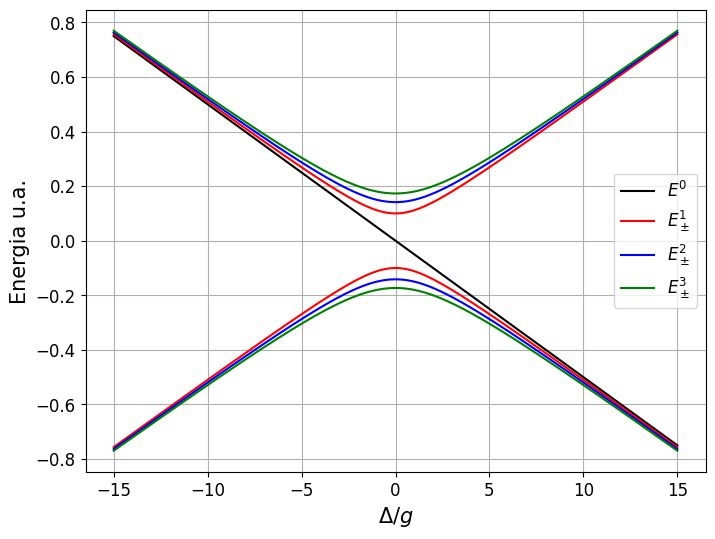
\includegraphics[width=0.7\textwidth]{figuras/ch3/relacion energia detunning jcm simple.png}
    \caption{Relaci\'on energ\'ia detunning para el modelo de Jaynes-Cummings. La diferencia de energ\'ia entre los estados de un mismo nivel para $\Delta=0$ es $2g\sqrt{n}$.}
    \label{fig:relación energia detunning jcm1}
\end{figure}
En la figura \ref{fig:relación energia detunning jcm1} se observan las curvas de energ\'ia en funci\'on del detunning para diferentes niveles. Lo primero que tenemos que observar es que en el caso resonante, es decir $\Delta=0$, los autoestados del sistema son los estados maximamente entrelazados de Bell
\begin{equation}
    \ket{\psi_\pm^n}=\frac{1}{\sqrt{2}}(\ket{gn}\pm\ket{e,n-1})
\end{equation} 
y la diferencia de energ\'ia entre los autoestados es $\Delta E^n =E^n_+-E^n_-=2g\sqrt{n}$. En el caso muy lejos de resonancia podemos asumir que $\Delta \gg g $, y entonces los autoestados coinciden en este l\'imite con los estados de la base, 
\begin{equation}
    \begin{aligned}
        \ket{\psi^n_+}=\ket{e,n-1} \\
        \ket{\psi^n_-}=\ket{g,n}
    \end{aligned}
\end{equation}
Ac\'a hay una sutileza, y es que si $\Delta>0$, entonces $\ket{e,n-1}$ es el estado de mayor energ\'ia y la notaci\'on coincide con la energ\'ia, pero si $\Delta<0$ entonces el estado $\ket{\psi^n_+}$ es el estado de menor energ\'ia. 
Un efecto interesante es que en el caso de alta desinton\'ia, podemos calcular la diferencia entre la energía del autoestado exacto del Hamiltoniano $\ket{\psi_\pm^n}$ y la energía asintotica a la que tiende, que es la energía de los estados de la base $\ket{g,n},\ket{e,n-1}$. Esta diferencia ... \textcolor{red}{VOLVER A ESTO Y VER SI DEJARLO O SACARLO. EVENTUALMENTE COMPLETAR.}
\begin{equation}
    \begin{aligned}
        \Delta E_{e,n-1}=E_+^n-E^{(0)}_{e,n-1}=\frac{g^2}{\Delta}n
        \Delta E_{g,n}=E_-^n-E^{(0)}_{g,n}=-\frac{g^2}{\Delta}n
    \end{aligned}
\end{equation}
El resultado importante de esta diferencia de energias es que aun en ausencia de fotones en la cavidad $n=0$, hay una diferencia entre las energias entre el Hamiltoniano del átomo, y del $H_{JC}$. Este efecto es el \textit{Lamb Shift} y nos dice que el vac\'io electromagnetico induce un corrimiento en la energ\'ia de los estados. Esto es importante notarlo, porque para el caso de dos átomos tambien est\'a manifiesto.

\subsection{Fase geométrica en el JCM}
Vamos a analizar la fase de Berry y la fase geométrica en la aproximación cinemática.
\subsubsection{Fase de Berry}
Para ver la fase de berry tenemos que tener un parámetro de control en el Hamiltoniano, el cual varía lentamente. Para esto necesitamos aplicar una transformación unitaria de corrimiento de fase al Hamiltoniano original \ref{eq3:hamiltoniano jcm} $R=\exp{-i\Omega a^\dagger a}$, que queda
\begin{equation}
    H=\frac{\Delta}{2}\sigma_z+g(a^\dagger \sigma_e^{-i\Omega}-+a\sigma_+e^{i\Omega})
\end{equation}
que ahora depende explicitamente del parámetro externo de control $\Omega$. Los autoestados de este nuevo Hamiltoniano se obtienen aplicando esta misma transformación sobre los autoestados del Hamiltoniano original. Si el parámetro de control varia lentamente entre 0 y $2\pi$, entonces estamos dentro de las hipotesis propuestas por Berry, y podemos calcular la fase de Berry mediante la ecuación \ref{eq2:fg berry}:
\begin{equation}
    \psi_a^n=i\oint_Cd\Omega\bra{\psi_\pm^n}R(\Omega)^\dagger \frac{d}{d\Omega}\ket{\psi_\pm^n}=\pi(1\pm \cos(\theta_n))
\end{equation}

que es no trivial incluso para $n=0$, lo que nos dice que incluso el vacio electromagnetico introduce una corrección en la fase de Berry.
\subsubsection{Aproximación Cinemática}
Para comparar ambos metodos, ahora vamos a calcular la fase geométrica utilizando la aproximación cinemática aunque este abordaje es más general de lo necesario en este caso.
Si se considera que el estado inicial es un atuoestado del Hamiltoniano, como los estados $\ket{\psi_\pm^n}$, entonces la fase geométrica en este caso se anula. Pero si se considera un estado inicial, por ejemplo $\ket{\psi(0)}=\ket{e,n}$, entonces el estado a tiempo $t$ resulta
\begin{equation}\label{eq3:fg berry jcm}
    \ket{\psi(t)}=(\cos^2\theta_ne^{-iE_+^nt}+\sin^2\theta_ne^{iE_+^nt})\ket{e,n}-i \sin\theta_n\sin(E_+^nt)\ket{g,n+1}
\end{equation}
La fase geometrica acumulada \ref{eq2:fg cinematica unitaria} es
\begin{equation}\label{eq3:fg unitaria jcm}
    \phi_u[C]=-\pi(1-\cos\theta_n)\frac{t}{T} +\arg\left\{ 1+e^{2\pi i \frac{t}{T}}\frac{\Omega_n-\Delta}{\Omega_n+\Delta} \right\}
\end{equation}
con $T=\frac{2\pi}{\Omega_n}$ es un período correspondiente a la frecuencia de Rabi $\Omega_n$. Esta expresión y la antrior \ref{eq3:fg berry jcm}, deberian coincidir cuando $t=T$, que se corresponde con un ciclo cerrado. En este caso ($t=T$) se obtiene
\begin{equation}
    \phi_u=-\pi(1-\cos\theta_n)
\end{equation}
La diferencia de signos se puede explicar comparando las curvas descritas por la esfera de Bloch para cada evolución. 
\begin{figure}[H]
    \centering
    \begin{subfigure}[h]{0.49\textwidth}
        \centering
        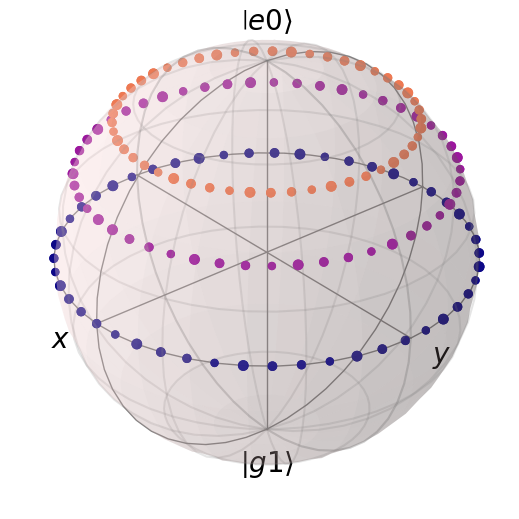
\includegraphics[width=\textwidth]{figuras/ch3/bloch berry.png}
        \caption{Evolución adiabática} 
        \label{fig3:bloch berry}
    \end{subfigure}
    \hfill
    \begin{subfigure}[h]{0.49\textwidth}
        \centering
        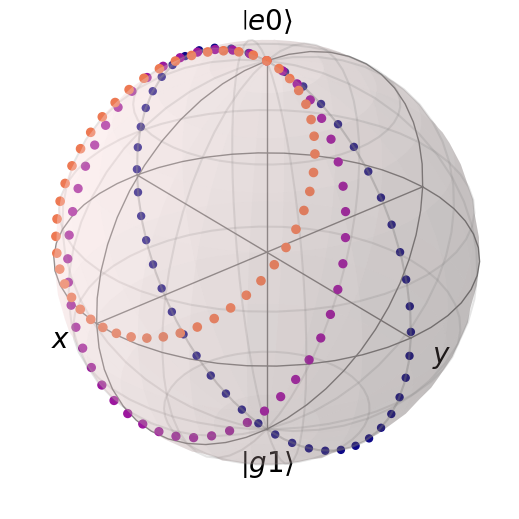
\includegraphics[width=\textwidth]{figuras/ch3/bloch cinematica.png}
        \caption{Enfoque cinemático}
        \label{fig3:bloch cinematica}
    \end{subfigure}
    \caption{}
    \label{fig3:esfera de bloch jcm}
\end{figure}
En el caso \ref{eq3:fg berry jcm}, correspondiente a la figura \ref{fig3:bloch berry}, los autoestados son los autoestados $R(\Omega)\ket{\psi_\pm^n}=e^{-i\Omega \hat n}\ket{\psi_\pm^n}$, entonces al variar $\Omega\in [0,2\pi]$ la trayectoria es simplemente un circulo en la esfera de Bloch. En cambio, en el segundo caso, si preparamos el sistema inicialmente en el estado $\ket{e,n}$ y lo dejamos evolucionar por la acción de H durante un tiempo, la trayectoria ahora no son circulos horizontales en la esfera, sino que parten del polo norte, que es el estado $\ket{e,n}$, y luego hace una trayectoria ovalada, para finalmente volver al punto inicial de partida a un tiempo $t=T$. La diferencia en el signo se explica a travez de la transformación que nos lleva de una curva a la otra. Para esto, necesitamos de una rotacion rigida, y una inversion de la parametrizacion, por su parte, esta ultima, introduce un signo negativo, cosa que se ve claramente en la ecuacion \ref{eq3:fg unitaria jcm} al cambiar $t\rightarrow -t$.

\textcolor{red}{aca puedo intentar de agregar el caso con medio kerr. Creo que no es tan complicado y el problema de autocosas ya lo tengo medio resuelto en papel desde hace un tiempo, pero lo tengo que revisar a ver si esta bien y lo tengo que completar, pero puede estar bueno para entender que le hace a la FG desde el vamos.}

\section{JCM disipativo}


Habiendo desarrollado el análisis de la fase geométrica acumulada por el sistema átomo-cavidad en la situación ideal de completo aislamiento, se aborda ahora el estudio para el escenario más realista en el que el mismo sistema se encuentra en interacción con un entorno. El problema se trata para la implementación específica en estructuras semiconductoras, en las que un punto cuántico (al cual se sigue, sin embargo, refiriendo como átomo o sistema de dos niveles) se ubica en una nano o micro-cavidad.

Siguiendo \cite{80}, en este capítulo se estudia en detalle la fase geométrica acumulada en un modelo de Jaynes-Cummings disipativo, como caso paradigmático dentro del campo de la electrodinámica en cavidades. Se considera que los principales mecanismos por los cuales el sistema “átomo + modo” interactúa con el entorno son el flujo de fotones a través de las paredes de la cavidad y el continuo e incoherente bombeo del sistema de dos niveles, lo que conforma un escenario frecuente en electrodinámica de cavidades semiconductoras \cite{81,82,83}. 

Para poder modelar estos mecanismos, se emplea la ecuación maestra fenomenológica de Lindblad
\begin{equation}\label{eq3:lindblad}
\dot{\rho}(t) = -i [H, \rho(t)] + \frac{1}{2} \sum_\alpha \big( 2L_\alpha \rho(t) L_\alpha^{\dagger} - \{ L_\alpha^{\dagger}L_\alpha, \rho(t) \} \big),
\end{equation}

, despreciando otros procesos con menor influencia en la dinámica como el desfasaje puro o el bombeo de fotones del entorno en la cavidad, considerando además que el entorno se halla a temperatura cero. Los operadores de Lindblad

\begin{equation}
L_\gamma = \sqrt{\gamma} \ a
\end{equation}
\begin{equation}
L_p = \sqrt{p} \ \sigma_+
\end{equation}

,representan la pérdida de fotones y el bombeo continuo e incoherente del átomo, respectivamente, con los parámetros $\gamma$ y $p$ denominados tasa de pérdida de fotones y amplitud del bombeo. 

El bombeo sobre el átomo es siempre secundario frente a la pérdida de fotones, lo cual nos da las relaciones $\frac{p}{g},\frac{p}{\gamma} \ll 1$, y la relación entre $\gamma$ y $g$ da lugar a dos regimenes que se diferencian con claridad \cite{50}-\cite{54}. El regimen de acoplamiento fuerte (SC o Strong Coupling) es cuando la interacción átomo-cavidad es mas fuerte que la disipación del entorno, es decir $\gamma /g <1$. En el caso contrario $\gamma/g>1$ estamos en el régimen de acoplamiento débil (WC o Weak Coupling). Para no generar confusiones, hay que destacar que en general, cuando en la literatura se habla de acoplamientos fuertes y debiles, se refiere a la interacción entre las partes del mismo sistema, pero en este caso, se esta haciendo referencia a la interacción del sistema con el entorno EN COMPARACIÓN con la interacción interna del sistema.

En esta ocación nos interesa resolver el problema restringiendonos al subespacio donde el átomo puede estar en cualquiera de sus dos estados, y nos restringimos al caso en donde la cavidad tiene 1 o 2 fotones, en consecuencia, se restringe el estudio a un subespacio truncado cuya base son los estados $\{ \ket{0}=\ket{g,0} ; \ket{1}=\ket{e,0} ; \ket{2}=\ket{-,1} \}$. Desarrollando explicitamente el sistema de ecuaciones dadas por la ecuación de Lindblad \ref{eq3:lindblad}, obtenemos que los elementos $\rho_{0i}$ quedan desacoplados de los demas:

\begin{equation}
    \begin{aligned}
        \dot \rho_{01} & =-\frac{p}{2} \rho_{01}+i\Delta\rho_{01}+ig\rho_{02} \\
        \dot \rho_{02} & =-\frac{p}{2} \rho_{02}-\gamma \rho_{02}+ig\rho_{01}
    \end{aligned}
\end{equation}
,con lo cual, si inicialmente los elementos de matriz $\rho_{0i}(0)=0$, permanecerán así durante toda la evolución del sistema. Para hacer una analogía y realizar una comparación con el caso unitario, se estudia la condición inicial $\rho(0)=\ketbra{e,0}{e,0}$, que satisface esta condición, de manera que se espera que el estado $\rho(t)$ exciba una estructura diagonal por bloques. El primer bloque de 1x1 representando al estado $\ket{0}$, y luego un bloque de 2x2 que describe la dinámica entre los estados $\ket{1}$ y $\ket{2}$. Las ecuaciones son
\begin{equation}
\begin{aligned}
\dot{\rho}_{00} &= -p \rho_{00} + \gamma \rho_{22}, \\
\dot{\rho}_{11} &= -i g (\rho_{21} - \rho_{12}) + p \rho_{00}, \\
\dot{\rho}_{22} &= -i g (\rho_{12} - \rho_{21}) - \gamma \rho_{22}, \\
\dot{\rho}_{12} &= -i g (\rho_{22} - \rho_{11}) - i \Delta \rho_{12} - \frac{\gamma}{2} \rho_{12}.
\end{aligned}
\end{equation}

que se resuelven numericamente para acceder al estado $\rho(t)$ a tiempo $t>0$. 

\textbf{[Placeholder para Figura: Evolución dinámica de elementos de matriz]}

El análisis de esta sección permite establecer la relación entre los efectos de disipación y la acumulación de la fase geométrica, así como determinar las condiciones bajo las cuales el sistema mantiene coherencia cuántica suficiente para aplicaciones experimentales.

	\chapter{Jaynes-Cummings de dos átomos, no lineal, medio Kerr}
\label{ch4_dinamica}

%CAMBIAR ESTO PARA PERSONALIZARLO A MI GUSTO
\pagestyle{fancy}
\fancyhf{}
\fancyhead[LE]{\nouppercase{\rightmark\hfill}}
\fancyhead[RO]{\nouppercase{\leftmark\hfill}}
\fancyfoot[LE,RO]{\hfill\thepage\hfill}

En este capitulo se extiende el modelo de Jaynes-Cummings presentado en el capitulo \ref{ch3_jcm}, agregandole nuevas cosas. Lo mas importante es que ahora vamos a tener dos átomos dentro de una misma cavidad. En la literatura en general, el JCM fue extendido para considerar dos cavidades donde cada una tiene su propio átomo, y usando una condición inicial entrelazada se puede hacer interactuar ambas cavidades REFS. El camino que se tomó en este trabajo, es un tanto fuera de lo convensional ya que no hay muchos estudios sobre este sistema. El principal obstaculo que presenta este problema, es que el espacio de Hilbert crece mucho y se torna inmanejable analiticamente; como bien ya sabemos, el JCM tiene subespacios de 2 dimensiones que no se mezclan, y utilizando esta estrategia vamos a ver que en este caso tenemos subespacios de 4x4 que tampoco se mezclan en el caso unitario. Esto nos permite encontrar algunas expresiones analiticas, pero en general se utilizaran métodos númericos para analizar la dinamica. \newline
Este capitulo entonces seguira un hilo conductor, partiendo desde el caso mas sencillo hasta llegar a analizar cuales son los efectos de los diferentes parámetros en el problema. 
	Primero vamos a considerar una cavidad perfecta, es decir sin disipaci\'on, agregandole el segundo átomo, vamos a intentar de entender cual es el efecto de este sobre el modelo de un solo átomo. Para esto haremos un analisis poblacional, y de observables como la entropia reducida, la concurrencia, las matrices de pauli. Una vez agregado el segundo átomo, vamos a prender las interacciones de a una y vamos a analizar cuales son sus efectos. Luego, vamos a comparar esto con el caso en donde la cavidad presenta perdidas. Principalmente, nos centraremos en un analisis del entrelazamiento, ya que esta es la cualidad mas interesante que tenemos en el ambito de la informaci\'on cu\'antica. 

\textcolor{blue}{Luego, se analizar\'a el problema para dos átomos, primero en el caso que estos no interact\'uan
directamente entre si, sino que lo hace indirectamente a travez de la cavidad. La comparativa entre
esta situación y la mas comun, donde los átomos interactuan mediante sus espines o sus momentos
dipolares, es muy rica porque nos permite discernir con claridad cual es el efecto de la cavidad
y cual de la interacción entre los átomos a la hora de entrelazarse e intercambiar energía.
El problema de dos átomos tiene una peculiaridad al elegir las condiciones iniciales, ya que la
dinamica depende de esta eleccion, y hay muchas diferentes configuraciones interesantes, por un lado
por la gran dimension del espacio, y por otro lado, esta la posibilidad de jugar con las simetrias.
Surge asi la pregunta de si es importante, o si tiene sentido, teniendo dos átomos indistinguibles
en una cavidad, que la condición inicial sea asimetrica ante intercambio. 
}

\section{Modelo de dos átomos y solucion unitaria}
En este trabajo, nos vamos a concentrar en una extension del modelo, donde vamos a ubicar dos átomos dentro de la cavidad. Estos átomos pueden interactuar entre si, y con la cavidad, y ademas agregaremos no-linealidades en el acoplamiento y en el medio.
Vamos a usar un modelo de Jaynes-Cummings para describir la interacci\'on entre el campo electromagn\'etico y los átomos. Adem\'as supondremos que el acoplamiento depende de la cantidad de fotones y los átomos podr\'an interactuar entre si mediante un termino tipo Ising y otro tipo dipolo-dipolo. Recordemos que para estamos asumiendo que vale la aproximaci\'on de onda rotante ($\omega_0 \sim \omega$) y $g << \omega,\omega_0$.
Entonces, el Hamiltoniano que describe este problema es el siguiente:

\begin{equation}
\begin{split}
     \hat H & =\underbrace{\hbar \omega_0 h(\hat n) \hat n }_{\hat H_F}+\underbrace{\frac{\hbar \omega}{2}(\hat\sigma_Z^{(1)}+\hat\sigma_Z^{(2)})}_{\hat H_A}   \\ 
     & + \underbrace{\hbar g(\hat\sigma_+^{(1)}\hat a f(\hat n)+\hat\sigma_-^{(1)}f(\hat n) \hat a^\dagger + \hat\sigma_+^{(2)}\hat a f(\hat n)+\hat\sigma_-^{(2)}f(\hat n) \hat a^\dagger)}_{H_{FA}} + \\ & \underbrace{2\hbar \kappa (\hat \sigma_-^{(1)}\hat \sigma_+^{(2)}+\hat \sigma_+^{(1)}\hat \sigma_-^{(2)}) + \hbar J \hat \sigma_Z^{(1)}\hat \sigma_Z^{(2)}}_{H_{AA}}
\end{split}
\end{equation}

donde $\hat a$ es el operador de aniquilaci\'on del fot\'on, $\omega_0$ y $\omega$ son las frecuencias del fot\'on y del átomo respectivamente, $g$ es la constante de acoplamiento, las constantes $J$ y $\kappa$ son los par\'ametros de Ising y de dipolo-dipolo para las interacciones átomo-átomo, y los operadores $\sigma^{(i)}$ son las matrices de Pauli que act\'uan sobre el átomo i-esimo. Finalmente, las funciones $h(\hat n)$ y $f(\hat n)$ son las que van a dar cuenta de la no linealidad dependiente del numero de fotones de la cavidad $\hat n = \hat a^\dagger \hat a$. 

Tomando un medio tipo Kerr la funci\'on $h(\hat n)=1+\frac{\chi}{\omega_0}\hat n$ \cite{}\textcolor{red}{(CITA)}, y la funci\'on $f(\hat n) =1$ si tomamos un acoplamiento lineal, y $f(\hat n) = \sqrt{\hat n}$ si consideramos un acoplamiento tipo Buck-Sukumar \cite{}\textcolor{red}{(CITA)}

En este punto es normal hacer una transformaci\'on unitaria  $K = \exp\left\{-i \omega t (\hat a^\dagger a + \sigma_z/2)\right\}$ para dejar el Hamiltoniano en funci\'on del Detuning $\Delta (\sim 0)$. 

\begin{equation}
\begin{split}
     \hat H_I & =\hbar \chi \hat n^2+\frac{\hbar \Delta}{2}(\hat\sigma_Z^{(1)}+\hat\sigma_Z^{(2)})   \\ 
     & + \hbar g(\hat\sigma_+^{(1)}\hat a f(\hat n)+\hat\sigma_-^{(1)}f(\hat n) \hat a^\dagger + \hat\sigma_+^{(2)}\hat a f(\hat n)+\hat\sigma_-^{(2)}f(\hat n) \hat a^\dagger) \\ 
 & + 2\hbar \kappa (\hat \sigma_-^{(1)}\hat \sigma_+^{(2)}+\hat \sigma_+^{(1)}\hat \sigma_-^{(2)}) + \hbar J \hat \sigma_Z^{(1)}\hat \sigma_Z^{(2)}
\end{split}
\end{equation}\label{eq4:H}
Este es el Hamiltoniano con el que vamos a trabajar, así que a partir de ahora vamos a olvidarnos del subíndice I. Obsérvese que el caso de $\chi=0$ es el caso de un medio lineal. 
\textcolor{blue}{ACA PUEDO AGREGAR UN ESQUEMA DE COMO SERIA.} En este esquema se ve como seria el experimento planteado. 

Este Hamiltoniano se puede resolver analíticamente para el caso de una cavidad sin perdidas. En analogía con el caso de 1 átomo, vamos a elegir la base de N excitaciones, donde esperamos que estos subespacios queden invariantes, es decir, que el Hamiltoniano sea diagonal por bloques, pero como ahora tenemos 2 átomos, tenemos que elegir una base que respete simetrías, para N excitaciones los estados de la base son $\left\{\ket{ggn},\frac{1}{\sqrt{2}}(\ket{eg,n-1}+\ket{ge,n-1}),\ket{ee,n-2},,\frac{1}{\sqrt{2}}(\ket{eg,n-1}-\ket{ge,n-1})\right\}$. En esta base, el Hamiltoniano se diagonaliza por bloques y el bloque de N excitaciones queda
El problema unitario se puede resolver analíticamente. Esto esta hecho en el paper de los autores \textit{O de los Santos-Sánchez
, C González-Gutiérrez and J Récamier}, titulado \textit{Nonlinear Jaynes–Cummings model for two
interacting two-level atoms} \cite{paper:santos}\textcolor{red}{(CITA)}. 
\textcolor{red}{Ac\'a tengo que pasar las cuentas a latex, pero las hice en papel para ver si entend\'ia todo.}
Para resolver el problema lo primero que hacemos es notar que el Hamiltoniano conserva el numero de excitaciones, es decir $[H,\hat N]=0$, y en esta situación es sabido que el Hamiltoniano de JC es diagonal por bloques si elegimos convenientemente la base, esta es la que agrupa los estados con misma cantidad de excitaciones $\hat N = \hat n + \hat \sigma_+^{(1)}\hat \sigma_-^{(1)}+\hat \sigma_+^{(2)}\hat \sigma_-^{(2)}$: 
\begin{equation}
\begin{split}
    & \left\{\ket{\Phi^{(n)}_1}=\ket{ggn},\ket{\Phi^{(n)}_2}=\frac{1}{\sqrt{2}}(\ket{egn-1}+\ket{gen-1}),\ket{\Phi^{(n)}_3}=\ket{een-2},\right. \\
& \left. \ket{\Phi^{(n)}_4}=\frac{1}{\sqrt{2}}(\ket{egn-1}-\ket{gen-1})\right\} 
\end{split}
\label{ec4:base}
\end{equation}
,donde se eligi\'o esta combinaci\'on particular porque el ultimo estado de la base, que es impar ante intercambio, queda desacoplado de los otros, simplificando el problema. Esto se ve al evaluar los elementos de matriz del Hamiltoniano $H_{i,j}=\bra{\Phi_i}\hat H \ket{\Phi_j}$, este queda en bloques, y el subespacio correspondiente a $n$ excitaciones $\hat H^{(n)}$ es una matriz de 4x4
\begin{equation}
    \frac{\hat H^{(n)}}{\hbar}=
    \begin{pmatrix}
     \chi n^2 - \Delta +  J & \sqrt{2} g f(n)\sqrt{n} & 0 & 0 \\
    \sqrt{2} g f(n)\sqrt{n} &  \chi (n-1)^2  -  J + 2 k & \sqrt{2} g f(n-1)\sqrt{n-1} & 0 \\
    0 & \sqrt{2} g f(n-1)\sqrt{n-1} &  \chi (n-2)^2 +  \Delta +  J & 0 \\
    0&0&0& \begin{aligned} 
                 & \chi (n-1)^2  \\ 
                 &-  J - 2 k
        \end{aligned}
    \end{pmatrix}
\end{equation}
Vemos claramente que el estados impar ante intercambio esta aislado, y entonces es autoestado del problema, y por lo tanto evoluciona solo y no se mezcla con los otros estados. Esto nos sirve porque ahora, para terminar de resolver el problema, tenemos que diagonalizar la matriz de 3x3. Cabe aclarar que esta matriz solo es valida para $n\geq 2$, ya que los subespacios con $N=0,1$ no tienen 4 estados. En estos casos la soluci\'on del problema de autovalores es mas sencilla aun, as\'i que solo dejaremos los resultados. A partir de ahora se usar\'a como convención $\hbar=1$. \newline
Para resolver el problema de autovalores de la matriz de 3x3 utilizamos la fórmula de Cardano para conseguir las ra\'ices triples que nos aparecen en el polinomio caracter\'istico, y entonces encontramos que los autovalores son
\begin{equation}
    E_j^{(n)}=-\frac{1}{3}\beta_n+2\sqrt{-Q_n}\cos{\left(\frac{\theta_n+2(j-1)\pi}{3}\right)}
    \label{ec4:autoenergias}
\end{equation}
para $j=1,2,3$, y donde 
\begin{equation}
    \theta_n=\cos^{-1}\left(\frac{R_n}{\sqrt{-Q_n^3}}\right)
\end{equation}
\begin{equation}
    \begin{aligned}
        Q_n & = \frac{3\gamma_n-\beta_n^2}{9} \\
        R_n & = \frac{9\beta_n\gamma_n-27\eta_n-2\beta_n^3}{54} \\
        \beta_n & = - \left( \chi(n^2+(n-1)^2+(n-2)^2)+J+2k\right) \\
        \gamma_n & = (\chi(n-1)^2 - J + 2k)(x(n-2)^2+\chi n^2+2J) \\ 
        & +(\chi (n-2)^2+\Delta+J)(x n^2-\Delta+J)-2g^2(n^{2a}+(n-1)^{2a}) \\ 
        \eta_n &= -(\chi n^2-\Delta+J)(\chi(n-2)^2+\Delta+J)(\chi(n-1)^2-J+2k) \\
        &+2g^2 \left[  \chi(n-2)^2n^{2a}+\chi n^2(n-1)^{2a}+\Delta\left(n^{2a}-(n-1)^{2a}\right) +J(n^{2a}-(n-1)^{2a})\right]
    \end{aligned} 
    \label{ec4:parametros solucion}
\end{equation}
donde $a=\frac{1}{2}$ se corresponde con acoplamiento lineal, es decir, $f(n)=1$, y $a=1$ a Buck-Sukumar $f(n)=\sqrt{n}$. Los autovalores ser\'an reales si $Q_n^3+R_n^2<0$.
Con esto podemos escribir los autovectores:
\begin{equation}
    \begin{split}
        \ket{u_j^{(n)}} &= \frac{1}{N_j^{(n)}} \bigg[ \left((E_j^{(n)} - H_{22}^{(n)})(E_j^{(n)}-H_{33}^{(n)}) - H_{23}^{(n)^2} \right) \ket{\Phi_1^{(n)}} \\ &+ H_{21}^{(n)}(E_j^{(n)}-H_{33}^{(n)})\ket{\Phi_2^{(n)}} + H_{23}^{(n)}H_{12}^{(n)}\ket{\Phi_3^{(n)}}\bigg]
    \end{split}
\end{equation}
Obviamente no nos olvidemos del estado $\ket{\Phi_4^{(n)}}$, que tambi\'en es autoestado, con autovalor $E_4^{(n)}=\chi(n-1)^2-J-2k$.
Para el subespacio de $N=0$ solo tenemos un vector $\ket{\Phi_1^{(0)}}=\ket{gg0}$ y su autovalor es $E_1^{(0)}=-\Delta+J$.
Para $N=1$ tenemos 3 vectores en el subespacio, y las autoenergías son
\begin{align}
    E_{1,2}^{(1)} &=\frac{\chi -\Delta}{2} +k \pm \sqrt{2g^2+(k-J+\frac{\Delta -\chi}{2} )^2} \\
    E_3^{(1)} & = -2k-J 
\end{align}
y sus autovectores
\begin{align}
    \ket{u_{1,2}^{(1)}}&=\frac{1}{N_{1,2}^{(1)}}(-\sqrt{2}g\ket{gg1}+ \left(\frac{\chi-\Delta}{2}+J-k \mp \sqrt{2g^2+(k-J+\frac{\Delta -\chi}{2} )^2} \right)\dfrac{\ket{eg0}+\ket{ge0}}{\sqrt{2}}\\
    \ket{u_3^{(1)}}&= \frac{1}{\sqrt{2}}(\ket{eg0}-\ket{ge0})
\end{align}
Con esto, podemos resolver analíticamente la evolución temporal de cualquier estado inicial.
Para esto solo tenemos que desarrollar el estado inicial en términos de los autovectores, y la evolución temporal esta dada por
\begin{equation}
\ket{\psi(t)}=e^{-iHt}\ket{\psi(0)}=\sum_{j,n} c_j^{(n)}e^{-iE_j^{(n)}t}\ket{u_j^{(n)}}
\end{equation}
donde $c_j^{(n)}=\braket{u_j^{(n)}}{\psi(0)}$.
La complejidad de estas expresiones hace complicado conseguir conclusiones interesantes,aun asi, algo que se puede notar, es la diferencia fundamental que se encuentra para las energías con un numero total de excitaciones $N=1$ y $N>1$. Si se observa el factor que esta antes de la raiz cuadrada,  se ve que para el caso en que $N \geq 2$ tenemos un $\frac{1}{3}\beta_n$ que solo depende de $\chi$, $J$, $k$ y $n$. Mientras tanto, en el caso de $N=1$, este factor depende del detunning $\Delta$. Esto es interesante, ya que uno podría pensar que la formula para $N$ excitaciones se puede generalizar para incluir $N=0,1$, pero la fundamental diferencia de tener mas o menos estados que interactúan entre si, da lugar a efectos fundamentalmente diferentes. Si uno mira en detalle las cuentas, se percata de que en el caso de $N=1$ este factor $\Delta$ aparece, ya que en la matriz Hamiltoniana el único estado con $N=1$ que tiene un termino que incluye al detunning, es el estado $\ket{gg1}$, y los otros dos estados al ser un átomo excitado y otro no, el termino de detunning se cancela. Por lo tanto, este termino con $\Delta$ sobrevive, al contrario que en todos los demás subespacios, ya que tenemos por un lado el termino del $\ket{ggn}$ que nos aporta un $\Delta$, y el termino de $\ket{ee,n-2}$ que nos aporta otro $\Delta$ pero con el signo cambiado, y elimina la contribución del primer estado a la energía. Esto es muy interesante, ya que para $N=1$, si aumentamos el detunning, no solo se separan los niveles de energía, sino que también hay una asimetría por el termino independiente. Para analizar esto en detalle, en la figura \ref{fig:relación energia detunning} se observan las energías de los diferentes niveles en función del detunning. 

\begin{figure}
    \centering
    \begin{subfigure}[h]{0.49\textwidth}
        \centering
        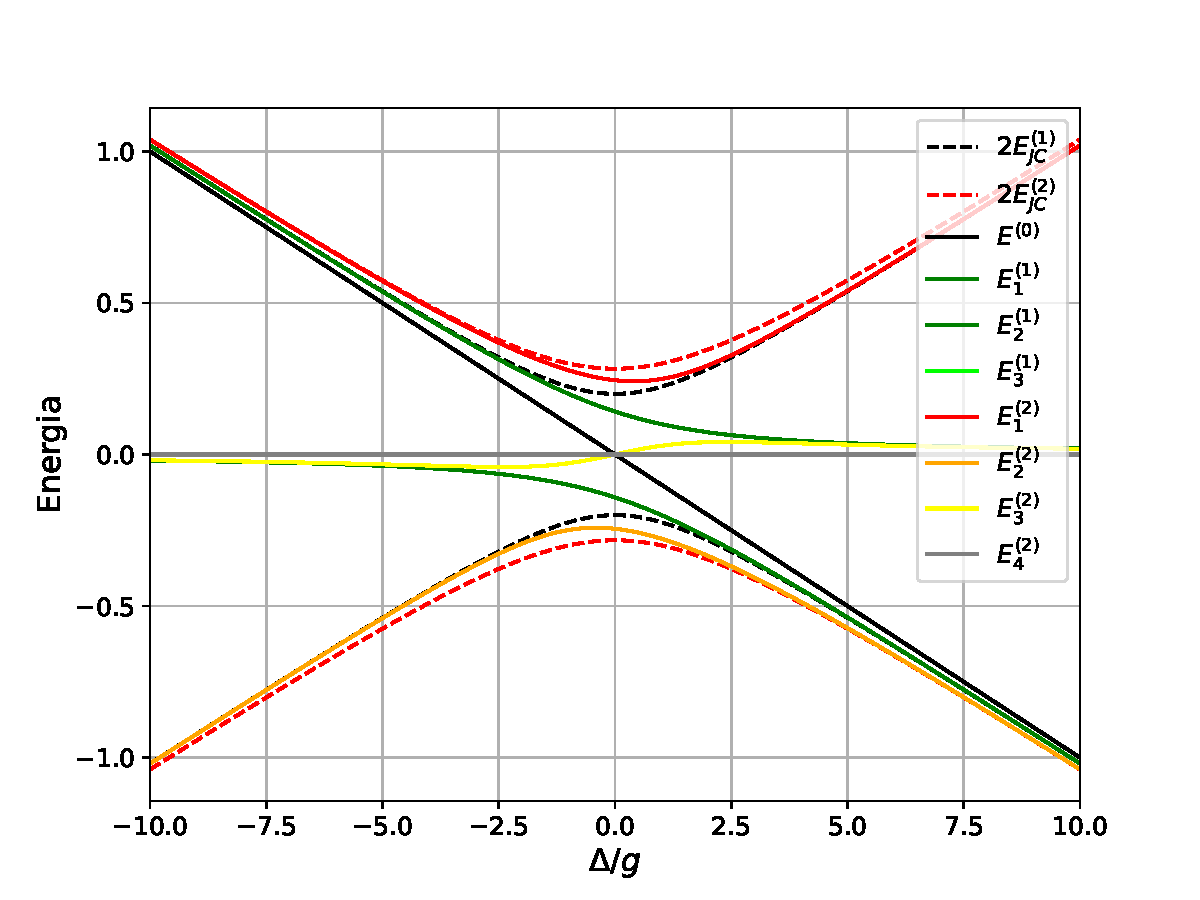
\includegraphics[width=\textwidth]{figuras/ch4/relacion_energia_detunning1.pdf}
        \caption{$k=J=0$}
        \label{fig:relación energia detunning 1}
    \end{subfigure}
    \hfill
    \begin{subfigure}[h]{0.49\textwidth}
        \centering
        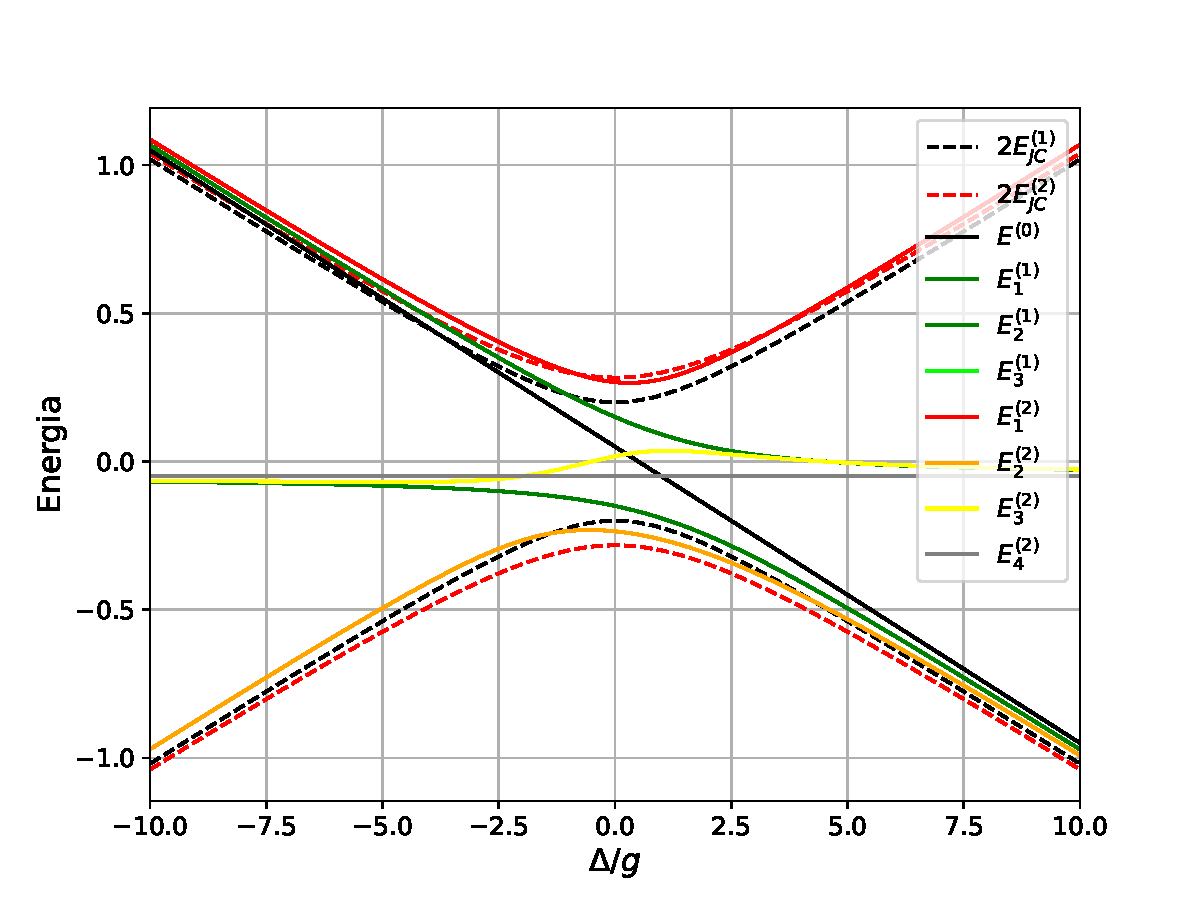
\includegraphics[width=\textwidth]{figuras/ch4/relacion_energia_detunning2.pdf}
        \caption{$J\neq 0$}
        \label{fig:relación energia detunning 2}
    \end{subfigure}
       \caption{Relación entre energía y detunning para los diferentes niveles de energía del problema. Las lineas solidas muestran la energía de los estados del JC doble con N=0 (negro, solido), N=1 (verde oscuro y lima, solido) y N=2 (rojo, naranja, amarillo y gris; solido). Cambien se muestran los niveles de energía del JC de un átomo para N=1 (negro; rayado) y N=2 (rojo; rayado). Obsérvese que las energías del JC de un átomo están multiplicadas por 2.}
       \label{fig:relación energia detunning}
\end{figure}
En esta figura \ref{fig:relación energia detunning 1} se observan las energías de los primeros niveles para el modelo de un átomo, mostrados con lineas rayadas, y de dos átomos, con lineas solidas; para esta figura se tomaron átomos que no interactúan ($k=J=0$) y una cavidad lineal ($\chi=0$). Se puede ver que, si bien el modelo de dos átomos tiene estructuras mas complicadas, son similares a las de 1 átomo. En primer lugar, los estados con N=2 (rojo y naranja; solido) tienen una forma igual a la de JC de 1 átomo, si bien esta un poco desfasada, es interesante ver como las lineas tienen una coincidencia muy grande, recordando que en el gráfico las lineas rayadas están multiplicadas por 2, esto nos da una interpretación bastante buena, y es que la energía de dos átomos no interactuantes en una cavidad es igual (o muy parecida) a dos veces la energía de 1 átomo en una cavidad. \textcolor{red}{Esto tengo que chequear con cuentas} \textcolor{blue}{Creo que esto se debe al corrimiento Lamb, ya que ahora tenemos dos átomos que interactúan con el vacío, entonces el corrimiento es 1 unidad mas grande en los extremos, que es justamente lo que vemos en el gráfico, cuando el detunning es muy negativo, la energ\'ia tiende a ser igual a la de un JC simple con 2 excitaciones, y cuando el detunning es muy positivo, entonces tiende a la de 1 excitaci\'on; esta asimetr\'ia para $\Delta>0$ y $\Delta<0$ se observar\'a en resultados posteriores.} Por otro lado, se puede observar lo que se había comentado anteriormente, que la energ\'ia de los estados con $N=1$ tienen un t\'ermino fuera de la raíz, que hace que sea mas asim\'etrico a\'un. Normalmente, en el JC de 1 átomo, ya que todos los niveles de energía tienen una forma funcional igual, este termino de afuera de la raíz se le puede agregar o quitar como un offset en la energía del estado fundamental, la diferencia con este caso es que, no todos los niveles de energía presentan esto, entonces si agregamos un offset, igualmente habría una diferencia. 

Otra cosa interesante de notar es que si la cavidad es lineal, entonces los estados antisimetricos de diferentes excitaciones $\frac{1}{\sqrt{2}}(\ket{eg,n}-\ket{ge,n})$ y $\frac{1}{\sqrt{2}}(\ket{eg,n'}-\ket{ge,n'})$, estan degenerados en energía.

Una vez estudiados los niveles de energía y comparados con el caso de 1 átomo, vamos a proseguir con la dinámica del problema, que en el caso unitario puede resolverse analíticamente, pero a\'un así, nos concentraremos en simulaciones numéricas.
Para comenzar, vamos a intentar de recuperar el caso de un átomo, asimetrizando el acoplamiento uno de los dos átomos que tenemos en la cavidad, y haciendo tender este a cero, es decir, vamos a trabajar con $k=J=0$ y vamos a agregar un parámetro adimensional $\alpha$ que solamente actúa sobre el átomo 2, y sirve de apantallamiento. Este parámetro $\alpha$ acompañara a las constantes de acoplamiento, por ejemplo el acoplamiento entre el átomo y la cavidad $g\rightarrow g\alpha$, tal que si $\alpha \rightarrow 0$ entonces el átomo quedara desacoplado de la cavidad. 

\section{Dinámica con apantallamiento}

Lo primero que se tiene que hacer es recuperar los resultados anteriores. Para aclarar, en la figura \ref{fig4:diagrama esquematico} se muestra un esquema de como es el problema que se esta trabajando, con los nombres que se le darán a las partes del sistema. Llamaremos átomo B al que esta apantallado mediante el parámetro adimensional $\alpha$, el indice A se referirá al otro átomo, y C a la cavidad. Entonces, para recuperar los resultados anteriores, se propone que $\alpha=0$ y la interacción entre los átomos $k=J=0$. De esta manera, se elige en analogía con el caso de 1 átomo, como estado inicial cualquier estado donde el átomo A sea excitado, y la cavidad C no tenga ningún fotón; por lo tanto se elige el estado inicial mas sencillo posible que cumple estas condiciones $\ket{\psi_0}=\ket{eg0}$. Si bien este apantallamiento no tiene un significado físico, y experimentalmente es imposible lograr estas condiciones, realizar este estudio sirve para entender cualitativamente los efectos de cada parámetro del problema, y también entender que el entrelazamiento entre los dos átomos, lleva a efectos impredecibles. La complejización del problema de 1 átomo al de 2 átomos es muy grande, y por eso es necesario ir de a poco.
\begin{figure}[H]
    \begin{minipage}[c]{0.67\textwidth}
        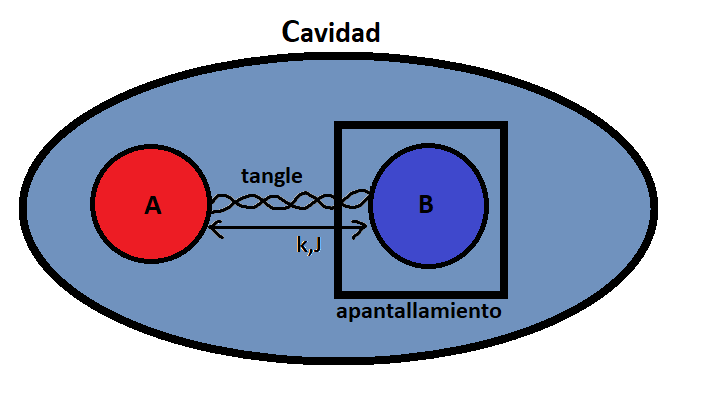
\includegraphics[width=\textwidth]{figuras/ch4/diagrama esquematico.png}
    \end{minipage}\hfill
    \begin{minipage}[c]{0.3\textwidth}
    \caption{Esquema del problema de estudio. Se nombran a las partes para referenciarlas fácilmente. Los átomos los llamamos A y B, donde el átomo B es el que sufre el apantallamiento que utilizaremos para recuperar los resultados anteriores. La cavidad la llamaremos C, esta puede contener una cantidad arbitraria de excitaciones, pero nos concentraremos principalmente en 0,1 y 2 excitaciones. Ambos átomos son de dos niveles, y en principio son idénticos e indistinguibles, pero se le agrega un apantallamiento artificial.
         } \label{fig4:diagrama esquematico}
  \end{minipage}
\end{figure}
Utilizando esta condición inicial se realiza una simulación numérica y se observan las poblaciones, y se espera recuperar la misma dinámica que en el caso de 1 átomo, ya que el átomo B no interactúa con ninguna de las otras partes del sistema A y C. Para poder representar el estado del sistema sobre una esfera de Bloch, se realiza una traza parcial sobre el átomo B, y así se obtiene la figura \ref{fig4:bloch delta}, donde se muestran 3 trayectorias correspondientes a diferentes valores del detunning, la linea azul es el caso resonante $\Delta=0$, y las trayectorias morada y naranja se corresponde con $\Delta=0.5g$ y $\Delta=2g$ respectivamente.
\begin{figure}[H]
    \begin{minipage}[c]{0.67\textwidth}
        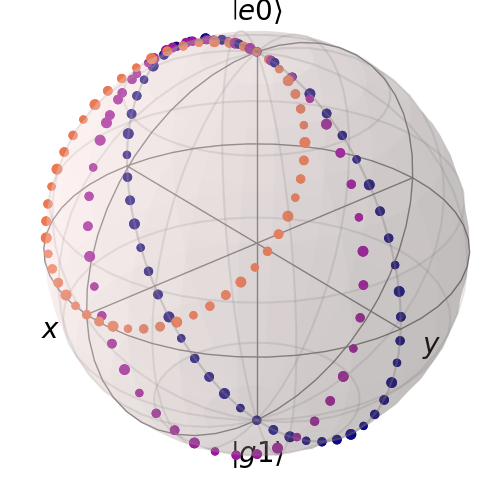
\includegraphics[width=\textwidth]{figuras/ch4/bloch eg0 bloch AC a=0 d=2.0 x=0.0 k=0.0 J=0.0 gamma=0.0 p=0.0.png}
    \end{minipage}\hfill
    \begin{minipage}[c]{0.3\textwidth}
    \caption{
         } \label{fig4:bloch delta}
  \end{minipage}
\end{figure}
Se observa como la dinámica entre estos dos estados es exactamente igual que la observada en la figura \ref{fig3:bloch cinematica}, ademas, como todos los puntos están sobre la superficie de la esfera, los estados son puros, diciéndonos que el estado global es separable, y entonces haber trazado sobre el átomo B no tuvo efecto sobre la dinámica entre el átomo A y la cavidad. Para corroborar esto se realiza un análisis poblacional mas general. \textcolor{red}{hacer gráfico con las probabilidades y ver que la probabilidad de eg0 + gg1 =1}
Lo siguiente que podemos analizar, que no se tenia la posibilidad cuando se tiene 1 átomo, es que se puede considerar una condición inicial entrelazada. Si bien los átomos no interactúan, y el átomo B esta aislado del universo, se puede entrelazar los átomos y luego se apagan las interacciones del átomo B. Por ejemplo, si se considera el estado inicial entrelazado $\ket{\psi_0}=(\ket{eg0}+\ket{ge0})/\sqrt{2}$, se obtiene 
\begin{figure}[H]
    \begin{minipage}[c]{0.67\textwidth}
        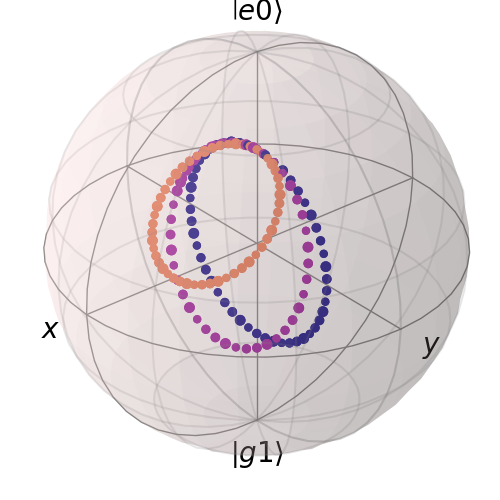
\includegraphics[width=\textwidth]{figuras/ch4/bloch eg0+ge0 bloch AC a=0 d=2.0 x=0.0 k=0.0 J=0.0 gamma=0.0 p=0.0.png}
    \end{minipage}\hfill
    \begin{minipage}[c]{0.3\textwidth}
    \caption{
         } \label{fig4:bloch delta}
  \end{minipage}
\end{figure}
Ahora, los estados no están sobre la superficie, lo que se interpreta como que estamos en presencia de un estado mixto. Al trazar sobre el átomo B, efectivamente se considera como si este fuese parte de un entorno. Al olvidarse de la dinámica del segundo átomo, se puede interpretar como que este se lleva un 50\% de probabilidad de llevarse la excitación, ya que no sabemos si inicialmente el átomo A o el átomo B es el que tiene la excitación. Entonces efectivamente tenemos un 50\% de probabilidad de que el estado de la cavidad sea $\ket{g0}$, y no evoluciona, y un 50\% de probabilidad de que la excitación este dentro de la cavidad, y por lo tanto vemos que la dinámica es la misma que en el caso anterior, pero con amplitudes menores. \textcolor{blue}{ACA IBA A DECIR ALGO, PERO ME PARECE QUE NO PUEDO PORQUE EL ESTADO ENTRELAZADO QUIZAS TIENE ALGUNAS COSAS RARAS. Uno puede adelantarse un poco, y deducir como se comporta la fase geométrica en estos dos casos. Por un lado, en el caso que el estado inicial no este entrelazado, la dinámica es exactamente igual que en el caso de 1 átomo, entonces la fase geométrica es la misma que \ref{eq3:fg unitaria jcm}, en cambio, cuando el estado inicial es el entrelazado, como la dinámica es igual que antes pero con un medio de la probabilidad, y luego el átomo B no evoluciona, entonces es autoestado y no acumula fase geométrica. Por lo tanto se puede concluir que en el caso entrelazado la FG va a ser la mitad que en el caso no entrelazado.}

Para analizar mas en detalle la dinámica, y para poder realizar comparaciones cuando se complejice el problema, se puede realizar un estudio poblacional, y también podemos mirar las entropías relativas y otros observables importantes.
En primer lugar, el caso separable $\psi_0=\ket{eg0}$, es idéntico al caso de 1 átomo, ya que el átomo B no evoluciona por estar totalmente aislado del sistema. Lo único que se puede resaltar es que, si se traza sobre la cavidad, que es algo que es útil para observar el entrelazamiento entre los átomos, lo único destacable es que el estado es mixto, ya que la evolución temporal del sistema átomo A-átomo B consta del átomo B en el estado fundamental $\ket{g}$, y el átomo A oscila entre el estado excitado y fundamental. La amplitud de oscilación y el grado de mixing entre los estados depende del detunning, siendo el caso $\Delta=0$ el de oscilaciones coherentes entre estados, y al aumentar $\Delta$ se este comportamiento.
En segundo lugar, cuando el estado inicial de los átomos no es separable por estar entrelazados $\ket{\psi_0}=(\ket{eg0} + \ket{ge0})/\sqrt{2}$, entonces la dinámica es un poco diferente. La figura \ref{fig4:fig4:dinamica eg0 sim resonante} muestra el caso de $\Delta=0$, donde se observan las evoluciones de las diferentes partes del sistema.

\begin{figure}[h]
    \centering
    \begin{subfigure}{0.49\textwidth}
        \centering
        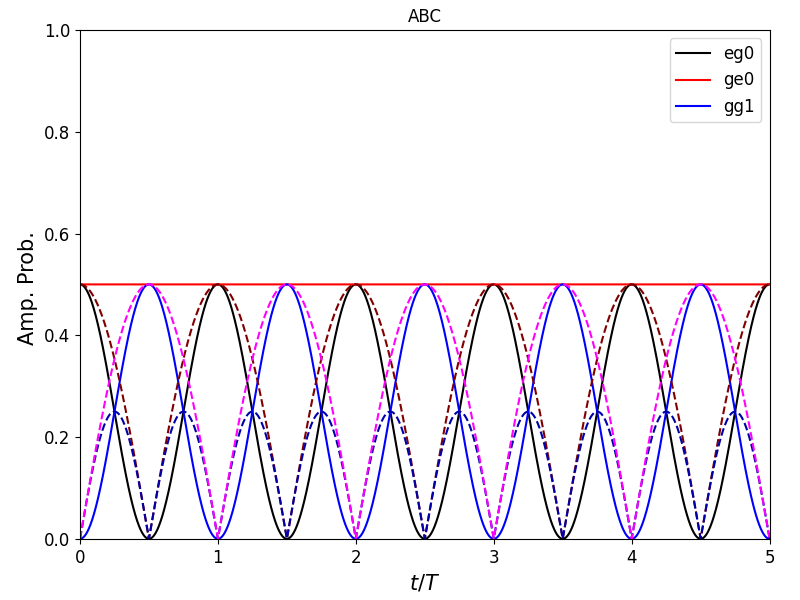
\includegraphics[width=\textwidth]{figuras/ch4/d eg0+ din ABC d=0.png}
        \caption{}
        \label{fig4:dinamica pob eg0 sim resonante}
    \end{subfigure}
    \hfill
    \begin{subfigure}{0.49\textwidth}
        \centering
        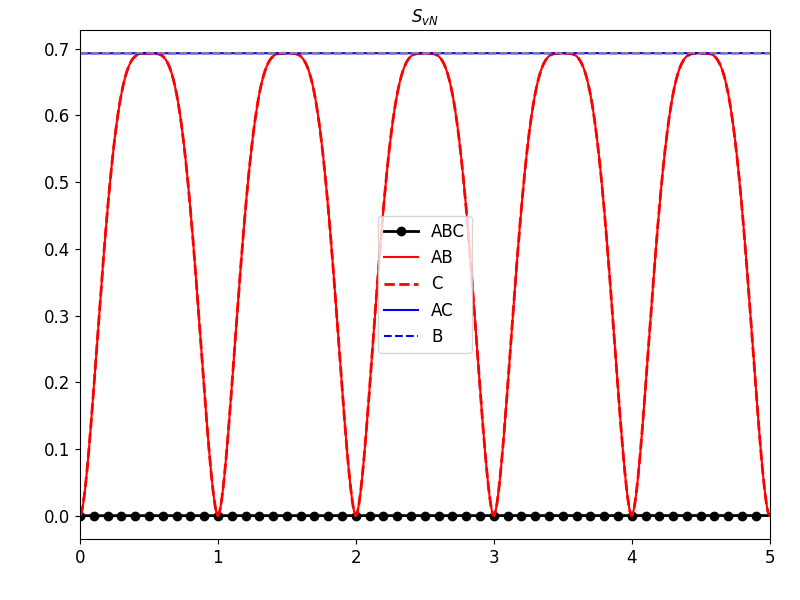
\includegraphics[width=\textwidth]{figuras/ch4/d eg0+ din svn d=0.png}
        \caption{}
        \label{fig4:dinamica svn eg0 sim resonante}
    \end{subfigure}
    \caption{\textcolor{red}{labels, ticks y legens chiquitos. unificar colores}Panel (a):Dinámica poblacional para el caso resonante $\Delta=0$ con el estado inicial entrelazado $\ket{\psi_0}=(\ket{eg0} + \ket{ge0})/\sqrt{2}$. Panel (b):Entropía de von Neuman del sistema total (negro con puntos), y de diferentes subsistemas. En rojo se muestra la entropía del sistema habiendo trazado parcialmente sobre la cavidad, y en azul habiendo trazado parcialmente sobre el átomo B.}
    \label{fig4:dinamica eg0 sim resonante}
\end{figure}

En la figura \ref{fig4:dinamica pob eg0 sim resonante} se muestran las poblaciones y las coherencias correspondientes a la condición inicial $\ket{\psi_0}=(\ket{eg0} + \ket{ge0})/\sqrt{2}$ en el caso resonante, y en la figura \ref{fig4:dinamica svn eg0 sim resonante} se muestra la entropía de Von Neuman, en función del tiempo $t/T$ con $T=2 \pi \Omega(n,j)$  . La entropía de von Neuman es una cantidad que esta definida según:
\begin{equation}\label{eq4:entropia von neuman}
    S=-\Tr(\rho \ln \rho)=-\sum_j \lambda_j \ln \lambda_j
\end{equation}
donde $\rho$ es la matriz densidad del sistema, y $\lambda_j$ son los autovalores de la matriz densidad. La entropía de Von Neuman sirve para determinar si un estado es puro o mixto, ya que $S(\rho)=0$ representa un estado puro, y $S(\rho)=\ln(N)$ representa un estado máximamente mixto, donde $N$ es la dimensión del espacio de Hilbert.
Vemos como el estado $\ket{ge0}$ no evoluciona, ya que en este caso, el átomo B contiene la única excitación y esta aislado. Pero la otra parte, si que evoluciona. Vemos la presencia de las mismas oscilaciones coherentes entre los estados $\ket{eg0}$ y $\ket{gg1}$. La diferencia principal es que en esta caso, el estado de los subsistemas es mixto. Esto se observa claramente en el gráfico de la entropía, pero también se puede deducir este comportamiento desde la figura \ref{fig4:dinamica pob eg0 sim resonante}, ya que a $t/T=0.5$, tenemos el estado $\ket{\psi(T/2)}=\ket{g}_A\otimes(\ket{e_B0_C}+\ket{g_B1_C})/\sqrt{2}$, que es separable solo en el átomo A, y los otros dos están totalmente entrelazados, y por lo tanto al tomar traza parcial tal que el átomo B y la cavidad estén separadas, este estado es máximamente mixto. Vemos como el entrelazamiento entre la cavidad y el átomo B, que están totalmente aislados, evoluciona indirectamente por medio del átomo A, y paradójicamente este queda desentrelazado del sistema para tiempos $t=(k-1/2)T\; ; \; k \in \mathbb{N}$. En este punto notamos algo muy importante, y es que la entropía de von Neuman solo sirve para estados puros. Cuando $t=0$, la entropía del subsistema AB es 0, porque es un estado puro, y esta máximamente entrelazado. Pero al evolucionar, el subsistema AB se hace mixto, y como se observa en la linea azul, la entropía del átomo B es siempre $\log 2$, que según la interpretación de la entropía de von Neuman es que esta siempre máximamente entrelazado. Este no es al caso, y la descripción falla porque el estado AB no es puro.

Entonces, ya que el entrelazamiento es un recurso muy importante y estudiado para las información cuántica, es necesario introducir una medida de entrelazamiento, para poder estudiarlo en este tipo de situaciones. Si bien la entropía de Von Neuman es útil en el caso de estados puros, cuando tenemos estados mixtos como se vio recién, o en el caso de tener un sistema abierto, esta medida ya no sirve. Una de las medidas mas utilizadas y con mayor aplicación es el \textit{Entanglement of Formation} ($E_F$) \cite{an intro to entanglement measures}, que coincide con la entropía de von Neuman para estados puros, y sirve para estados mixtos. El $E_F$ esta definido como
\begin{equation}
    E_F(\rho)=\text{inf}\left( \sum_i p_i E(\ketbra{\psi_i}{\psi_i}) : \rho = \sum_i p_i\ketbra{\psi_i}{\psi_i}\right)
\end{equation}
Esta medida representa el entrelazamiento promedio mínimo entre todas las posibles descomposiciones puras de $\rho$, donde $E(\ketbra{\psi_i}{\psi_i})=S(\tr_B{\ketbra{\psi_i}{\psi_i}})$ es la entropía de von Neuman, que es la medida que se utiliza para estados puros. Esta definición es general, pero en el caso presente, nos sirve una simplificación de esta medida que se obtiene si se estudia el entrelazamiento entre dos qu-bits, como lo son los átomos A y B. Esta medida es la concurrencia, y esta definida como
\begin{equation}
    C(\rho)=\text{max}\{0,\lambda_1-\lambda_2-\lambda_3-\lambda_4\}
    \label{ec4:concurrencia}
\end{equation}
donde los $\lambda_i$ son las raíces de los autovalores, en orden decreciente, de la matriz $\rho\sigma_y\otimes\sigma_y\rho^*\sigma_y\otimes\sigma_y$, donde $\rho*$ es el conjugado (sin transponer) de $\rho$. La concurrencia y la entropía de formación $E_F$ están relacionadas, y la concurrencia obtiene su interpretación a través de esta. Un estado máximamente entrelazado tiene $C(\rho)=1$ y un estado separable $C(\rho)=0$. 


\begin{figure}[H]
    \begin{minipage}[c]{0.67\textwidth}
        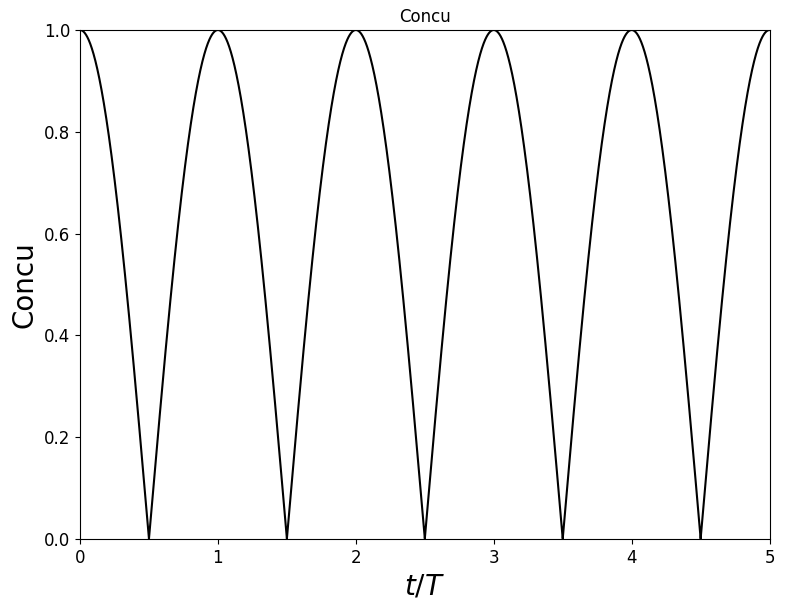
\includegraphics[width=\textwidth]{figuras/ch4/d eg0+ concu d=0.png}
    \end{minipage}\hfill
    \begin{minipage}[c]{0.3\textwidth}
    \caption{Concurrencia en el caso resonante para estado inicial $\ket{eg0}+\ket{ge0}$
         } \label{fig4:concu eg0 sim}
  \end{minipage}
\end{figure}
En la figura \ref{fig4:concu eg0 sim} se observa la concurrencia entre los átomos AB, para el caso estudiado anteriormente. Como era de esperar, a $t=0$ el estado es máximamente entrelazado, y luego el entrelazamiento se pierde a $t=T/2$, donde el átomo B esta entrelazada con la cavidad. 

\subsection{Interacción átomo-átomo}

El siguiente paso es analizar el rol de las interacciones entre los átomos, aun manteniendo el apantallamiento $\alpha=0$. Para esto, se sigue utilizando las mismas condiciones iniciales y el átomo B seguirá sin interactuar con la cavidad, pero se considera ahora que la interacción entre átomos dadas por los parámetros $k$ y $J$ ahora serán distintos de cero. Para comenzar, en la figura \ref{fig4:k eg0 abc} se observa la evolución temporal para el estado inicial $\ket{\psi_0}=\ket{eg0}$, con $\Delta = 0$, $J=0$ pero $k=0.1g$. Recordemos que $k$ es la intensidad de la interacción $\sigma^{(1)}_+\sigma^{(2)}_-+\text{c.c.}$ (ver \ref{eq4:H}).

\begin{figure}[h]
    \begin{minipage}[c]{0.67\textwidth}
        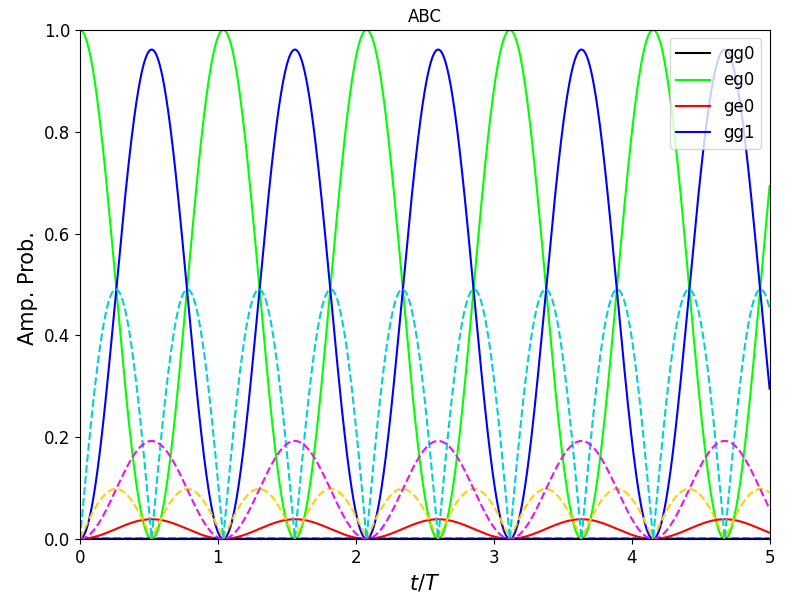
\includegraphics[width=\textwidth]{figuras/ch4/k eg0 ABC.png}
    \end{minipage}\hfill
    \begin{minipage}[c]{0.3\textwidth}
    \caption{Dinámica poblacional para la condición inicial $\ket{\psi_0}=\ket{eg0}$, para los parámetros $\Delta=0$, $J=0$ y $k=0.1g$. Las lineas solidas se corresponden con las poblaciones de la matriz densidad total del sistema; en azul la probabilidad de encontrar al estado en el estado $\ket{gg1}$, en verde en $\ket{eg0}$, en rojo $\ket{ge0}$, y en negro $\ket{gg0}$. Las lineas rayadas son las coherencias entre estas poblaciones, la violeta entre $\ket{gg1}$ y $\ket{ge0}$, la celeste entre $\ket{eg0}$ y $\ket{gg1}$ y la amarilla entre $\ket{eg0}$ y $\ket{gg1}$.
         } \label{fig4:k eg0 abc}
  \end{minipage}
\end{figure}
Lo que sucede es que la excitación esta inicialmente en el átomo A, y como siempre, se observan oscilaciones entre los estados $\ket{eg0}$ y $\ket{gg1}$, la diferencia es que al haber interacciones entre los átomos, ahora la excitación inicial que esta en el átomo A, sufre dos procesos diferentes, primero la oscilación, y ademas, la interacción con el átomo B. Al tener la excitación el átomo A, una parte de esta se va hacia la cavidad, y la otra hacia el átomo B, excitándolo parcialmente. La amplitud de la oscilación depende de la intensidad de la interacción $k$. Si nos concentramos en la curva roja, vemos que su pendiente crece mientras que la probabilidad de $\ket{eg0}$ es mayor a la de $\ket{gg1}$, luego la amplitud crece, pero de manera desacelerada, hasta que la probabilidad del estado $\ket{eg0}$ es nula. En ese momento, ya no hay excitación que pasar del átomo A al B, y el proceso se revierte. Antes de analizar el entrelazamiento entre los átomos, se observa en la figura \ref{fig4:k eg0 sim abc} la dinámica para los mismos parámetros, pero para la condición inicial entrelazada $\ket{\psi_0}=(\ket{eg0}+\ket{ge0})/\sqrt{2}$:
\begin{figure}[h]
    \begin{minipage}[c]{0.67\textwidth}
        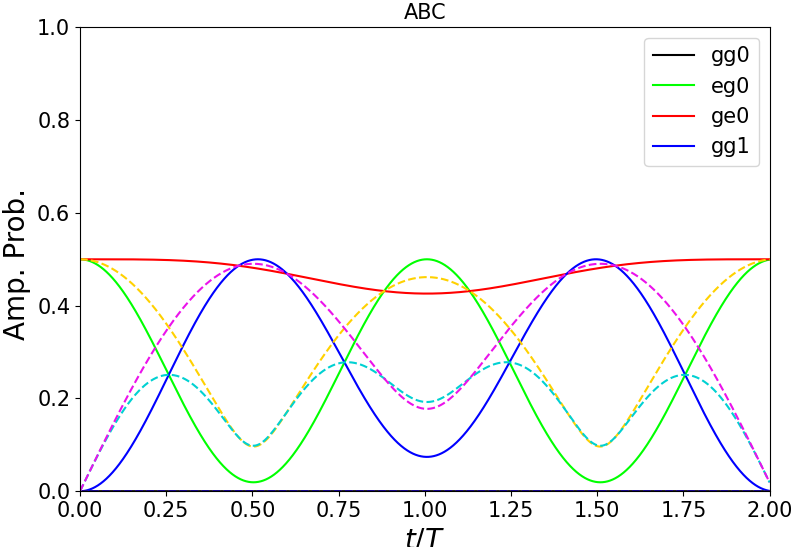
\includegraphics[width=\textwidth]{figuras/ch4/k eg0+ ABC.png}
    \end{minipage}\hfill
    \begin{minipage}[c]{0.3\textwidth}
    \caption{Dinámica poblacional para la condición inicial $\ket{\psi_0}=\ket{eg0+ge0}$, para los parámetros $\Delta=0$, $J=0$ y $k=0.1g$. Las coherencias y poblaciones tienen los mismos colores que la figura anterior \ref{fig4:k eg0 abc}
         } \label{fig4:k eg0 sim abc}
  \end{minipage}
\end{figure}
La dinámica en este caso presenta oscilaciones en la población de $\ket{ge0}$ con un periodo dos veces mas grande. Esto se debe a una \"pelea\" entre los estados $\ket{eg0}$ y $\ket{ge0}$, ya que tienen las excitaciones en diferentes átomos. Inicialmente, como los estados están entrelazados, no esta bien definido en cual de los dos átomos esta la excitación, entonces la interacción $k$ se anula y vemos que tiene pendiente 0. Entonces la dinámica inicial es igual que para $k=0$ y comienza a oscilar. Apenas baja la curva verde, la probabilidad de encontrar la excitación en el átomo B es mayor que la del átomo A, entonces lo que sucede es que el átomo B comienza a perder esta excitación y se la da lentamente al átomo A, y por lo tanto la oscilación del estado $\ket{eg0}$ no llega a tener amplitud nula en $t/T=0.5$. Luego, la evolución sigue su curso oscilante, y al llegar a $t=T$, vemos que la probabilidad de encontrar la excitación en el átomo A es mayor, y por lo tanto comienza a revertirse la situación, hasta completar el ciclo para $t=2T$. \textcolor{red}{no es exacto pq puse algo mal en el codigo, pero ahora esta corregido y da bien. tengo que cambiar estas imagenes.} 

El entrelazamiento entre los átomos se analiza utilizando la concurrencia, como se muestra en la figura \ref{fig4:concu k}, donde \ref{fig4:concu k eg0} muestra la condición inicial separable $\ket{eg0}$, y \ref{fig4:concu k eg0 sim} el entrelazamiento para la condición inicial entrelazada $\ket{eg0+ge0}$. 
\begin{figure}[h]
    \centering
    \begin{subfigure}{0.49\textwidth}
        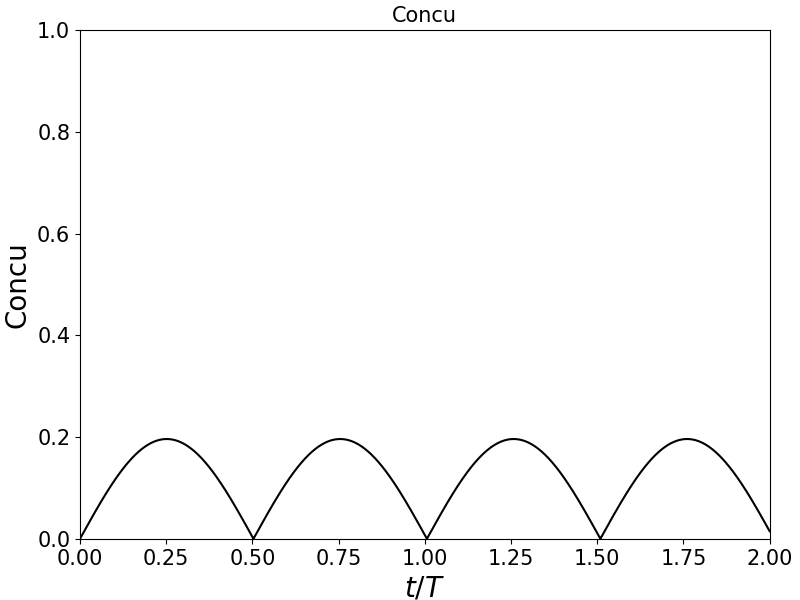
\includegraphics[width=\textwidth]{figuras/ch4/k eg0 concu.png}
        \caption{$\ket{eg0}$}
        \label{fig4:concu k eg0}
    \end{subfigure}
    \hfill
    \begin{subfigure}{0.49\textwidth}
        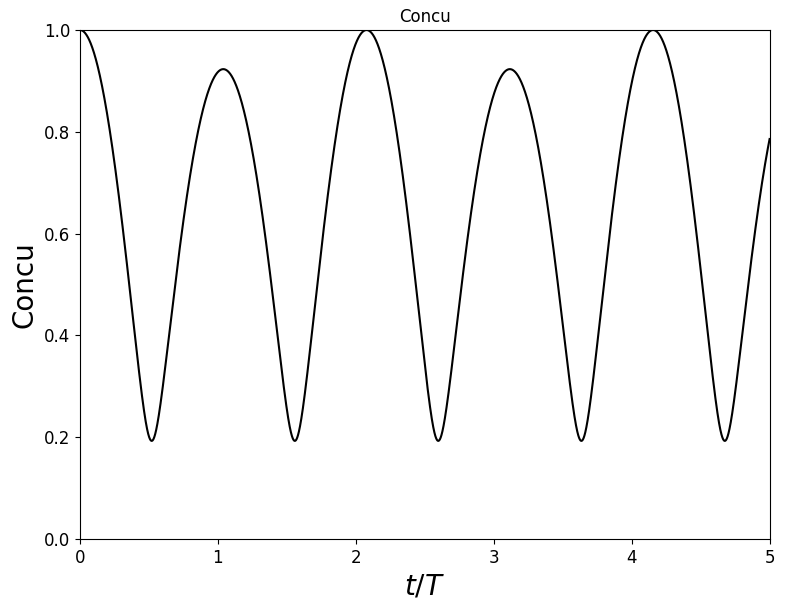
\includegraphics[width=\textwidth]{figuras/ch4/k eg0+ concu.png}
        \caption{$\ket{eg0+ge0}$}
        \label{fig4:concu k eg0 sim}
    \end{subfigure}
    \caption{\textcolor{red}{rehacer por labels chiquitos}Dinámica de entrelazamiento para $\Delta=0$, $J=0$ y $k=0.1g$}
    \label{fig4:concu k}
\end{figure}

Ahora vamos a ver $k=0$ y $J\neq 0$. En la figura \ref{fig4:j alpha0}, vemos que, si bien la dinámica es similar, los átomos no se entrelazan.

\begin{figure}[H]
    \centering
    \begin{subfigure}{0.49\textwidth}
        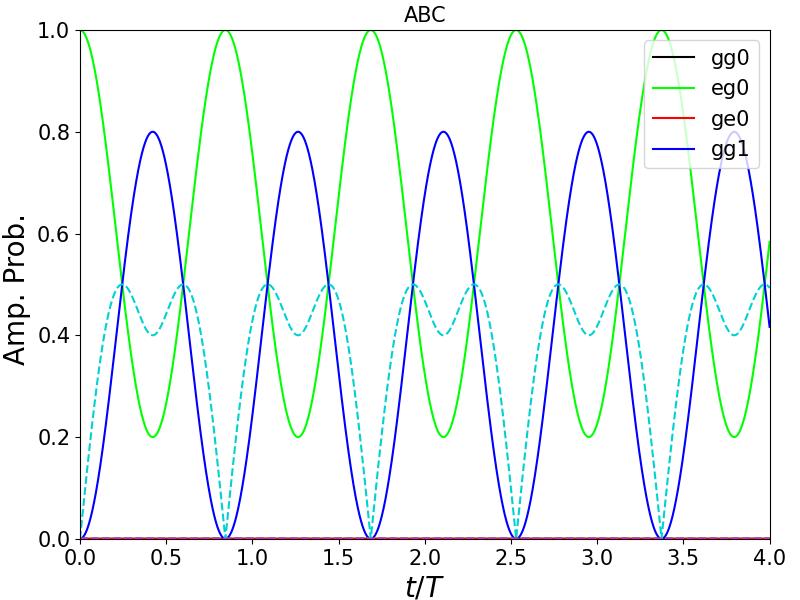
\includegraphics[width=\textwidth]{figuras/ch4/j eg0 abc.png}
        \caption{$\ket{eg0}$ Poblaciones}
        \label{fig4:pob j eg0}
    \end{subfigure}
    \hfill
    \begin{subfigure}{0.49\textwidth}
        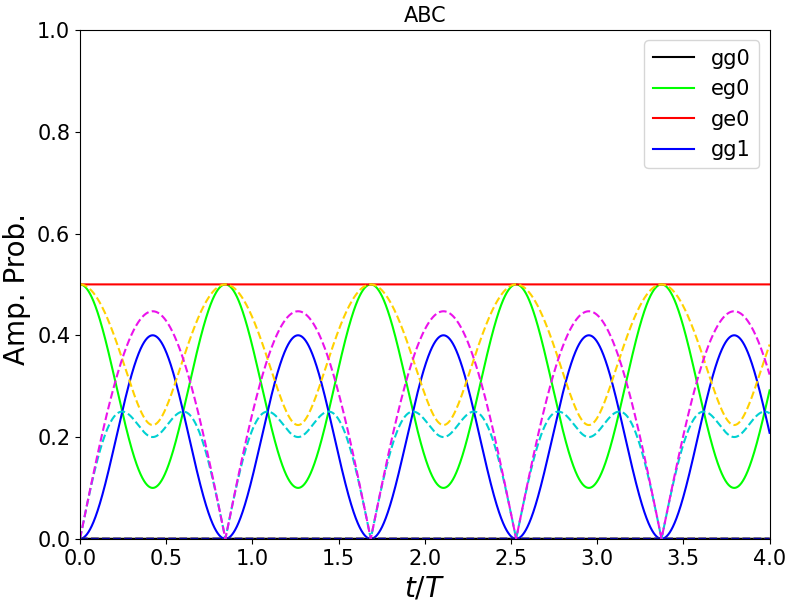
\includegraphics[width=\textwidth]{figuras/ch4/j eg0+ge0 abc.png}
        \caption{$\ket{eg0+ge0}$ Poblaciones}
        \label{fig4:pob j eg0 sim}
    \end{subfigure}
    \vfill
    \begin{subfigure}{0.49\textwidth}
        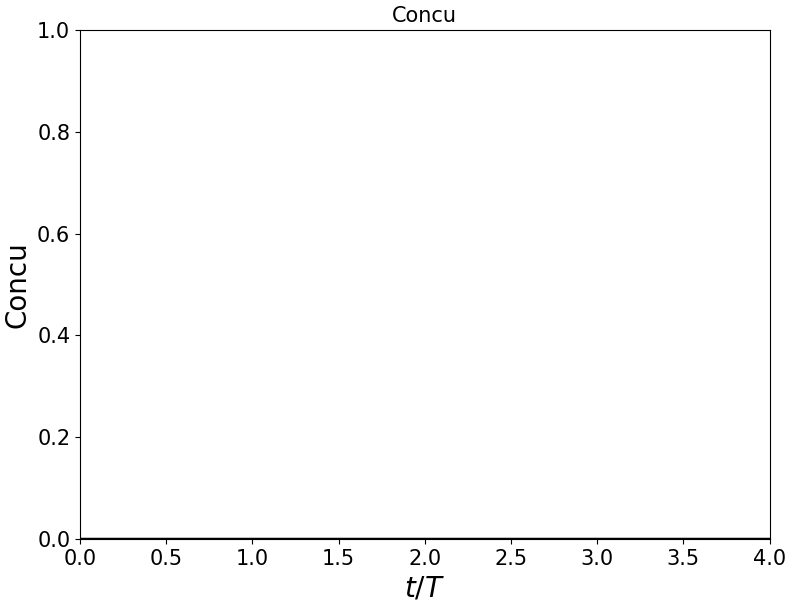
\includegraphics[width=\textwidth]{figuras/ch4/j eg0 concu.png}
        \caption{$\ket{eg0}$ Concurrencia}
        \label{fig4:pob j eg0}
    \end{subfigure}
    \hfill
    \begin{subfigure}{0.49\textwidth}
        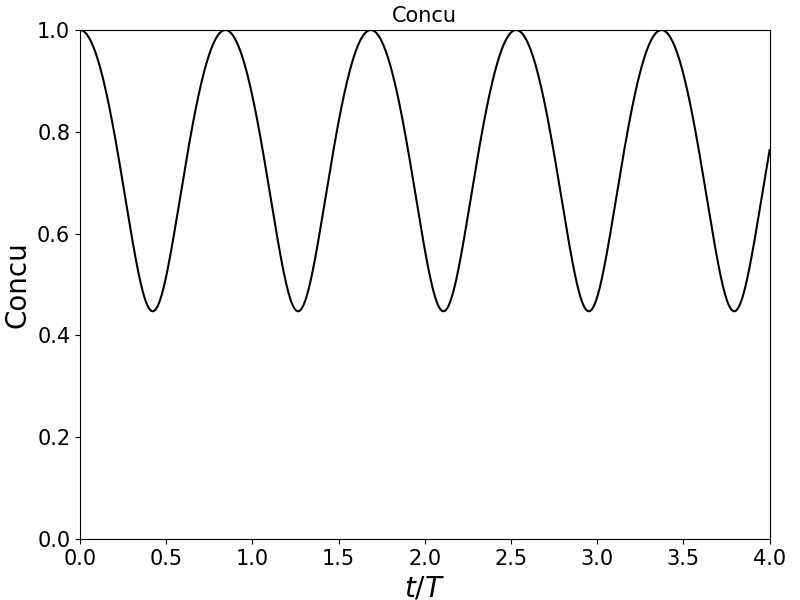
\includegraphics[width=\textwidth]{figuras/ch4/j eg0+ge0 concu.png}
        \caption{$\ket{eg0+ge0}$ Concurrencia}
        \label{fig4:pob j eg0 sim}
    \end{subfigure}
    \caption{$\Delta=0$, $J=0.5g$ y $k=0$}
    \label{fig4:j alpha0}
\end{figure}
Vemos que la diferencia principal entre la interacción tipo Isign ($J\sigma_z^{(1)}\sigma_z^{(2)}$) y la dipolar ($k\sigma_+^{(1)}\sigma_-^{(2)}+\text{c.c.}$), es que el segundo parece entrelazar los átomos, ya que en el primer caso, el efecto es separar los niveles de energía, pero en el segundo no solo eso, sino que también pasa excitaciones de un atomo al otro. Si bien esto nos sirve para entender intuitivamente el efecto, el problema de este análisis es que estamos asumiendo cosas no físicas mediante el apantallamiento y la asimetría que imponemos entre los dos átomos. Esto, lleva a estos análisis que en realidad no son correctos, ya que si miramos el Hamiltoniano del sistema sin apantallamiento \ref{eq4:H}, donde usamos la base con estados simétricos y antisimetricos \ref{ec4:base}, el efecto de ambos parámetros debería ser el mismo, ya que solo aparecen en la diagonal principal. Si bien la interacción $J$ actúa sobre todos los estados, y el $k$ solamente solo sobre los $\ket{egn\pm gen}$, su principal función es separar las energías de los estados de la base.
Entonces sera necesario retomar este análisis sin apantallamiento y con la base \ref{ec4:base}.
\subsection{Medio Kerr}

Ahora nos concentramos en el efecto del medio Kerr. Para esto, apagamos las interacciones interatómicas $k=J=0$, y ahora se modifica el medio a través del parámetro $\chi$. 
\begin{figure}[h]
    \centering
    \begin{subfigure}{0.49\textwidth}
        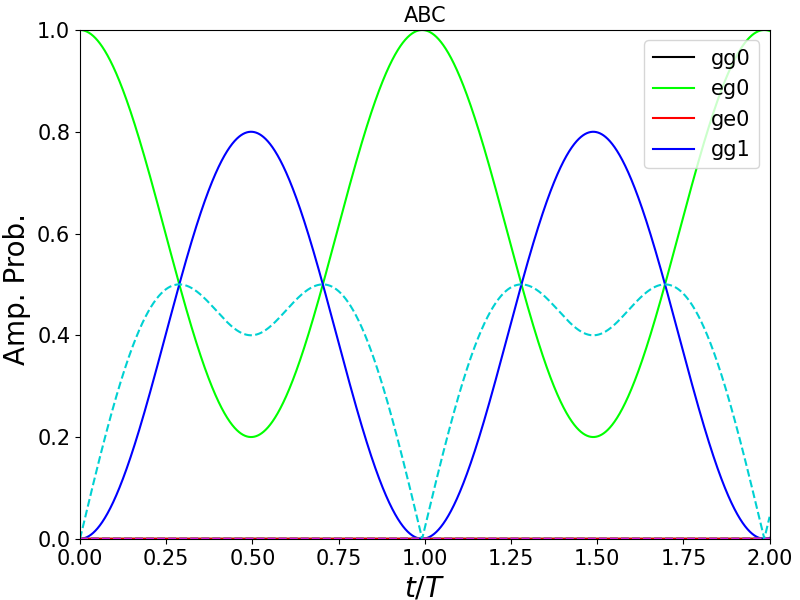
\includegraphics[width=\textwidth]{figuras/ch4/x eg0 abc.png}
        \caption{$\ket{eg0}$}
        \label{fig4:pob x eg0}
    \end{subfigure}
    \hfill
    \begin{subfigure}{0.49\textwidth}
        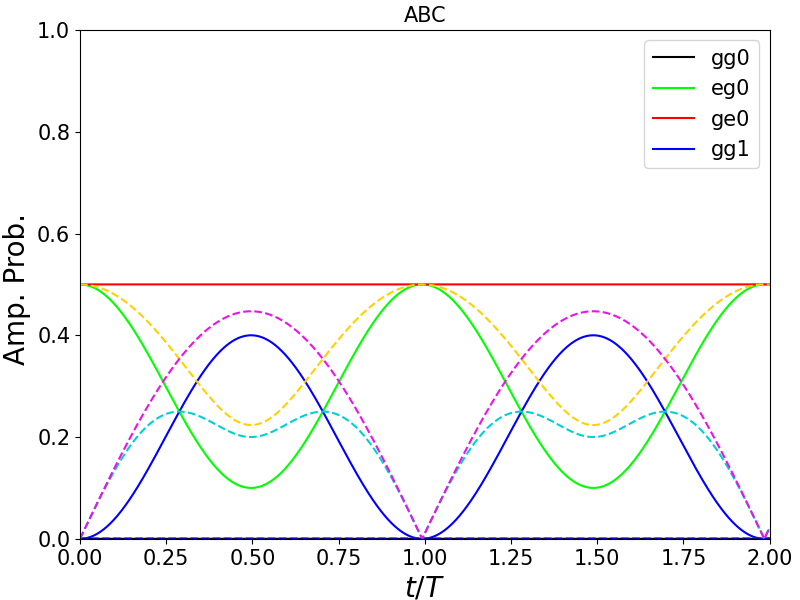
\includegraphics[width=\textwidth]{figuras/ch4/x eg0+ abc.png}
        \caption{$\ket{eg0+ge0}$}
        \label{fig4:pob x eg0 sim}
    \end{subfigure}
    \caption{Dinámica de poblaciones para $x=g$}
    \label{fig4:pob x}
\end{figure}

Al igual que en el caso de 1 átomo, se puede observar en las ecuaciones \ref{ec4:autoenergias} y \ref{ec4:parametros solucion}, la frecuencia depende del medio. En la figura \ref{fig4:pob x} el tiempo esta normalizado con la frecuencia, entonces no se nota el cambio. Pero lo que es necesario analizar, es como las oscilaciones no son totalmente coherentes, en el sentido de que la probabilidad del estado $\ket{gg1}$ nunca alcanza la amplitud inicial de la oscilación, como en el caso de $\chi=0$. Esto se debe a que el aumento de $\chi$ hace que las energías de ambos estados se separen, y por lo tanto hace que las transiciones entre los estados sea menos probable. Este comportamiento también se observa si el estado inicial se toma como $\ket{gg1}$. Es lógico estudiar el entrelazamiento en este caso. En la figura \ref{fig4:concu x} se muestran las concurrencias para ambas condiciones iniciales. Es interesante comparar la figura \ref{fig4:concu x eg0 sim} con la figura en el caso de $\chi=0$ para esta misma condición inicial, la figura \ref{fig4:concu eg0 sim}. En principio se puede pensar que el medio no lineal rompe con el entrelazamiento del sistema, pero como se ve al comparar estas figuras, la interpretación correcta es que el medio no hace mas que ralentizar el comportamiento preexistente de la cavidad, ya que en este caso, no destruye el entrelazamiento, sino que lo conserva por virtud de haber ralentizado las amplitudes de oscilación entre los dos estados dinámicos.
\begin{figure}[h]
    \centering
    \begin{subfigure}{0.49\textwidth}
        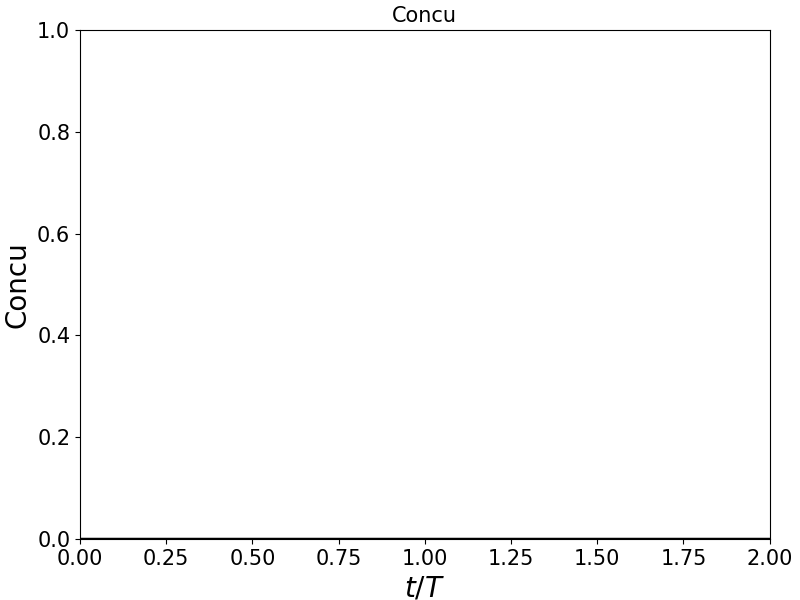
\includegraphics[width=\textwidth]{figuras/ch4/x eg0 concu.png}
        \caption{$\ket{eg0}$}
        \label{fig4:concu x eg0}
    \end{subfigure}
    \hfill
    \begin{subfigure}{0.49\textwidth}
        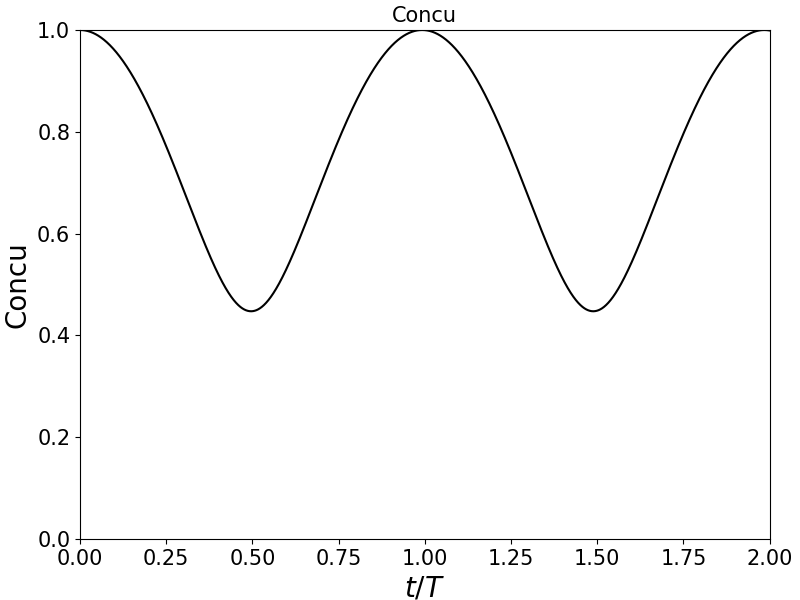
\includegraphics[width=\textwidth]{figuras/ch4/x eg0+ concu.png}
        \caption{$\ket{eg0+ge0}$}
        \label{fig4:concu x eg0 sim}
    \end{subfigure}
    \caption{Dinámica de entrelazamiento para $x=g$}
    \label{fig4:concu x}
\end{figure}
Cambien se puede intentar de recuperar el comportamiento visto en el modelo de 1 átomo, que el medio Kerr no es mas que un desplazamiento lateral en las frecuencias, ademas de modificar las amplitudes. Para esto se realiza otra evolución para $\chi=\Delta=\frac{g}{2}$, y se compara con el caso en que $\chi=\Delta=0$
\begin{figure}[h]
    \centering
    \begin{subfigure}{0.49\textwidth}
        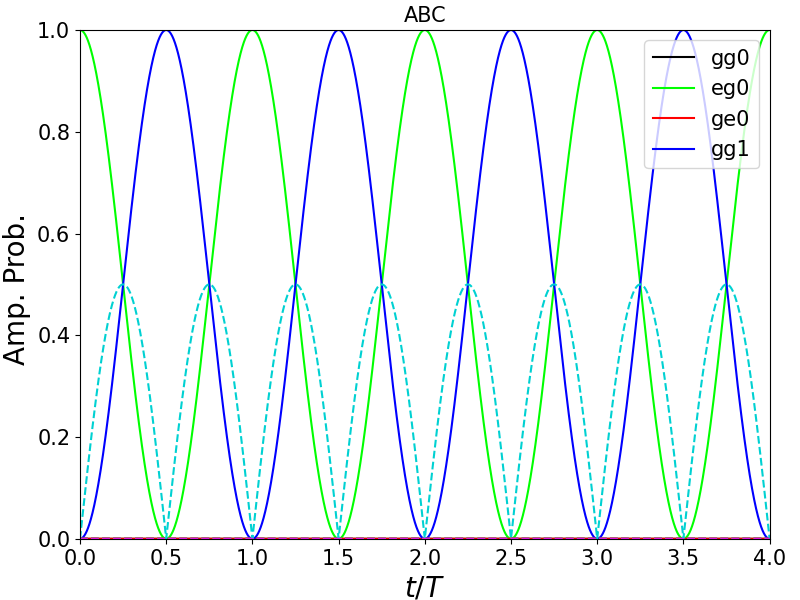
\includegraphics[width=\textwidth]{figuras/ch4/d=x=0 eg0 abc.png}
        \caption{$\Delta=\chi=0$}
        \label{fig4:comparacion kerr pob 1}
    \end{subfigure}
    \hfill
    \begin{subfigure}{0.49\textwidth}
        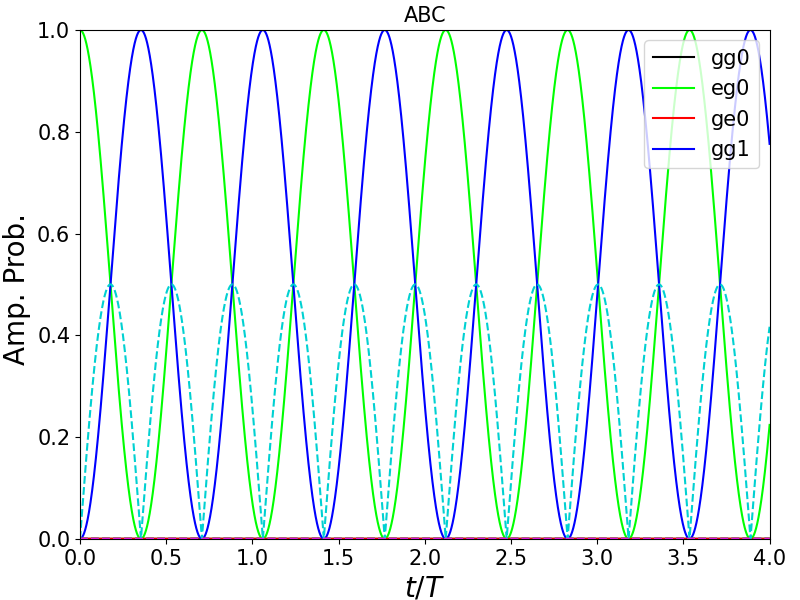
\includegraphics[width=\textwidth]{figuras/ch4/d=x=0.5 eg0 abc.png}
        \caption{$\Delta=\chi=0.5g$}
        \label{fig4:comparacion ker pob 2}
    \end{subfigure}
    \caption{Dinámica de entrelazamiento para $x=g$}
    \label{fig4:comparacion d vs x}
\end{figure}
Vemos como se anula el efecto del medio, y la dinámica es la misma pero con un cambio en la frecuencia. Al igual que antes, aumenta la frecuencia

\subsection{Batidos}

Al complejizar el problema, comienzan a aparecer batidos, comportamiento que se atribuye a la modulación de dos procesos simultáneos. Por ejemplo, si observamos la evolución temporal con $\chi\neq0$ y $k\neq0$, entonces el primero disminuye la amplitud de oscilación de, los estados con mayor cantidad de fotones en la cavidad, que dentro del subespacio $N$ la jerarquía del medio sera favorecer a los estados $\ket{eg,N-1}$ y $\ket{ge,N-1}$ por sobre el $\ket{ggN}$. Por el contrario, se observo que en esta situación, el termino de interacción entre los átomos disminuye la amplitud del estado $\ket{ggN}$ como se vio en la sección anterior. Por lo tanto, si tenemos dos procesos que están en juego y sus efectos son similares, entonces es esperable que se observen oscilaciones moduladas. No vale la pena mostrar la dinámica de las poblaciones, porque no se pueden sacar conclusiones muy importantes, pero si podemos observar la trayectoria en la esfera de bloch, para dar una idea de la complejidad de la evolución.

\section{Dinámica sin apantallamiento}

Al sacar el apantallamiento, es necesario utilizar la base mencionada anteriormente \ref{ec4:base}, ya que los átomos son indistinguibles y esta base es mas apropiada. Ademas, el Hamiltoniano desacopla los estados antisimetricos, facilitando la solución. Por lo tanto, se procede a estudiar la dinámica sacando el apantallamiento. Lo que nos interesa estudiar es el entrelazamiento entre las diferentes partes del sistema, y su dependencia con los parámetros. 

\subsection{Dinámica con disipación}

Lo primero que hay que mirar es la dependencia de la dinámica con el régimen de acoplamiento, esperamos un comportamiento igual al del caso de un átomo \ref{sec3:regimen acoplamiento}. Recordemos que el régimen de acoplamiento fuerte (SC) es el caso en donde la interacción entre cavidad y átomos es mayor a la interacción entre sistema y entorno.
\begin{figure}[h]
    \centering
    \begin{subfigure}{0.7\textwidth}
        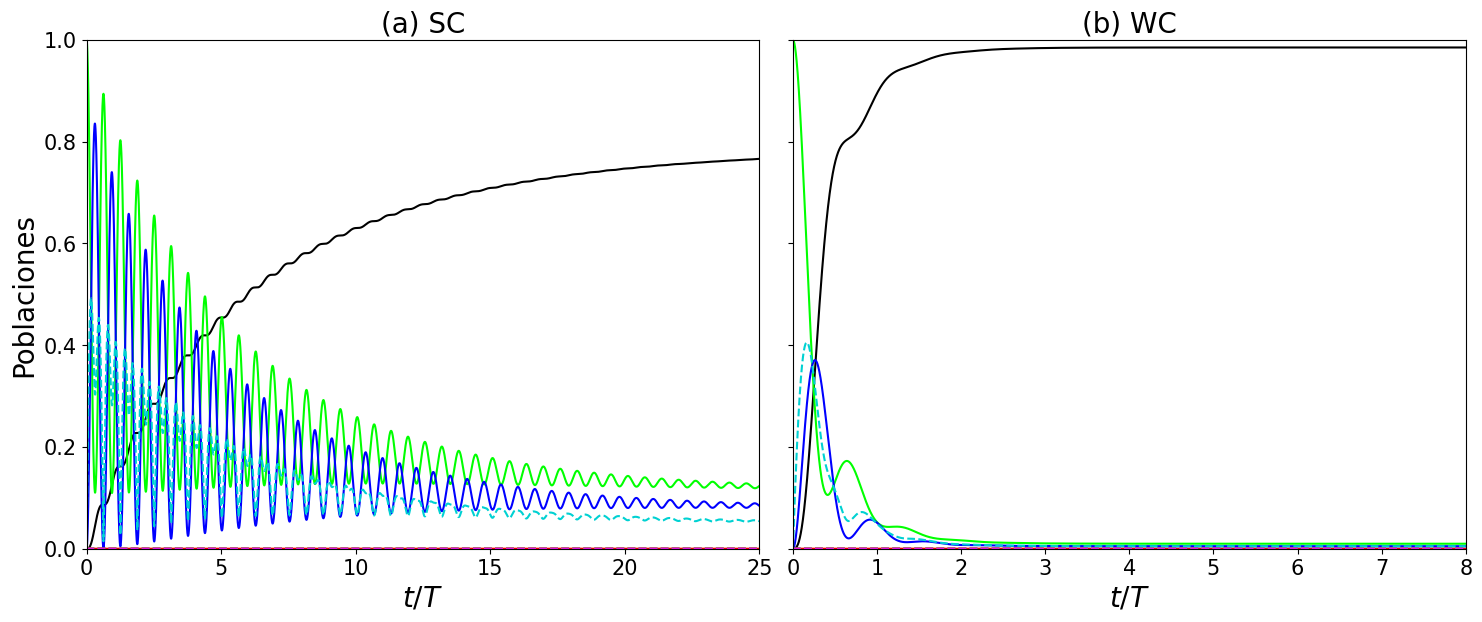
\includegraphics[width=\textwidth]{figuras/ch4/sc vs wc eg0 sim j0.5.png}
        \caption{$\ket{eg0+ge0}$. $\Delta=\chi=k=0$, $J=0.5g$}
        \label{fig4:acoplamiento eg0 sim}
    \end{subfigure}
    \vfill
    \begin{subfigure}{0.7\textwidth}
        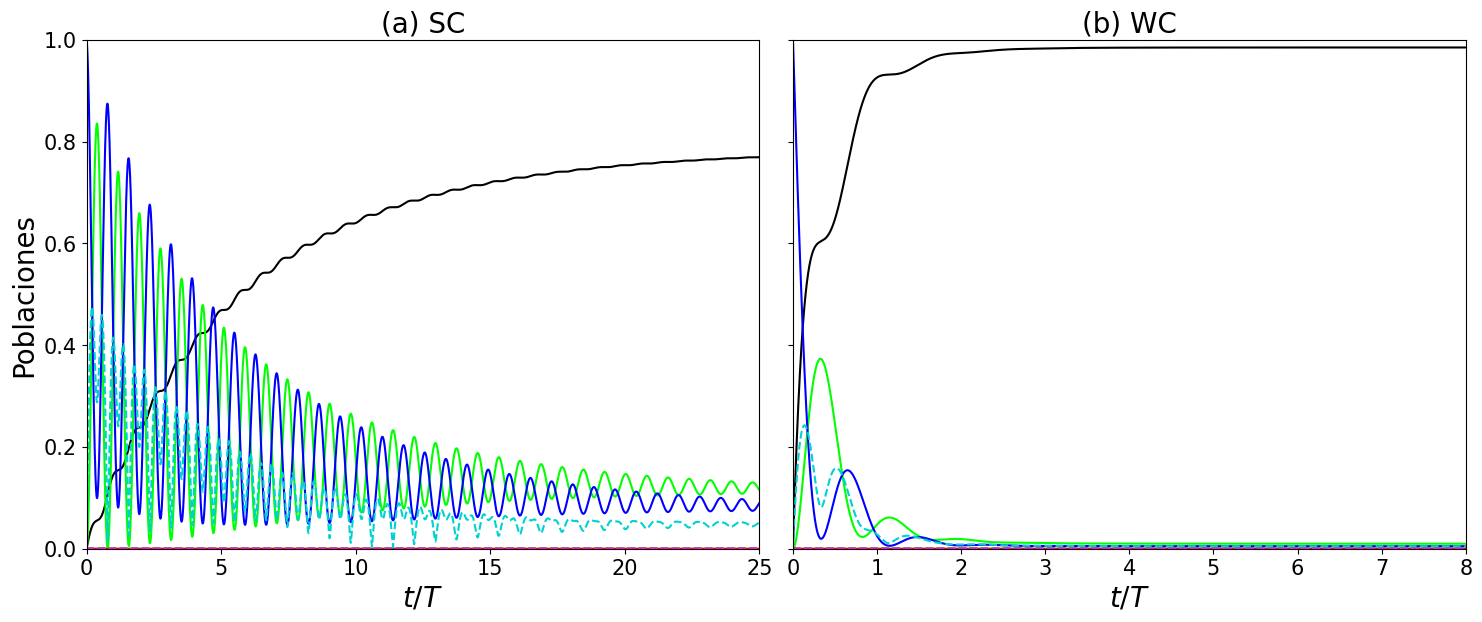
\includegraphics[width=\textwidth]{figuras/ch4/sc vs wc gg1 k=0.5.png}
        \caption{$\ket{gg1}$. $\Delta=\chi=J=0$, $k=0.5g$ }
        \label{fig4:acoplamiento gg1}
    \end{subfigure}
    \caption{Dependencia de las poblaciones con el régimen de acoplamiento, para $\Delta=J=\chi=0$ y $k=0.5g$, y para dos condiciones iniciales diferentes.}
    \label{fig4:regimen acoplamiento}
\end{figure}
En  la figura \ref{fig4:regimen acoplamiento} se  muestran las coherencias y las poblaciones, como se esperaba, estas tienen el mismo comportamiento que en el caso de 1 átomo. Notablemente, se puede ver el efecto de la interacción entre los átomos, como se separan las energías inicialmente las oscilaciones no logran la inversión total de población, solo una inversión parcial, y a tiempo largos la disipación hace que se tenga una mayor probabilidad de encontrar al sistema en el estado $\ket{eg0+ge0}$ ya que tiene menor energía. Eventualmente alcanza su estado estacionario. Lo que se recupera, ahora que ya no hay apantallamiento, es que ambos tipos de interacción ($J$ y $k$) generan entrelazamiento. Como es de esperarse, en ambos casos la concurrencia es oscilatoria por la naturaleza oscilante del problema, pero ahora, como el estado al que oscila

Nuevamente, nos concentraremos en el régimen SC. Si bien hasta ahora nos concentramos en estados con 1 excitación, y es interesante por sus implicancias y similitudes al modelo de 1 átomo, considerar estados con mayor cantidad de excitaciones hace a la riqueza del problema. Si solo consideramos $N=1$, tenemos 3 estados en el subespacio, de los cuales uno es el estado antisimetrico $\ket{eg0-ge0}$, que esta desconectado de los otros estados, y por lo tanto efectivamente se tiene un modelo de Jaynes-Cummings normal. Si vamos a $N=2$, ahora tenemos 4 estados en el subespacio, y 3 son relevantes. Por lo tanto, ahora veremos cuales son los efectos de las interacciones y la dinámica para estados iniciales en el subespacio de $N=2$. Para mantener el paralelismo, comenzaremos con el estado $\ket{eg1+ge1}$, pero como se vera, las condiciones iniciales cambian totalmente la dinámica de entrelazamiento del sistema. La enorme cantidad de posibilidades para elegir condiciones iniciales, hace que estudiar todos sea imposible, así que nos concentraremos en algunos.
Al tener 3 estados dinámicamente relevantes, tenemos 3 autoestados con sus respectivas autoenergías, y por lo tanto tenemos 3 frecuencias que compiten entre si, y son las 3 frecuencias de Rabi del sistema:
\begin{equation}
    \begin{aligned}
        \Omega^{(n)}_{12} &= E^{(n)}_2-E^{(n)}_1 \\
        \Omega^{(n)}_{23} &=E^{(n)}_3-E^{(n)}_2 \\
        \Omega^{(n)}_{31} &= E^{(n)}_1-E^{(n)}_3         
    \end{aligned}
    \label{ec4:frecuencias de rabi}
\end{equation}
Estas frecuencias se muestran en función del detunning $\Delta$ y para diferentes valores de $\chi$ y de $k-J$ en la figura \ref{fig4:frecuencias de rabi}.
\begin{figure}
    \centering
    \begin{subfigure}{\textwidth}
        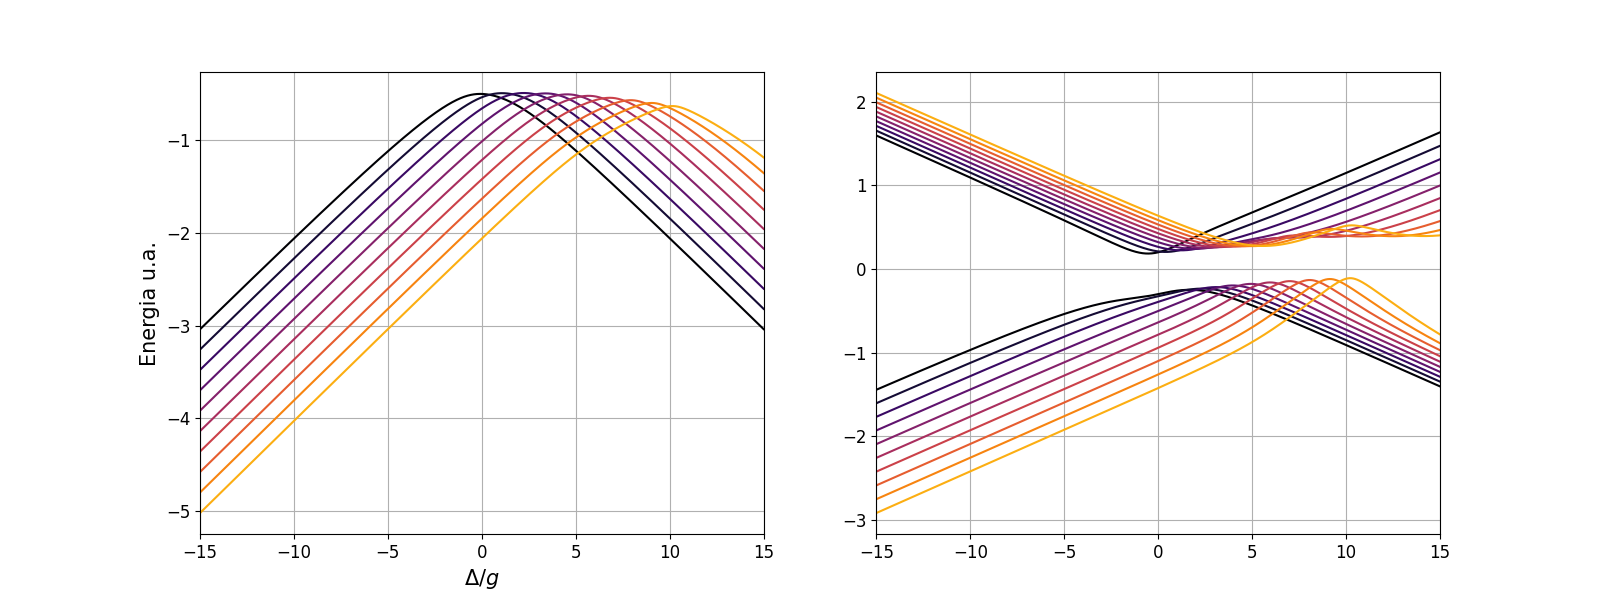
\includegraphics[width=\textwidth]{figuras/ch4/frecuencias k=0.5g chilist.png}
        \caption{Frecuencias de Rabi en función del detunning, para diferentes valores de $\chi/g\in[0,5]$ y $k-J=0.5g$. A la izquierda $\Omega_{12}$ y a la derecha $\Omega_{23}$ y $\Omega_{13}$}
        \label{fig4:rabi chi}
    \end{subfigure}
    \vfill
    \begin{subfigure}{\textwidth}
        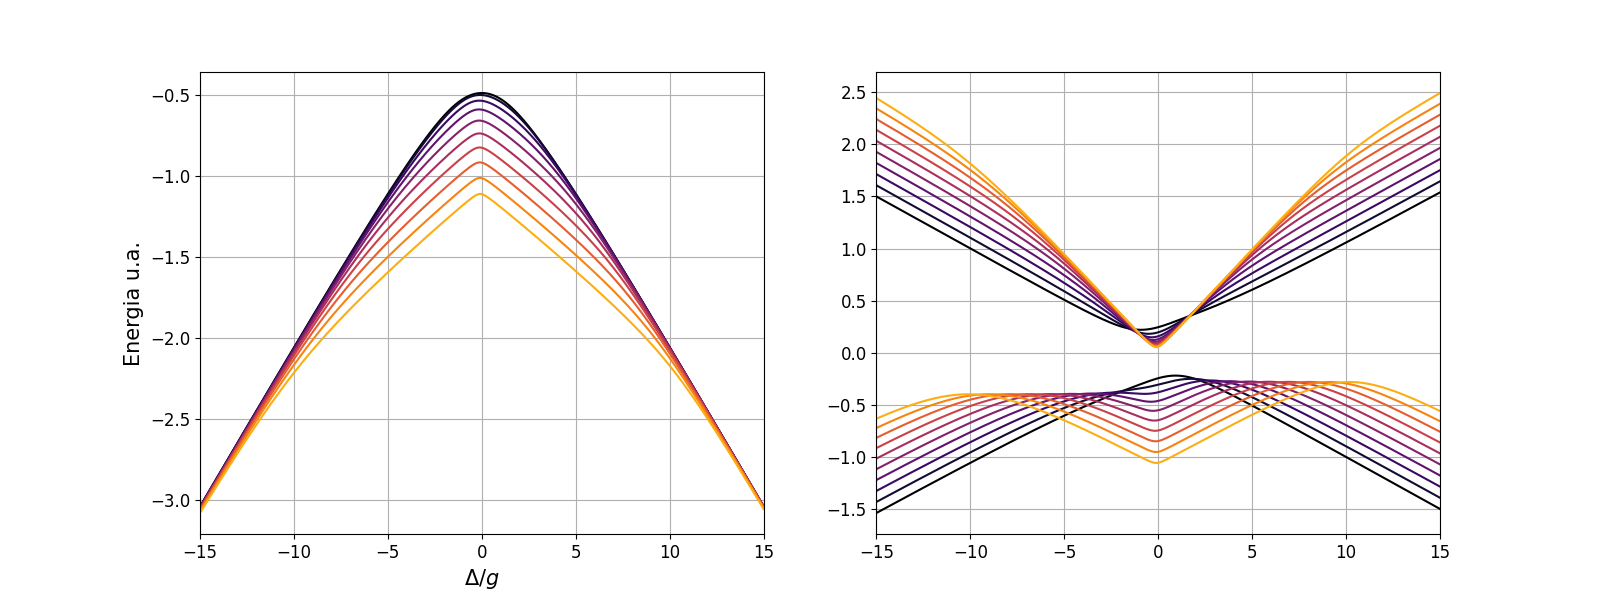
\includegraphics[width=\textwidth]{figuras/ch4/frecuencias x=0 klist.png}
        \caption{Frecuencias de Rabi en función del detunning, para diferentes valores de $k-J\in[0,5g]$ y $\chi=0$. A la izquierda $\Omega_{12}$ y a la derecha $\Omega_{23}$ y $\Omega_{13}$. Solo se muestra una de las ramas.}
        \label{fig4:rabi k}
    \end{subfigure}
    \caption{Frecuencias de Rabi en función del detunning $\Delta$ para diferentes valores de $\chi$, y $|k-J|$, donde las frecuencias de Rabi son $\Omega^{(2)}_{ij}=E^{(2)}_{j}-E^{(2)}_{i}$}
    \label{fig4:frecuencias de rabi}
\end{figure}
En esta solo se muestra una de las dos ramas (se puede tener $\pm \Omega_{ij}$) por simplicidad. Lo que podemos concluir de esto es que la frecuencia $\Omega^(2)_{12}$ se comporta de manera similar a la frecuencia de Rabi del JC de 1 átomo, que es también igual a la $\Omega^(1)$; en ambos casos la diferencia de energía presenta un máximo que se desplaza lateralmente al aumentar el parámetro $\chi$, pero presenta una sutil diferencia ya que también el máximo aumenta en valor absoluto. También se observa en la figura \ref{fig4:rabi k}, a la izquierda, como depende esta frecuencia al aumentar $k-J$, y vemos que el máximo ya no se desplaza lateralmente, sino que solo aumenta en valor absoluto. Por otro lado, en los paneles derechos, se puede analizar que sucede con las frecuencias al aumentar $\chi$ (fig. \ref{fig4:rabi chi}) y $k-J$ (fig. \ref{fig4:rabi k}). Es interesante ver como al aumentar $\chi$, se comienza a observar un máximo y mínimo local para la frecuencia $\Omega^{(2)}_{23}$ (la superior). Similarmente, pero en la rama superior, se observa este mismo comportamiento al aumentar $k-J$.

La dinámica para el caso de $N\geq2$ es muy complicada, ya que ahora se tienen 3 frecuencias diferentes, y predecir que sucede para cada combinación de parámetros y para cada condición inicial se hace muy complicado, por lo tanto, el análisis para estos casos no puede ser muy profundo. Lo que se puede distinguir es que cuando $\chi,k-J>g$, se comienzan a observar estos mínimos y máximos locales en las frecuencias, y se puede intentar de ver cual es el efecto que tiene esto en el entrelazamiento de los átomos, y también se puede observar si hay alguna relación entre los parámetros, por ejemplo como se encontró para el caso de 1 átomo (y para el subespacio de N=1) que hay una clara relación entre el detunning $\Delta$ y el medio $\chi$.

\section{Dinámica de entrelazamiento}
Para estudiar la dinámica de entrelazamiento entre los dos átomos, nos centraremos en la concurrencia ($0\leq C_{AB} \leq 1$).
\textcolor{blue}{En primer lugar consideraremos una cavidad lineal, y finalmente veremos cual es el efecto del medio Kerr sobre el entrelazamiento.}
En esta sección siempre se estudia el estado entre los dos átomos $\rho_{AB}=\tr_C\{\rho\}$, y se usa como medida de entrelazamiento la concurrencia, definida por la ecuación \ref{ec4:concurrencia}.

Lo primero que tenemos que analizar es los efectos de las interacciones entre los átomos, como ya vimos,  vamos a definir dos regímenes, que llamaremos Strong Interacting (SI) y Weak Interacting (WI), refiriéndonos a la interacción entre los átomos con respecto a la cavidad. El SI sera cuando la interacción entre los átomos es fuerte en comparación con la cavidad, es decir $k-J>g$, y WI con $k,J<g$. Ya que no se definió un limite muy claro, trabajaremos con un valor representativo de cada régimen, $k-J=0.5g$ y $k-J=2.5g$ respectivamente, ademas de utilizar un parámetro del entorno $\gamma=0.25g$. Para ilustrar la las diferencias entre condiciones iniciales, y para seguir con el paralelismo con el caso de 1 átomo, se consideraran unicamente las siguientes condiciones iniciales:
\begin{itemize}
    \item $\ket{eg0+ge0}$ para seguir el paralelismo con el JCM de 1 átomo 
    \item $\ket{eg1+ge1}$ para comparar con el anterior 
    \item $\ket{ee0+gg2}$ para ver otra condición inicial con $N=2$ 
\end{itemize}
\subsection{Dependencia con el detunning}
\subsubsection{\underline{Condicion inicial $\ket{eg0+ge0}$}}
\begin{figure}[h]
    \centering
    \begin{subfigure}{0.49\textwidth}
        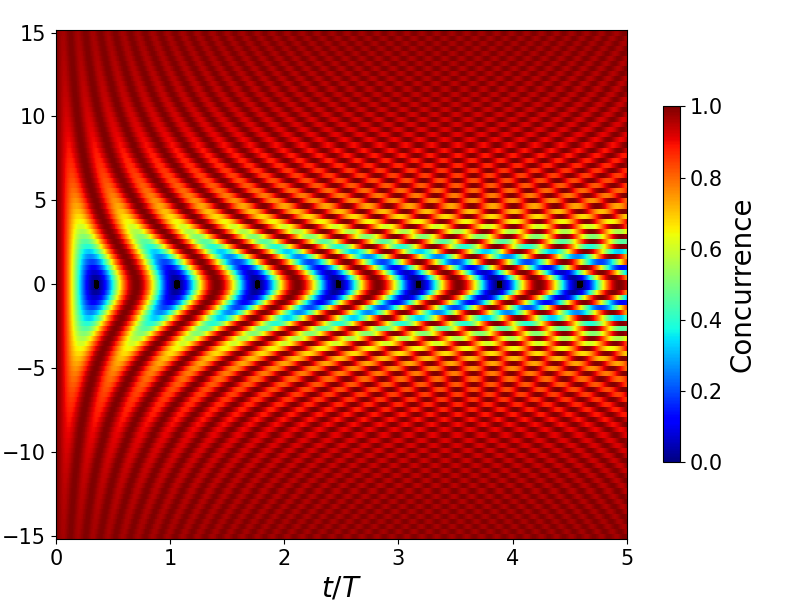
\includegraphics[width=\textwidth]{figuras/ch4/concu/delta/eg0+ge0 k=0.0g x=0.0g J=0.0g gamma=0.25g concu delta uni.png}
        \caption{Dinámica sin perdidas}
        \label{fig4:concu detunning 0 uni}
    \end{subfigure}
    \hfill
    \begin{subfigure}{0.49\textwidth}
        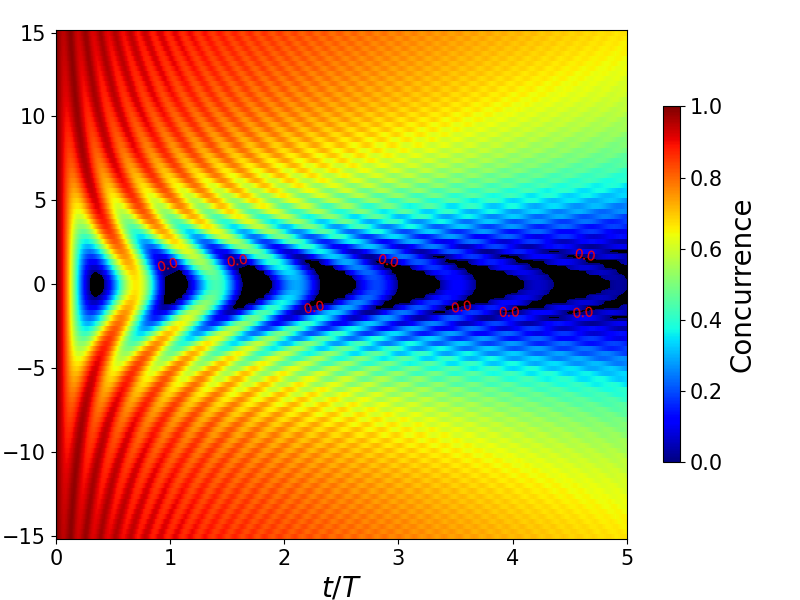
\includegraphics[width=\textwidth]{figuras/ch4/concu/delta/eg0+ge0 k=0.0g x=0.0g J=0.0g gamma=0.25g concu delta dis.png}
        \caption{Dinámica con perdidas}
        \label{fig4:concu detunning 0 dis}
    \end{subfigure}
    \caption{Dinámica de entrelazamiento para el estado inicial $\ket{eg0+ge0}$, en función del detunning, y para $\chi=k-J=0$.}
    \label{fig4:concu detunning 0}
\end{figure}
En la figura \ref{fig4:concu detunning 0} se observa la evolución de la concurrencia para la condición inicial $\ket{eg0+ge0}$, cuyo entrelazamiento entre los átomos es máximo. En el eje x es el tiempo, y en el eje y es el detunning $\Delta/g$. En el panel \ref{fig4:concu detunning 0 uni} se observa como oscila la concurrencia, llegando al cero periódicamente. Se ve como al aumentar el detunning, estas oscilaciones son cada vez de menor amplitud, y el entrelazamiento se mantiene. Ademas, la frecuencia de oscilación es cada vez mayor. Al tomar la dinámica disipativa, en el panel \ref{fig4:concu detunning 0 dis}, se observa como las oscilaciones siguen estando, pero ahora su máximo disminuye con el tiempo. Esto es de esperarse, ya que la cavidad deja escapar fotones y el estado del sistema se hace mixto. Un estado mixto ya no es entrelazado, porque no hay coherencias, entonces se observa el deterioro del entrelazamiento a medida que el tiempo avanza. Hay otros dos comportamientos notables. Por un lado, se observa como el máximo del entrelazamiento decae mas lentamente para valores mas altos del detunning, esto se debe a la naturaleza da la dinámica poblacional; al aumentar el detunning, como se vio anteriormente, uno de los efectos principales es que las oscilaciones entre los estados tienen poca amplitud, y en este caso, esto implica que si bien el estado $\ket{gg1}$ tienen amplitudes no nula, principalmente el estado del sistema esta concentrado en el estado inicial, que no sufre decoherencia por perdida de fotones, ya que no tiene fotones en la cavidad. Entonces, mientras mayor el detunning, menor la probabilidad de encontrar al sistema en el estado $\ket{gg1}$, y por lo tanto tiene pocas probabilidades de perder fotones. El otro efecto que es interesante y que aparece con frecuencia en este tipo de sistemas, es la muerte y reanimación súbita del entrelazamiento, que llamaremos SDE (Sudden Death Effect) y SBE (Sudden Birth Effect) por sus siglas en ingles. En el caso disipativo, hay marcadas zonas en negro, estas muestran como el entrelazamiento \textit{muere} durante un tiempo finito y reviven luego. Este efecto es sorprendente, ya que uno espera que las coherencias, responsables en gran medida del entrelazamiento entre átomos, decaigan asintóticamente. 

La pregunta natural que sigue es si cambiar los parametros $\chi$ y $k-J$, cambia la forma de la figura \ref{fig4:concu detunning 0}. Es de esperar que no cambie, ya que el subespacio de $N=1$ se comporta de manera sencilla, y como se concluyo anteriormente, la dependencia en los parametros $\chi$ y $k-J$ parece ser unicamente un desplazamiento de las energias de los autoestados. En la figura \ref{fig4:concu detunning 1} se muestran nuevamente la dinamica de entrelazamiento en funcion del detunning, pero ahora cambiando alguno de los parametros:

\begin{figure}[h]
    \centering
    \begin{subfigure}{0.49\textwidth}
        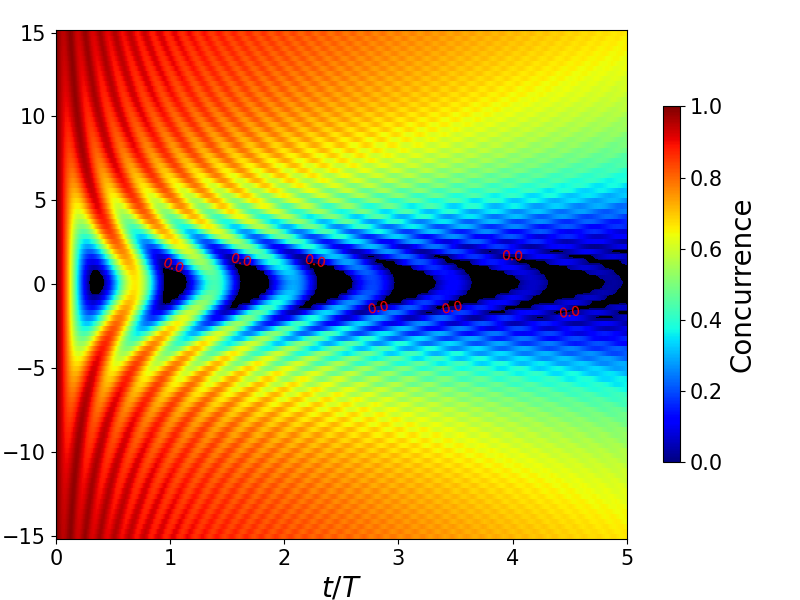
\includegraphics[width=\textwidth]{figuras/ch4/concu/delta/eg0+ge0 k=0.0g x=0.1g J=0.0g gamma=0.25g concu delta dis.png}
        \caption{$\chi=0.1g$}
        \label{fig4:concu detunning x1}
    \end{subfigure}
    \hfill
    \begin{subfigure}{0.49\textwidth}
        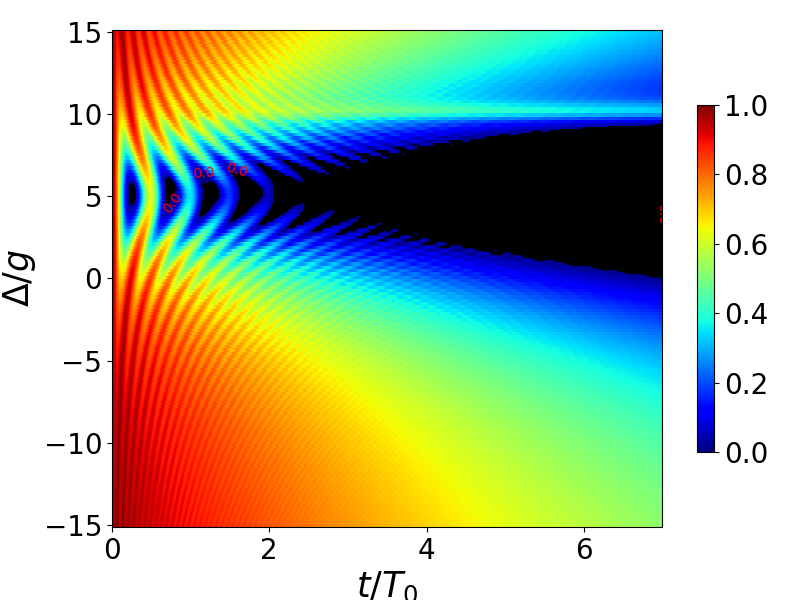
\includegraphics[width=\textwidth]{figuras/ch4/concu/delta/eg0+ge0 k=0.0g x=5.0g J=0.0g gamma=0.25g concu delta dis.png}
        \caption{$\chi=5g$}
        \label{fig4:concu detunning x2}
    \end{subfigure}
    \vfill
    \begin{subfigure}{0.49\textwidth}
        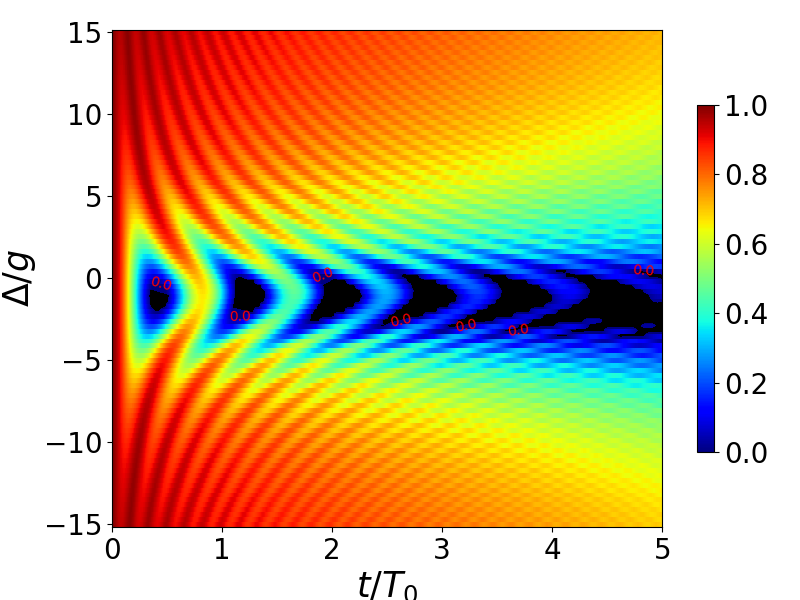
\includegraphics[width=\textwidth]{figuras/ch4/concu/delta/eg0+ge0 k=0.5g x=0.0g J=0.0g gamma=0.25g concu delta dis.png}
        \caption{$k-J=0.5g$}
        \label{fig4:concu detunning k1}
    \end{subfigure}
    \hfill
    \begin{subfigure}{0.49\textwidth}
        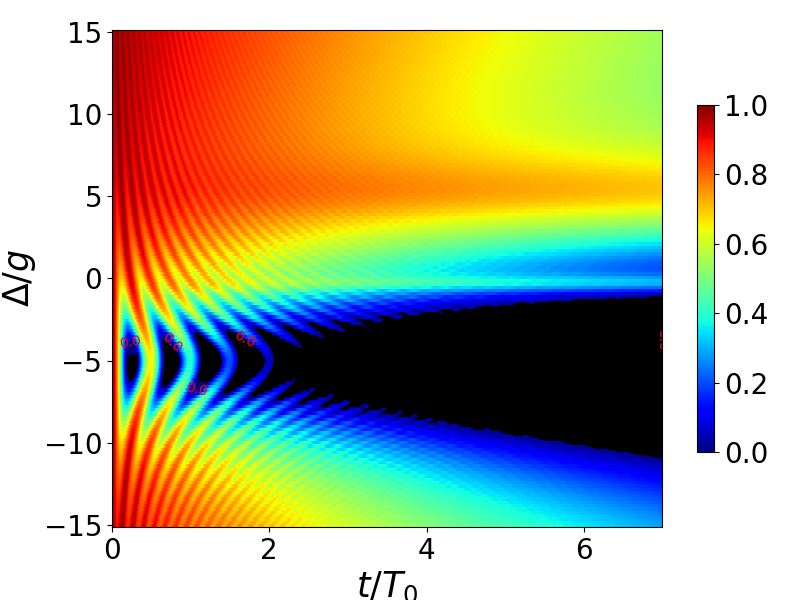
\includegraphics[width=\textwidth]{figuras/ch4/concu/delta/eg0+ge0 k=2.5g x=0.0g J=0.0g gamma=0.25g concu delta dis.png}
        \caption{$k-J=2.5g$}
        \label{fig4:concu detunning k2}
    \end{subfigure}
    \caption{}
    \label{fig4:concu detunning 0 params}
\end{figure}

\subsubsection{\underline{Condicion inicial $\ket{eg1+ge1}$}}
En la figura \ref{fig4:concu detunning 1} se observa la evolución de la concurrencia para la condición inicial $\ket{eg0+ge0}$, cuyo entrelazamiento entre los átomos es máximo. En el eje x es el tiempo, y en el eje y es el detunning $\Delta/g$. En el panel \ref{fig4:concu detunning 0 uni} se observa como oscila la concurrencia, llegando al cero periódicamente. Se ve como al aumentar el detunning, estas oscilaciones son cada vez de menor amplitud, y el entrelazamiento se mantiene. Ademas, la frecuencia de oscilación es cada vez mayor. Al tomar la dinámica disipativa, en el panel \ref{fig4:concu detunning 0 dis}, se observa como las oscilaciones siguen estando, pero ahora su máximo disminuye con el tiempo. Esto es de esperarse, ya que la cavidad deja escapar fotones y el estado del sistema se hace mixto. Un estado mixto ya no es entrelazado, porque no hay coherencias, entonces se observa el deterioro del entrelazamiento a medida que el tiempo avanza. Hay otros dos comportamientos notables. Por un lado, se observa como el máximo del entrelazamiento decae mas lentamente para valores mas altos del detunning, esto se debe a la naturaleza da la dinámica poblacional; al aumentar el detunning, como se vio anteriormente, uno de los efectos principales es que las oscilaciones entre los estados tienen poca amplitud, y en este caso, esto implica que si bien el estado $\ket{gg1}$ tienen amplitudes no nula, principalmente el estado del sistema esta concentrado en el estado inicial, que no sufre decoherencia por perdida de fotones, ya que no tiene fotones en la cavidad. Entonces, mientras mayor el detunning, menor la probabilidad de encontrar al sistema en el estado $\ket{gg1}$, y por lo tanto tiene pocas probabilidades de perder fotones. El otro efecto que es interesante y que aparece con frecuencia en este tipo de sistemas, es la muerte y reanimación súbita del entrelazamiento, que llamaremos SDE (Sudden Death Effect) y SBE (Sudden Birth Effect) por sus siglas en ingles. En el caso disipativo, hay marcadas zonas en negro, estas muestran como el entrelazamiento \textit{muere} durante un tiempo finito y reviven luego. Este efecto es sorprendente, ya que uno espera que las coherencias, responsables en gran medida del entrelazamiento entre átomos, decaigan asintóticamente. 

\begin{figure}[h]
    \centering
    \begin{subfigure}{0.49\textwidth}
        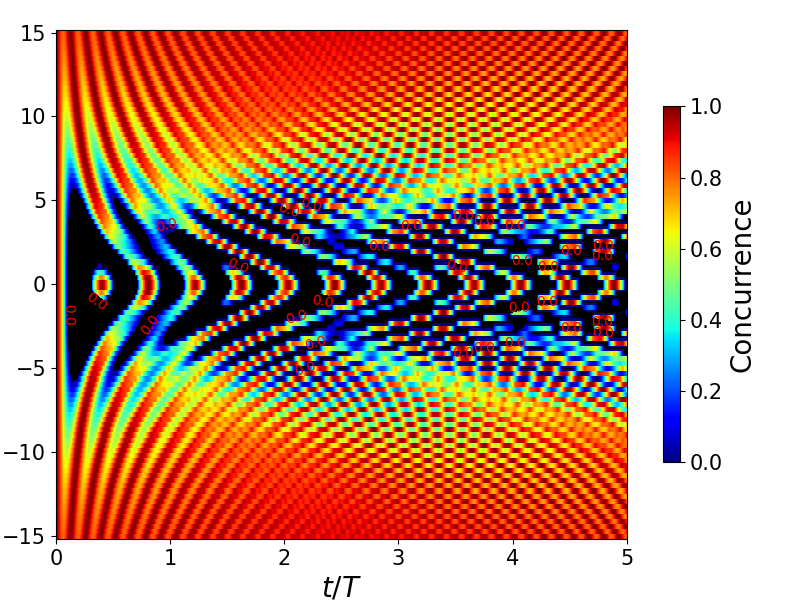
\includegraphics[width=\textwidth]{figuras/ch4/concu/delta/eg1+ge1 k=0.0g x=0.0g J=0.0g gamma=0.25g concu delta uni.png}
        \caption{Dinámica sin perdidas}
        \label{fig4:concu detunning 1 uni}
    \end{subfigure}
    \hfill
    \begin{subfigure}{0.49\textwidth}
        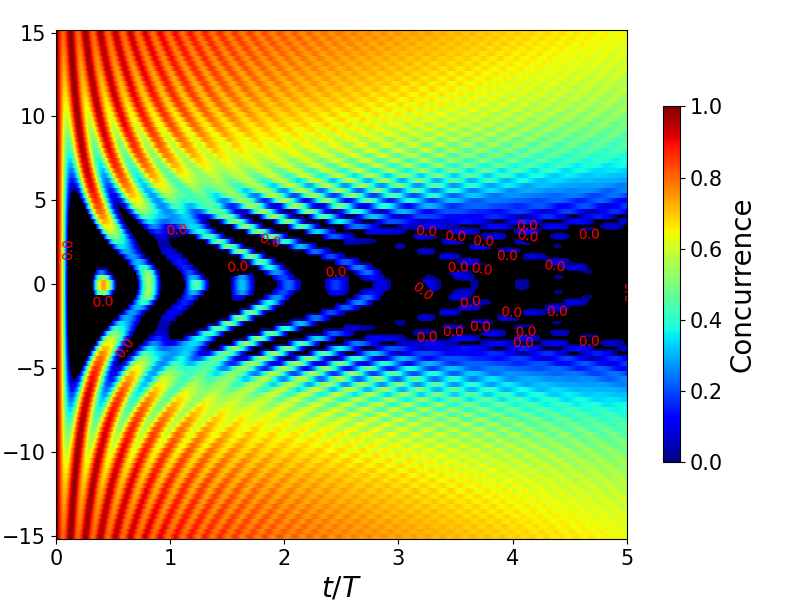
\includegraphics[width=\textwidth]{figuras/ch4/concu/delta/eg1+ge1 k=0.0g x=0.0g J=0.0g gamma=0.25g concu delta dis.png}
        \caption{Dinámica con perdidas}
        \label{fig4:concu detunning 1 dis}
    \end{subfigure}
    \caption{Dinámica de entrelazamiento para el estado inicial $\ket{eg0+ge0}$, en función del detunning, y para $\chi=k-J=0$.}
    \label{fig4:concu detunning 1}
\end{figure}

La pregunta natural que sigue es si cambiar los parametros $\chi$ y $k-J$, cambia la forma de la figura \ref{fig4:concu detunning 0}. Es de esperar que no cambie, ya que el subespacio de $N=1$ se comporta de manera sencilla, y como se concluyo anteriormente, la dependencia en los parametros $\chi$ y $k-J$ parece ser unicamente un desplazamiento de las energias de los autoestados. En la figura \ref{fig4:concu detunning 1} se muestran nuevamente la dinamica de entrelazamiento en funcion del detunning, pero ahora cambiando alguno de los parametros:

\begin{figure}[h]
    \centering
    \begin{subfigure}{0.49\textwidth}
        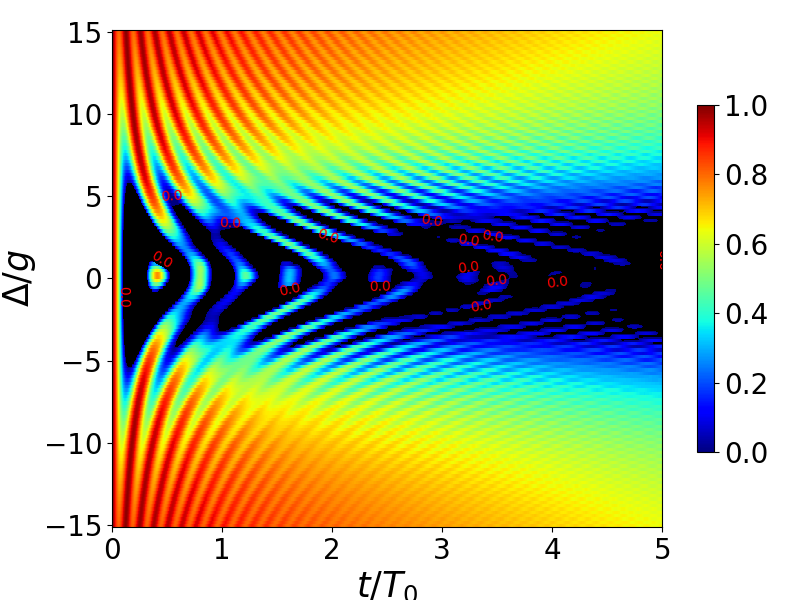
\includegraphics[width=\textwidth]{figuras/ch4/concu/delta/eg1+ge1 k=0.0g x=0.1g J=0.0g gamma=0.25g concu delta dis.png}
        \caption{$\chi=0.1g$}
        \label{fig4:concu detunning 1 x1}
    \end{subfigure}
    \hfill
    \begin{subfigure}{0.49\textwidth}
        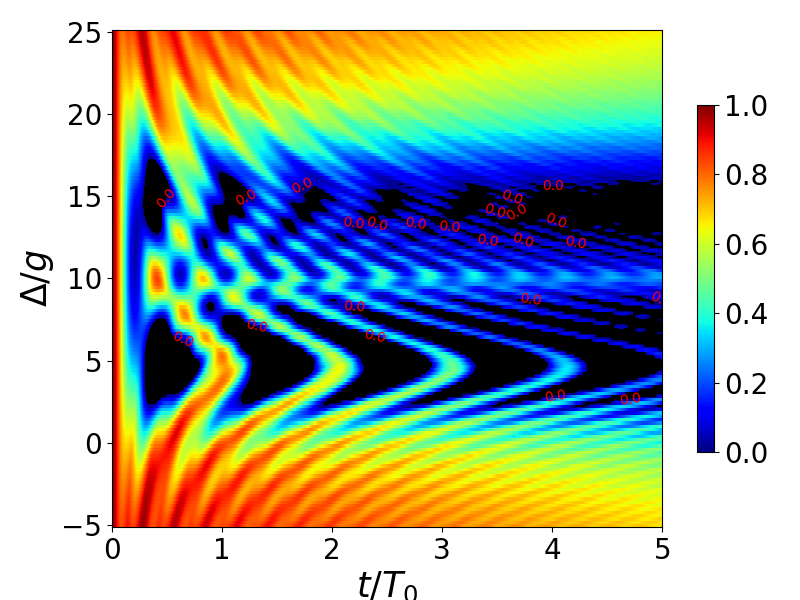
\includegraphics[width=\textwidth]{figuras/ch4/concu/delta/eg1+ge1 k=0.0g x=5.0g J=0.0g gamma=0.25g concu delta dis.png}
        \caption{$\chi=5g$}
        \label{fig4:concu detunning 1 x2}
    \end{subfigure}
    \vfill
    \begin{subfigure}{0.49\textwidth}
        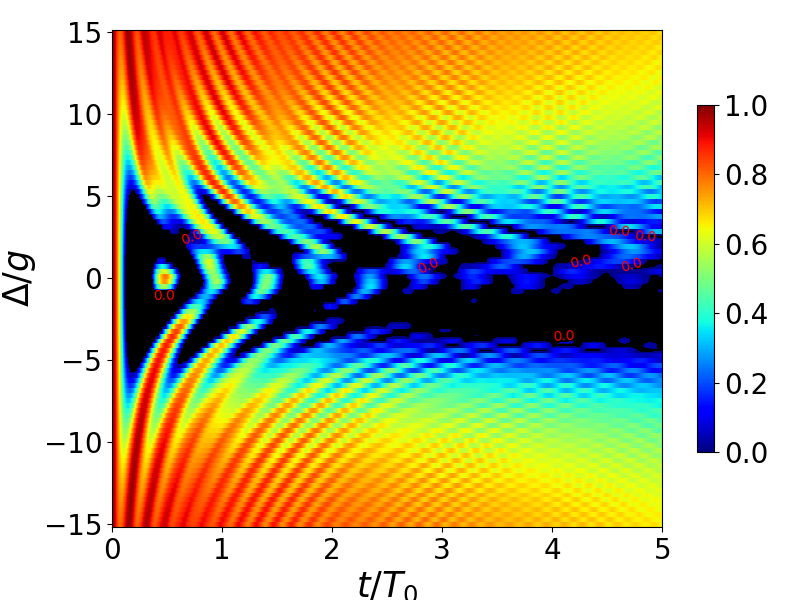
\includegraphics[width=\textwidth]{figuras/ch4/concu/delta/eg1+ge1 k=0.5g x=0.0g J=0.0g gamma=0.25g concu delta dis.png}
        \caption{$k-J=0.5g$}
        \label{fig4:concu detunning 1 k1}
    \end{subfigure}
    \hfill
    \begin{subfigure}{0.49\textwidth}
        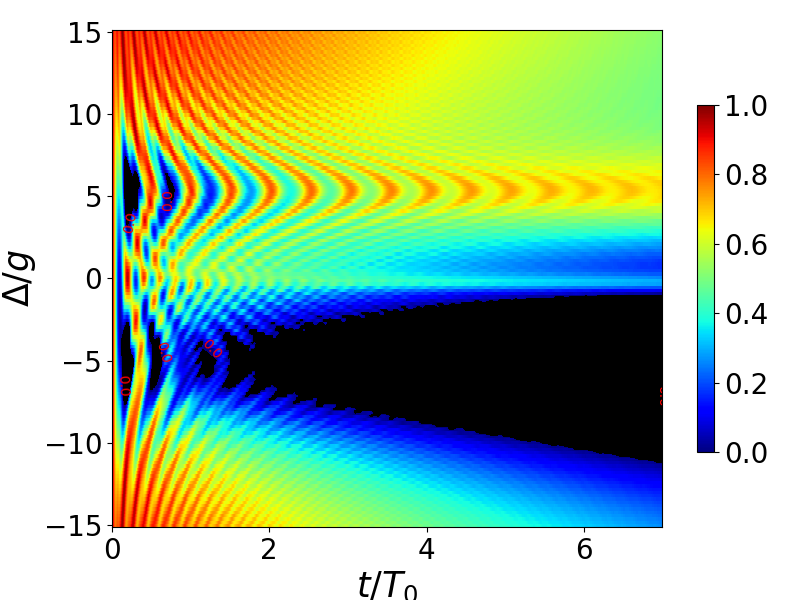
\includegraphics[width=\textwidth]{figuras/ch4/concu/delta/eg1+ge1 k=2.5g x=0.0g J=0.0g gamma=0.25g concu delta dis.png}
        \caption{$k-J=2.5g$}
        \label{fig4:concu detunning 1 k2}
    \end{subfigure}
    \caption{}
    \label{fig4:concu detunning 1 params}
\end{figure}
\subsubsection{\underline{Condicion inicial $\ket{3er0}$}}

\subsection{Dependencia con el medio $\chi$}
\subsubsection{\underline{Condicion inicial $\ket{eg0+ge0}$}}
\begin{figure}[h]
    \centering
    \begin{subfigure}{0.49\textwidth}
        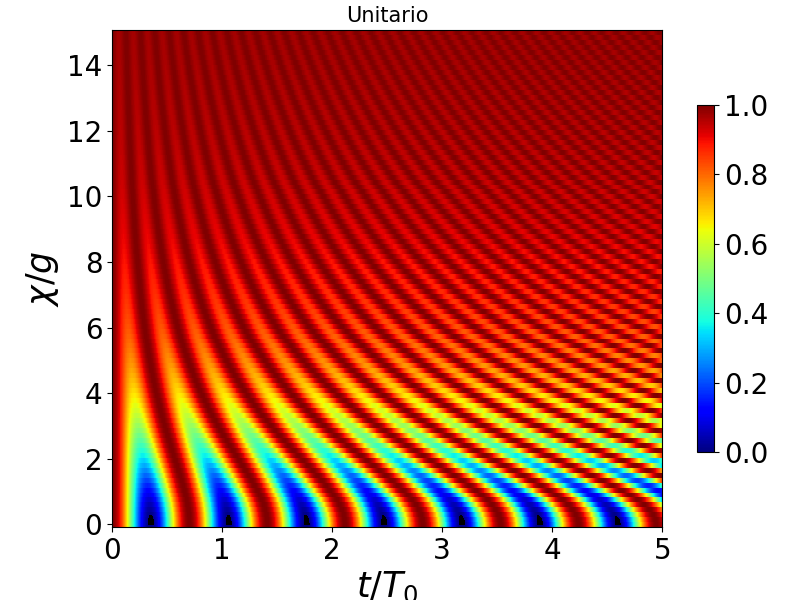
\includegraphics[width=\textwidth]{figuras/ch4/concu/chi/eg0+ge0 d=0.0g k=0.0g J=0.0g gamma=0.25g concu chi uni.png}
        \caption{Dinámica sin perdidas}
        \label{fig4:concu x 0 uni}
    \end{subfigure}
    \hfill
    \begin{subfigure}{0.49\textwidth}
        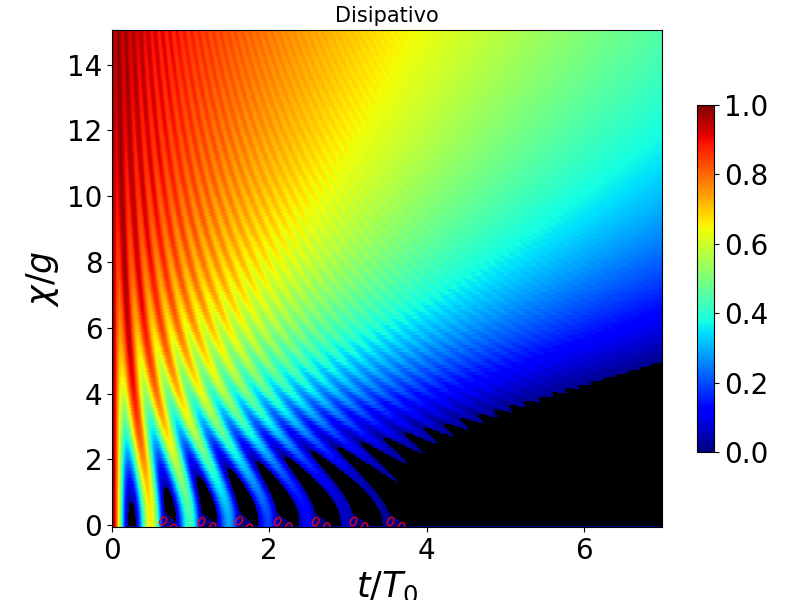
\includegraphics[width=\textwidth]{figuras/ch4/concu/chi/eg0+ge0 d=0.0g k=0.0g J=0.0g gamma=0.25g concu chi dis.png}
        \caption{Dinámica con perdidas}
        \label{fig4:concu x 0 dis}
    \end{subfigure}
    \caption{Dinámica de entrelazamiento para el estado inicial $\ket{eg0+ge0}$, en función del detunning, y para $\chi=k-J=0$.}
    \label{fig4:concu x 0}
\end{figure}
En la figura \ref{fig4:concu x 0} se observa la evolución de la concurrencia para la condición inicial $\ket{eg0+ge0}$, cuyo entrelazamiento entre los átomos es máximo. En el eje x es el tiempo, y en el eje y es el detunning $\Delta/g$. En el panel \ref{fig4:concu detunning 0 uni} se observa como oscila la concurrencia, llegando al cero periódicamente. Se ve como al aumentar el detunning, estas oscilaciones son cada vez de menor amplitud, y el entrelazamiento se mantiene. Ademas, la frecuencia de oscilación es cada vez mayor. Al tomar la dinámica disipativa, en el panel \ref{fig4:concu detunning 0 dis}, se observa como las oscilaciones siguen estando, pero ahora su máximo disminuye con el tiempo. Esto es de esperarse, ya que la cavidad deja escapar fotones y el estado del sistema se hace mixto. Un estado mixto ya no es entrelazado, porque no hay coherencias, entonces se observa el deterioro del entrelazamiento a medida que el tiempo avanza. Hay otros dos comportamientos notables. Por un lado, se observa como el máximo del entrelazamiento decae mas lentamente para valores mas altos del detunning, esto se debe a la naturaleza da la dinámica poblacional; al aumentar el detunning, como se vio anteriormente, uno de los efectos principales es que las oscilaciones entre los estados tienen poca amplitud, y en este caso, esto implica que si bien el estado $\ket{gg1}$ tienen amplitudes no nula, principalmente el estado del sistema esta concentrado en el estado inicial, que no sufre decoherencia por perdida de fotones, ya que no tiene fotones en la cavidad. Entonces, mientras mayor el detunning, menor la probabilidad de encontrar al sistema en el estado $\ket{gg1}$, y por lo tanto tiene pocas probabilidades de perder fotones. El otro efecto que es interesante y que aparece con frecuencia en este tipo de sistemas, es la muerte y reanimación súbita del entrelazamiento, que llamaremos SDE (Sudden Death Effect) y SBE (Sudden Birth Effect) por sus siglas en ingles. En el caso disipativo, hay marcadas zonas en negro, estas muestran como el entrelazamiento \textit{muere} durante un tiempo finito y reviven luego. Este efecto es sorprendente, ya que uno espera que las coherencias, responsables en gran medida del entrelazamiento entre átomos, decaigan asintóticamente. 

La pregunta natural que sigue es si cambiar los parametros $\chi$ y $k-J$, cambia la forma de la figura \ref{fig4:concu detunning 0}. Es de esperar que no cambie, ya que el subespacio de $N=1$ se comporta de manera sencilla, y como se concluyo anteriormente, la dependencia en los parametros $\chi$ y $k-J$ parece ser unicamente un desplazamiento de las energias de los autoestados. En la figura \ref{fig4:concu detunning 1} se muestran nuevamente la dinamica de entrelazamiento en funcion del detunning, pero ahora cambiando alguno de los parametros:

\begin{figure}[h]
    \centering
    \begin{subfigure}{0.49\textwidth}
        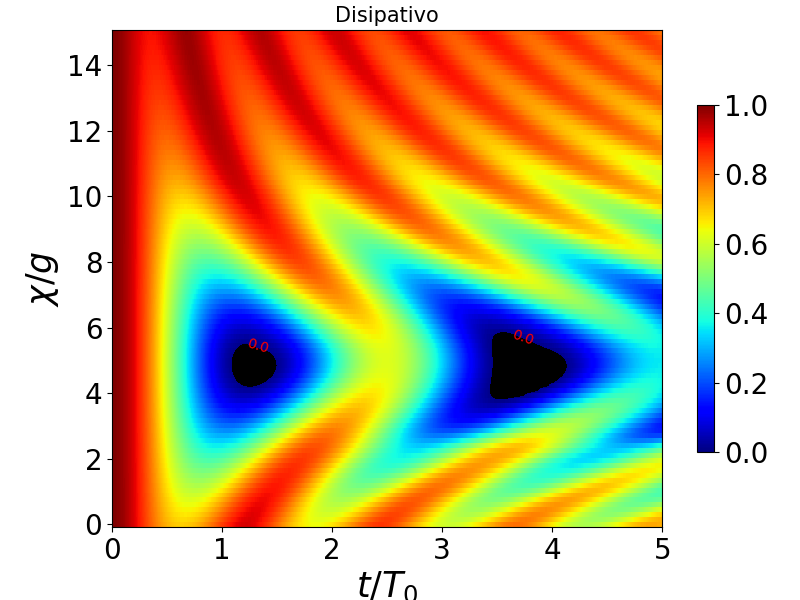
\includegraphics[width=\textwidth]{figuras/ch4/concu/chi/eg0+ge0 d=5.0g k=0.0g J=0.0g gamma=0.25g concu chi dis.png}
        \caption{$\chi=0.1g$}
        \label{fig4:concu x d1}
    \end{subfigure}
    \hfill
    \begin{subfigure}{0.49\textwidth}
        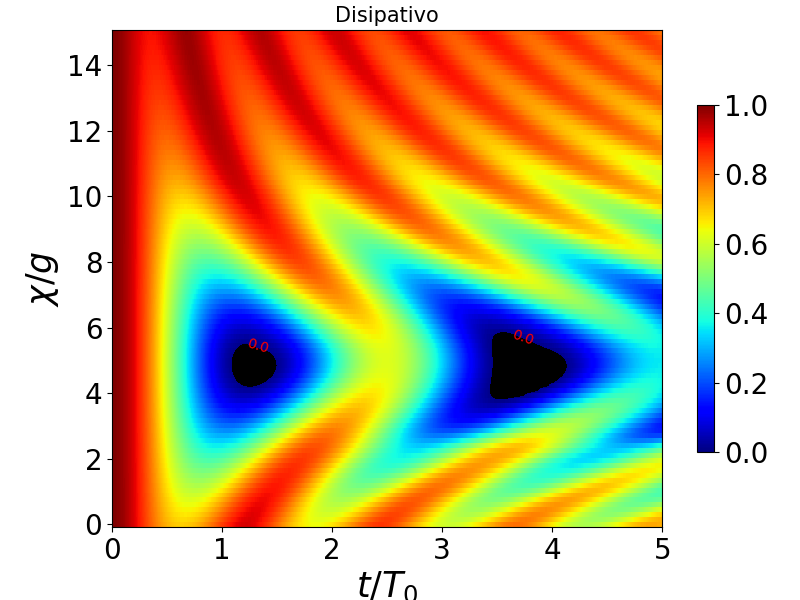
\includegraphics[width=\textwidth]{figuras/ch4/concu/chi/eg0+ge0 d=5.0g k=0.0g J=0.0g gamma=0.25g concu chi dis.png}
        \caption{$\chi=5g$}
        \label{fig4:concu x d2}
    \end{subfigure}
    \vfill
    \begin{subfigure}{0.49\textwidth}
        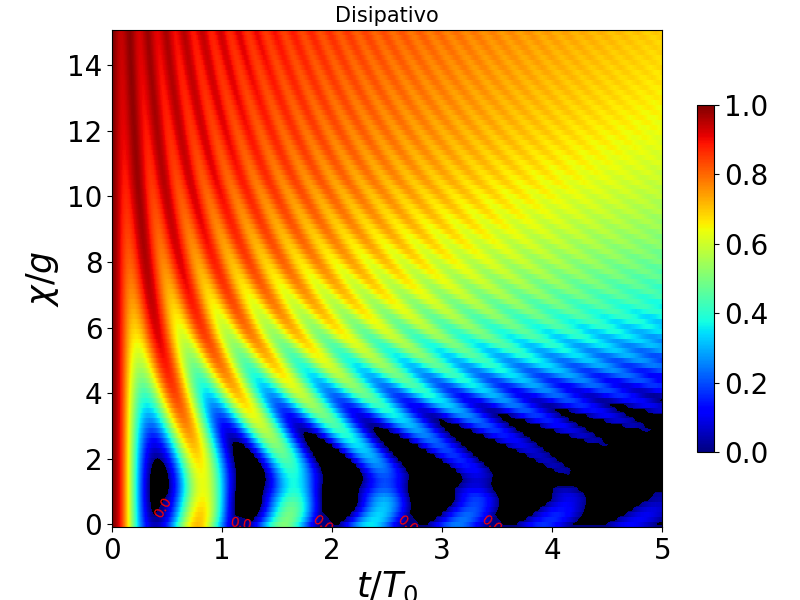
\includegraphics[width=\textwidth]{figuras/ch4/concu/chi/eg0+ge0 d=0.0g k=0.5g J=0.0g gamma=0.25g concu chi dis.png}
        \caption{$k-J=0.5g$}
        \label{fig4:concu x k1}
    \end{subfigure}
    \hfill
    \begin{subfigure}{0.49\textwidth}
        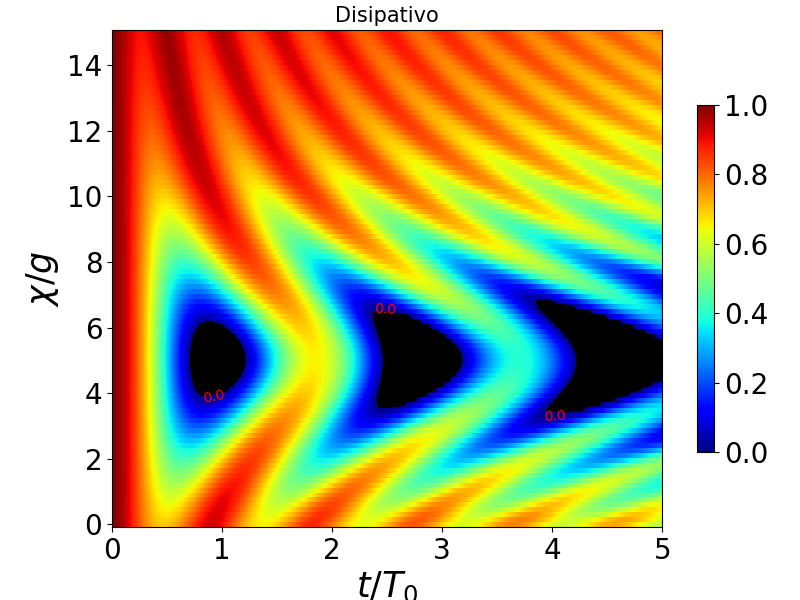
\includegraphics[width=\textwidth]{figuras/ch4/concu/chi/eg0+ge0 d=0.0g k=2.5g J=0.0g gamma=0.25g concu chi dis.png}
        \caption{$k-J=2.5g$}
        \label{fig4:concu x k2}
    \end{subfigure}
    \caption{}
    \label{fig4:concu x params}
\end{figure}
\subsubsection{\underline{Condicion inicial $\ket{eg1+ge1}$}}
\begin{figure}[h]
    \centering
    \begin{subfigure}{0.49\textwidth}
        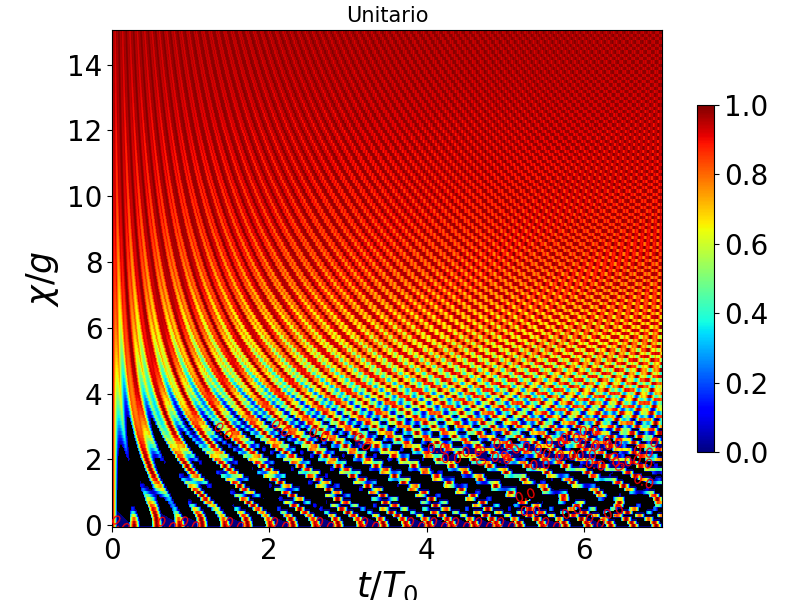
\includegraphics[width=\textwidth]{figuras/ch4/concu/chi/eg1+ge1 d=0.0g k=0.0g J=0.0g gamma=0.25g concu chi uni.png}
        \caption{Dinámica sin perdidas}
        \label{fig4:concu x 1 uni}
    \end{subfigure}
    \hfill
    \begin{subfigure}{0.49\textwidth}
        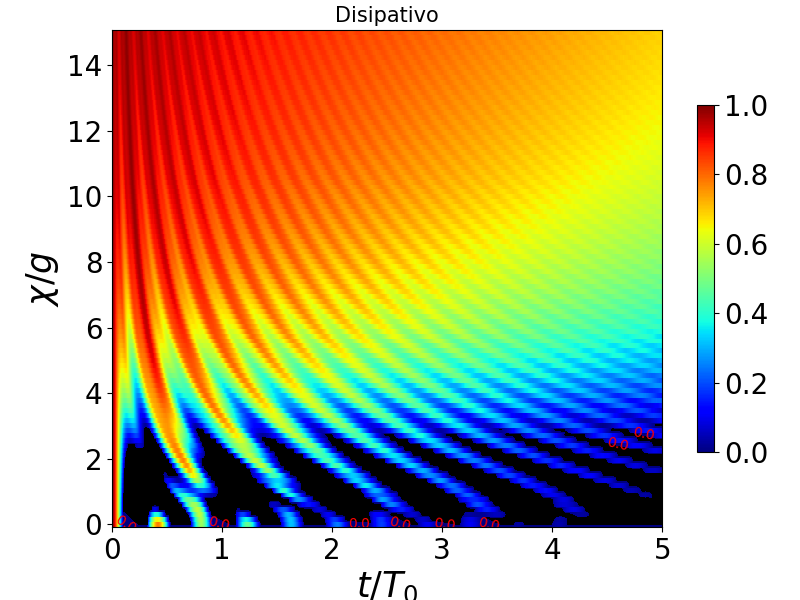
\includegraphics[width=\textwidth]{figuras/ch4/concu/chi/eg1+ge1 d=0.0g k=0.0g J=0.0g gamma=0.25g concu chi dis.png}
        \caption{Dinámica con perdidas}
        \label{fig4:concu x 1 dis}
    \end{subfigure}
    \caption{Dinámica de entrelazamiento para el estado inicial $\ket{eg0+ge0}$, en función del detunning, y para $\chi=k-J=0$.}
    \label{fig4:concu x 1}
\end{figure}
En la figura \ref{fig4:concu detunning 0} se observa la evolución de la concurrencia para la condición inicial $\ket{eg0+ge0}$, cuyo entrelazamiento entre los átomos es máximo. En el eje x es el tiempo, y en el eje y es el detunning $\Delta/g$. En el panel \ref{fig4:concu detunning 0 uni} se observa como oscila la concurrencia, llegando al cero periódicamente. Se ve como al aumentar el detunning, estas oscilaciones son cada vez de menor amplitud, y el entrelazamiento se mantiene. Ademas, la frecuencia de oscilación es cada vez mayor. Al tomar la dinámica disipativa, en el panel \ref{fig4:concu detunning 0 dis}, se observa como las oscilaciones siguen estando, pero ahora su máximo disminuye con el tiempo. Esto es de esperarse, ya que la cavidad deja escapar fotones y el estado del sistema se hace mixto. Un estado mixto ya no es entrelazado, porque no hay coherencias, entonces se observa el deterioro del entrelazamiento a medida que el tiempo avanza. Hay otros dos comportamientos notables. Por un lado, se observa como el máximo del entrelazamiento decae mas lentamente para valores mas altos del detunning, esto se debe a la naturaleza da la dinámica poblacional; al aumentar el detunning, como se vio anteriormente, uno de los efectos principales es que las oscilaciones entre los estados tienen poca amplitud, y en este caso, esto implica que si bien el estado $\ket{gg1}$ tienen amplitudes no nula, principalmente el estado del sistema esta concentrado en el estado inicial, que no sufre decoherencia por perdida de fotones, ya que no tiene fotones en la cavidad. Entonces, mientras mayor el detunning, menor la probabilidad de encontrar al sistema en el estado $\ket{gg1}$, y por lo tanto tiene pocas probabilidades de perder fotones. El otro efecto que es interesante y que aparece con frecuencia en este tipo de sistemas, es la muerte y reanimación súbita del entrelazamiento, que llamaremos SDE (Sudden Death Effect) y SBE (Sudden Birth Effect) por sus siglas en ingles. En el caso disipativo, hay marcadas zonas en negro, estas muestran como el entrelazamiento \textit{muere} durante un tiempo finito y reviven luego. Este efecto es sorprendente, ya que uno espera que las coherencias, responsables en gran medida del entrelazamiento entre átomos, decaigan asintóticamente. 

La pregunta natural que sigue es si cambiar los parametros $\chi$ y $k-J$, cambia la forma de la figura \ref{fig4:concu detunning 0}. Es de esperar que no cambie, ya que el subespacio de $N=1$ se comporta de manera sencilla, y como se concluyo anteriormente, la dependencia en los parametros $\chi$ y $k-J$ parece ser unicamente un desplazamiento de las energias de los autoestados. En la figura \ref{fig4:concu detunning 1} se muestran nuevamente la dinamica de entrelazamiento en funcion del detunning, pero ahora cambiando alguno de los parametros:

\begin{figure}[h]
    \centering
    \begin{subfigure}{0.49\textwidth}
        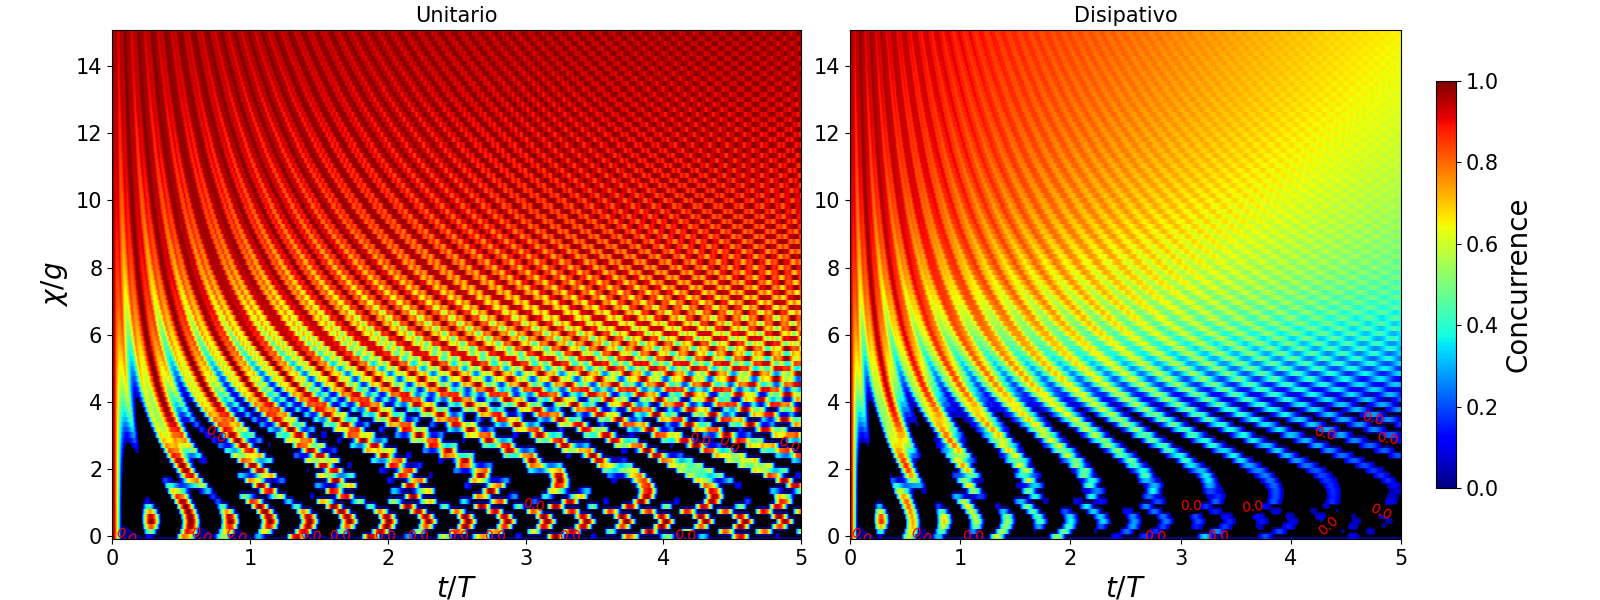
\includegraphics[width=\textwidth]{figuras/ch4/concu/chi/eg1+ge1 d=1.0g k=0.0g J=0.0g gamma=0.1g concu chi.png}
        \caption{$\chi=0.1g$}
        \label{fig4:concu x 1 k1}
    \end{subfigure}
    \hfill
    \begin{subfigure}{0.49\textwidth}
        \includegraphics[width=\textwidth]{figuras/ch4/concu/chi/eg1+ge1 d=5.0g k=0.0g J=0.0g gamma=0.25g concu chi uni.png}
        \caption{$\chi=5g$}
        \label{fig4:concu x 1 k2}
    \end{subfigure}
    \vfill
    \begin{subfigure}{0.49\textwidth}
        \includegraphics[width=\textwidth]{figuras/ch4/concu/chi/eg1+ge1 d=0.0g k=0.5g J=0.0g gamma=0.25g concu chi dis.png}
        \caption{$k-J=0.5g$}
        \label{fig4:concu x 1 d1}
    \end{subfigure}
    \hfill
    \begin{subfigure}{0.49\textwidth}
        \includegraphics[width=\textwidth]{figuras/ch4/concu/chi/eg1+ge1 d=0.0g k=2.5g J=0.0g gamma=0.25g concu chi dis.png}
        \caption{$k-J=2.5g$}
        \label{fig4:concu x 1 d2}
    \end{subfigure}
    \caption{}
    \label{}
\end{figure}
\subsubsection{\underline{Condicion inicial $\ket{3er0}$}}


\subsection{Dependencia con la interaccion $k-J$}
\subsubsection{\underline{Condicion inicial $\ket{eg0+ge0}$}}
\begin{figure}[h]
    \centering
    \begin{subfigure}{0.49\textwidth}
        \includegraphics[width=\textwidth]{figuras/ch4/concu/k/eg0+ge0 d=0.0g x=0.0g J=0.0g gamma=0.25g concu k uni.png}
        \caption{Dinámica sin perdidas}
        \label{fig4:concu k 0 uni}
    \end{subfigure}
    \hfill
    \begin{subfigure}{0.49\textwidth}
        \includegraphics[width=\textwidth]{figuras/ch4/concu/k/eg0+ge0 d=0.0g x=0.0g J=0.0g gamma=0.25g concu k dis.png}
        \caption{Dinámica con perdidas}
        \label{fig4:concu k 0 dis}
    \end{subfigure}
    \caption{Dinámica de entrelazamiento para el estado inicial $\ket{eg0+ge0}$, en función del detunning, y para $\chi=k-J=0$.}
    \label{fig4:concu k 0}
\end{figure}
En la figura \ref{fig4:concu k 0} se observa la evolución de la concurrencia para la condición inicial $\ket{eg0+ge0}$, cuyo entrelazamiento entre los átomos es máximo. En el eje x es el tiempo, y en el eje y es el detunning $\Delta/g$. En el panel \ref{fig4:concu detunning 0 uni} se observa como oscila la concurrencia, llegando al cero periódicamente. Se ve como al aumentar el detunning, estas oscilaciones son cada vez de menor amplitud, y el entrelazamiento se mantiene. Ademas, la frecuencia de oscilación es cada vez mayor. Al tomar la dinámica disipativa, en el panel \ref{fig4:concu detunning 0 dis}, se observa como las oscilaciones siguen estando, pero ahora su máximo disminuye con el tiempo. Esto es de esperarse, ya que la cavidad deja escapar fotones y el estado del sistema se hace mixto. Un estado mixto ya no es entrelazado, porque no hay coherencias, entonces se observa el deterioro del entrelazamiento a medida que el tiempo avanza. Hay otros dos comportamientos notables. Por un lado, se observa como el máximo del entrelazamiento decae mas lentamente para valores mas altos del detunning, esto se debe a la naturaleza da la dinámica poblacional; al aumentar el detunning, como se vio anteriormente, uno de los efectos principales es que las oscilaciones entre los estados tienen poca amplitud, y en este caso, esto implica que si bien el estado $\ket{gg1}$ tienen amplitudes no nula, principalmente el estado del sistema esta concentrado en el estado inicial, que no sufre decoherencia por perdida de fotones, ya que no tiene fotones en la cavidad. Entonces, mientras mayor el detunning, menor la probabilidad de encontrar al sistema en el estado $\ket{gg1}$, y por lo tanto tiene pocas probabilidades de perder fotones. El otro efecto que es interesante y que aparece con frecuencia en este tipo de sistemas, es la muerte y reanimación súbita del entrelazamiento, que llamaremos SDE (Sudden Death Effect) y SBE (Sudden Birth Effect) por sus siglas en ingles. En el caso disipativo, hay marcadas zonas en negro, estas muestran como el entrelazamiento \textit{muere} durante un tiempo finito y reviven luego. Este efecto es sorprendente, ya que uno espera que las coherencias, responsables en gran medida del entrelazamiento entre átomos, decaigan asintóticamente. 

La pregunta natural que sigue es si cambiar los parametros $\chi$ y $k-J$, cambia la forma de la figura \ref{fig4:concu detunning 0}. Es de esperar que no cambie, ya que el subespacio de $N=1$ se comporta de manera sencilla, y como se concluyo anteriormente, la dependencia en los parametros $\chi$ y $k-J$ parece ser unicamente un desplazamiento de las energias de los autoestados. En la figura \ref{fig4:concu detunning 1} se muestran nuevamente la dinamica de entrelazamiento en funcion del detunning, pero ahora cambiando alguno de los parametros:

\begin{figure}[h]
    \centering
    \begin{subfigure}{0.49\textwidth}
        \includegraphics[width=\textwidth]{figuras/ch4/concu/k/eg0+ge0 d=5.0g x=0.0g J=0.0g gamma=0.25g concu k dis.png}
        \caption{$\chi=0.1g$}
        \label{fig4:concu k x1}
    \end{subfigure}
    \hfill
    \begin{subfigure}{0.49\textwidth}
        \includegraphics[width=\textwidth]{figuras/ch4/concu/k/eg0+ge0 d=5.0g x=0.0g J=0.0g gamma=0.25g concu k dis.png}
        \caption{$\chi=5g$}
        \label{fig4:concu k x2}
    \end{subfigure}
    \vfill
    \begin{subfigure}{0.49\textwidth}
        \includegraphics[width=\textwidth]{figuras/ch4/concu/k/eg0+ge0 d=0.0g x=0.5g J=0.0g gamma=0.25g concu k dis.png}
        \caption{$k-J=0.5g$}
        \label{fig4:concu k d1}
    \end{subfigure}
    \hfill
    \begin{subfigure}{0.49\textwidth}
        \includegraphics[width=\textwidth]{figuras/ch4/concu/k/eg0+ge0 d=0.0g x=5.0g J=0.0g gamma=0.25g concu k dis.png}
        \caption{$k-J=2.5g$}
        \label{fig4:concu k d2}
    \end{subfigure}
    \caption{}
    \label{}
\end{figure}
\subsubsection{\underline{Condicion inicial $\ket{eg1+ge1}$}}
\begin{figure}[h]
    \centering
    \begin{subfigure}{0.49\textwidth}
        \includegraphics[width=\textwidth]{figuras/ch4/concu/k/eg1+ge1 d=0.0g x=0.0g J=0.0g gamma=0.25g concu k uni.png}
        \caption{Dinámica sin perdidas}
        \label{fig4:concu k 1 uni}
    \end{subfigure}
    \hfill
    \begin{subfigure}{0.49\textwidth}
        \includegraphics[width=\textwidth]{figuras/ch4/concu/k/eg1+ge1 d=0.0g x=0.0g J=0.0g gamma=0.25g concu k dis.png}
        \caption{Dinámica con perdidas}
        \label{fig4:concu k 1 dis}
    \end{subfigure}
    \caption{Dinámica de entrelazamiento para el estado inicial $\ket{eg0+ge0}$, en función del detunning, y para $\chi=k-J=0$.}
    \label{fig4:concu k 1}
\end{figure}
En la figura \ref{fig4:concu k 1} se observa la evolución de la concurrencia para la condición inicial $\ket{eg0+ge0}$, cuyo entrelazamiento entre los átomos es máximo. En el eje x es el tiempo, y en el eje y es el detunning $\Delta/g$. En el panel \ref{fig4:concu detunning 0 uni} se observa como oscila la concurrencia, llegando al cero periódicamente. Se ve como al aumentar el detunning, estas oscilaciones son cada vez de menor amplitud, y el entrelazamiento se mantiene. Ademas, la frecuencia de oscilación es cada vez mayor. Al tomar la dinámica disipativa, en el panel \ref{fig4:concu detunning 0 dis}, se observa como las oscilaciones siguen estando, pero ahora su máximo disminuye con el tiempo. Esto es de esperarse, ya que la cavidad deja escapar fotones y el estado del sistema se hace mixto. Un estado mixto ya no es entrelazado, porque no hay coherencias, entonces se observa el deterioro del entrelazamiento a medida que el tiempo avanza. Hay otros dos comportamientos notables. Por un lado, se observa como el máximo del entrelazamiento decae mas lentamente para valores mas altos del detunning, esto se debe a la naturaleza da la dinámica poblacional; al aumentar el detunning, como se vio anteriormente, uno de los efectos principales es que las oscilaciones entre los estados tienen poca amplitud, y en este caso, esto implica que si bien el estado $\ket{gg1}$ tienen amplitudes no nula, principalmente el estado del sistema esta concentrado en el estado inicial, que no sufre decoherencia por perdida de fotones, ya que no tiene fotones en la cavidad. Entonces, mientras mayor el detunning, menor la probabilidad de encontrar al sistema en el estado $\ket{gg1}$, y por lo tanto tiene pocas probabilidades de perder fotones. El otro efecto que es interesante y que aparece con frecuencia en este tipo de sistemas, es la muerte y reanimación súbita del entrelazamiento, que llamaremos SDE (Sudden Death Effect) y SBE (Sudden Birth Effect) por sus siglas en ingles. En el caso disipativo, hay marcadas zonas en negro, estas muestran como el entrelazamiento \textit{muere} durante un tiempo finito y reviven luego. Este efecto es sorprendente, ya que uno espera que las coherencias, responsables en gran medida del entrelazamiento entre átomos, decaigan asintóticamente. 

La pregunta natural que sigue es si cambiar los parametros $\chi$ y $k-J$, cambia la forma de la figura \ref{fig4:concu detunning 0}. Es de esperar que no cambie, ya que el subespacio de $N=1$ se comporta de manera sencilla, y como se concluyo anteriormente, la dependencia en los parametros $\chi$ y $k-J$ parece ser unicamente un desplazamiento de las energias de los autoestados. En la figura \ref{fig4:concu detunning 1} se muestran nuevamente la dinamica de entrelazamiento en funcion del detunning, pero ahora cambiando alguno de los parametros:

\begin{figure}[h]
    \centering
    \begin{subfigure}{0.49\textwidth}
        \includegraphics[width=\textwidth]{figuras/ch4/concu/k/eg1+ge1 d=5.0g x=0.0g J=0.0g gamma=0.25g concu k dis.png}
        \caption{$\chi=0.1g$}
        \label{fig4:concu k 1 x1}
    \end{subfigure}
    \hfill
    \begin{subfigure}{0.49\textwidth}
        \includegraphics[width=\textwidth]{figuras/ch4/concu/k/eg1+ge1 d=5.0g x=0.0g J=0.0g gamma=0.25g concu k dis.png}
        \caption{$\chi=5g$}
        \label{fig4:concu k 1 x2}
    \end{subfigure}
    \vfill
    \begin{subfigure}{0.49\textwidth}
        \includegraphics[width=\textwidth]{figuras/ch4/concu/k/eg1+ge1 d=0.0g x=0.5g J=0.0g gamma=0.25g concu k dis.png}
        \caption{$k-J=0.5g$}
        \label{fig4:concu k 1 d1}
    \end{subfigure}
    \hfill
    \begin{subfigure}{0.49\textwidth}
        \includegraphics[width=\textwidth]{figuras/ch4/concu/k/eg1+ge1 d=0.0g x=5.0g J=0.0g gamma=0.25g concu k dis.png}
        \caption{$k-J=2.5g$}
        \label{fig4:concu k 1 d2}
    \end{subfigure}
    \caption{}
    \label{fig4:concu k 1}
\end{figure}
\subsubsection{\underline{Condicion inicial $\ket{3er0}$}}


\subsection{Acoplamiento Buck-Sukumar}
Para seguir, se considera el efecto del acoplamiento no lineal entre la cavidad y los atomos que se considero al resolver el problema. Esta contribucion aparece en los elementos no diagonales del Hamiltoniano, e influye unicamente en la dinamica de estados con $N\geq2$, ya que si en la cavidad hay solo una excitacion, entonces $\sqrt{n_{fot}}=1$ y es lo mismo que el acoplamiento lineal. Brevemente se observa entonces las consecuencias de este acoplemiento no lineal sobre el entrelazamiento con las condiciones iniciales de $N=2$.
\subsubsection{$\ket{eg0+ge0}$}
\subsubsection{$\ket{eg1+ge1}$}
\subsubsection{$\ket{3er0}$}

\subsection{Conclusiones del capitulo 4}

\subsection{comentarios para borrar}

eg0+ge0 en un mismo grafico
1. k=J=x=0 
2. k=0.1g, J=0, x=0
3. k=5g, J=0, x=0
eg1+ge1 en un mismo grafico
1. k=J=x=0 
2. k=0.1g, J=0, x=0
3. k=5g, J=0, x=0
ee0+gg2 en un mismo grafico
1. k=J=x=0 
2. k=0.1g, J=0, x=0
3. k=5g, J=0, x=0
GRAFICOS DE ENTRELAZAMIENTO PARA DIFERENTES PARAMETROS. PLOTS CON COLORES DEL PAPER ESE. SDE. 

	\chapter{Fase geometrica en JCM generalizado}
\label{ch:fgdoble}

%CAMBIAR ESTO PARA PERSONALIZARLO A MI GUSTO
\pagestyle{fancy}
\fancyhf{}
\fancyhead[LE]{\nouppercase{\rightmark\hfill}}
\fancyhead[RO]{\nouppercase{\leftmark\hfill}}
\fancyfoot[LE,RO]{\hfill\thepage\hfill}

%   Apendices varios
    \appendix
    \chapter{Derivacion de las ecuaciones maestras}
\label{ap_ecsmaestras}

%CAMBIAR ESTO PARA PERSONALIZARLO A MI GUSTO
\pagestyle{fancy}
\fancyhf{}
\fancyhead[LE]{\nouppercase{\rightmark\hfill}}
\fancyhead[RO]{\nouppercase{\leftmark\hfill}}
\fancyfoot[LE,RO]{\hfill\thepage\hfill}

En este apendice se desarrolla la derivacion d
e la ecuacion de Lindblad, que es la ecuacion maestra que determina la evolucion temporal de una matriz densidad $\rho$, que esta en contacto con un entorno del cual no se conoce la dinamica. La dinamica en conjunto esta regida por un Hamiltoniano que formalmente puede escribirse como
\begin{equation}
    H=H_S+H_B+H_{int}
\end{equation}
donde los subindices se refieren a diferentes partes del problema. En primer lugar S se refiere al sitema de estudio, del cual se quiere encontrar la evolucion temporal, y esta en contacto con un entorno B, entonces $H_B$ es el Hamiltoniano que rige la dinamica del entorno que en principio no conocemos. Finalmente, tenemos la interaccion entre las dos partes, dada por el hamiltoniano de interaccion $H_{int}$.
El conjunto completo se puede pensar como un sistema cerrado, y por lo tanto su evolucion temporal esta formalmente dada por la ecuacion de Schr\"odinger, y su correspondiente operador de evolucion $U(t)$ es
\begin{equation}
    U(t)=\mathcal{T}\exp\left( -i\int_{0}^{t}dt'H(t') \right)
\end{equation}
donde $\mathcal{T}$ indica la prescripcion de ordenamiento temporal, y $U(0)=\mathbb{1}$. Si se representa el estado del sistema total con un operador densidad $\rho_{tot}=\ketbra{\psi(t)}{\psi(t)}$, entonces al aplicar la ecuacion de Schr\"odinger de ambos lados se obtiene que 

\begin{equation}
    \dot\rho_{tot}(t)=-\frac{i}{\hbar}[H(t),\rho_{tot}(t)]
\end{equation}
que es la ecuacion de Louiville-Von Neumann, que describe la trayectoria en el espacio de Hilbert del operador densidad del sistema total cerrado.

Va a ser util trabajar en el \textit{picture} de interaccion, en donde reescribimos el Hamiltoniano separandolo en dos partes
\begin{equation}
    H(t)=H_0+\hat H_I(t)
\end{equation}
la manera de seprar el sistema va a variar de problema a problema, pero en general se tiene que $H_0$ es simplemente la energia de las dos partes del sistema si despreciamos la interaccion entre ellos, y que asumimos es intependiente del tiempo; y luego tenemos $\hat H_I(t)$ que es el Hamiltoniano que describe las interacciones entre los sistemas. Como siempre, notamos $U(t,t_0)$ al operador de evolucion temporal, y el valor de expectacion de un observable $A(t)$ en la representacion de Schroedinger
\begin{equation}
    \langle A(t) \rangle = \tr \{ A(t)U(t,t_0) \rho(t_0)U^\dagger(t,t_0) \}
    \label{ecA1:valor de expectacion}
\end{equation}

Ahora se introducen los operadores unitarios

\begin{equation}
    U_0(t,t_0)\equiv\exp [ -i H_0(t-t_0)]
\end{equation}

con $U_I(t,t_0)\equiv U_0^\dagger(t,t_0)U(t,t_0)$. Entonces el valor de expectacion \ref{eqA1:valor de expectacion} tambien puede escribirse como
\begin{equation}
    \begin{aligned}
    \langle A(t) \rangle &= \tr \{ U_0^\dagger(t,t_0)A(t)U_0(t,t_0)U_I(t,t_0) \rho(t_0)U_I^\dagger(t,t_0) \} \\
    & \equiv \tr \{A_I(t)\rho_I(t) \}
    \end{aligned}
    \label{ecA1:valor de expectacion interaccion}
\end{equation}
donde introducimos al poerador en el \textit{picture} de interaccion, y enontces la matriz densidad evoluciona en esta representacion segundo
\begin{equation}
    \rho_I(t)=U_I(t,t_0)\rho(t_0)U^\dagger_I(t,t_0)
\end{equation}
De esto lo que se debe recordar es que el Hamiltoniano en la repserentacion de interaccion, y la ecuacion de von Neumann se escriben como
\begin{equation}
    H_I(t)=U_0^\dagger(t,t_0)\hat H_I(t)U_0(t,t_0)
\end{equation}
Y
\begin{equation}
    \frac{d}{dt}\rho_I(t)=-i[H_I(t),\rho_I(t)]
\end{equation}
Si integramos esta ecuacion obtenemos la solucion formal
\begin{equation}
    \rho_I(t)=\rho_I(t_0)-i\int_{t_0}^{t}
\end{equation}

% Si ahora se considera que el sistema esta abierto, es decir, que el sistema de interes S esta en contacto con otro sistema cuentoco B que llamamos entorno, entonces el sistema total S+B se puede describir usando lo que escribimos anteriormente. Pero si nos concentramos en la dinamica de el subsistema S, entonces este va a cambiar por la influencia de B, y en general no va a seguir una dinamica Hamiltoniana.
% Llamemos $\mathcal{H_S}$ el espacio de Hilbert del sistema, y $\mathcal{H_B}$ al del entorno. El espacio total del sistema S+B es el producto tensorial $\mathcal{H}=\mathcal{H_S}\otimes\mathcal{H_B}$, y el Hamiltoniano total se puede tomar de la forma
% \begin{equation}
%     H(t)=H_S\otimes I_B +I_S\otimes H_B + \hat H_I(t)
% \end{equation}
% Todos los observables que solo actuan sobre el subespacio S pueden escribirse como $A\otimes I_B$, y si el sistema total se puede describir segun el operador densidad $\rho$, etnonces los valores de expectacion de todos los observables que actuan sobre S estan determinados por
% \begin{equation}
%     \langle A \rangle = \tr_S\{A\rho_S\}
% \end{equation}
% donde 
% \begin{equation}
%     \rho_S=\tr_B \rho
% \end{equation}
% es la matriz densidad reducida del sistema abierto S, y la notacion $\tr_A$ denota la traza parcial sobre los grados de libertad del sistema A (A=S,B). 

% La matriz densidad reducida $\rho_S(t)$ describe la dinamica del sistema S al eliminar, o en otras palabras, no tener en cuenta, los grados de libertad del entorno B. Ya que la matriz densidad total S+B evoluciona unitariamente, entonces
% \begin{equation}
%     \rho_S(t)=\tr_B\{U(t,t_0)\rho(t_0)U^\dagger(t,t_0)\}
% \end{equation}
% donde $U(t,t_0)$ sera el operador evolucion temporal del sistema total. De manera que la ecuacion de von Neumann para la ecolucion temporal de la matriz densidad reducida sera 
 
% \begin{equation}
%     \frac{d}{dt}\rho_S(t)=-i\tr_B [H(t),\rho(t)]
% \end{equation}
% Integrando esta ecuacion obtenemos
% Para lo que incumbe en este trabajo, nos concentraremos en situaciones donde es valida la aproximacion de Markov. La caracteristica principal de los procesos de Markov se pueden resumir en que los tiempos de correlacion del entorno son muy cortos, y en palabras mas amigables, que el entorno tiene una memoria muy corta. Esto nos permite decir que la evolucion del sistema depende unicamente del estado actual de este, y no de su historia, ya que el entorno tiene una memoria muy corta y todo lo que el estado instantaneo del sistema no nos pueda decir, se pierde. 

% Lo que tenemos que introducir 


% Backmatter
    %\backmatter
%   Bibliografia
    \label{ch:referencias}
\renewcommand\bibname{Referencias}

\begin{thebibliography}{9}
%cap1 intro
%1
%\bibitem{Shor1999}Shor, Peter W.
%\textit{Polynomial-Time Algorithms for Prime Factorization and Discrete Logarithms on a Quantum Computer}. SIAM Review 41 (2) 303-332. (1999). 
%2
\bibitem{JCoriginal}E. T. Jaynes and F. W. Cummings, 
\textit{Comparison of quantum and semiclassical radiation theories with application to the beam maser}
, in Proceedings of the IEEE, vol. 51, no. 1, pp. 89-109. (1963) 

\bibitem{Berry1984}Berry M. V. Proc. R. Soc. London, 392(1802):45–57, (1984).

\bibitem{Ericsson2000}Ekert, A., Ericsson, M., Hayden, P., Inamori, H., Jones, J. A., Oi, D. K. L., Vedral, V.  Geometric quantum computation. Journal of Modern Optics, 47(14–15), 2501–2513. (2000).

\bibitem{Johnsson2020}Johnsson, Mattias T. and Mukty, Nabomita Roy and Burgarth, Daniel and Volz, Thomas and Brennen, Gavin K. Geometric Pathway to Scalable Quantum Sensing . PhysRevLett.125 (19) 190403. (2020).

\bibitem{Shapere1989}A. Shapere, F. Wilczek. Geometric Phases in Physics. Advanced Series in Mathematical Physics 5. World Scientific. (1989) 

\bibitem{Vedral2003}V.Vedral , \textit{Int. J. Quantum Information} 1 1 (2003).
%2
\bibitem{Wilczek1984}F. Wilczek and A. Zee , Phys. Rev. Lett. 52 2111 (1984).
%4
\bibitem{Zee1988}A. Zee, Phys.Rev.A 38 1 (1988). 
%5
\bibitem{Ganesh2025}Hanchanahal, Ganesh; Raj, Dharma; Vathsan, Radhika. Entanglement dynamics via Geometric phases in Trapped-ions. (2025).
\bibitem{Yu2009}Yu, Ting and Eberly, J. H.
\textit{Sudden Death of Entanglement}. American Association for the Advancement of Science (AAAS) 323 (5914) 1095-9203. (2009). 
%6
\bibitem{Viotti2022}Viotti, Ludmila, Fernando C. Lombardo, and Paula I. Villar. \textit{Geometric phase in a dissipative Jaynes-Cummings model: Theoretical explanation for resonance robustness}. Physical Review A 105.2 (2022): 022218.
%7

%8
\bibitem{Bhandari1988}Samuel J. and Bhandari R. Physical Review Letters, 60(23):2339, (1988).
%9
\bibitem{Pancha1956}Pancharatnam S. \textit{Generalized theory of interference, and its applications: Part i. coherent pencils.} In Proceedings of the Indian Academy of Sciences-Section A, volume 44, pages 247–262. Springer India New Delhi, (1956).
%10
\bibitem{Mukunda1993-1}Mukunda N. and Simon R. Annals of Physics, 228(2):205–268, (1993).
%11
\bibitem{Mukunda1993-2}Mukunda N. and Simon R. Annals of Physics, 228(2):269–340, (1993)
%12
\bibitem{Uhlmann1}Uhlmann A. Reports on Mathematical Physics, 24(2):229–240, (1986).
%13
\bibitem{Uhlmann2}Uhlmann A. letters in mathematical physics, 21:229–236, (1991).
%14
\bibitem{Singh2003}Singh K., Tong D., Basu K., Chen J., and Du J. Physical Review A, 67(3):032106, (2003).
%15
\bibitem{Du2003}Du J., Zou P., Shi M., Kwek L. C., Pan J.-W., Oh C. H., Ekert A., Oi D. K., and Ericsson M. Physical review letters, 91(10):100403, (2003).
%16
\bibitem{Carollo2003}Carollo A., Fuentes-Guridi I., Santos M. F., and Vedral V. Physical review letters, 90(16):160402, (2003).
%17
\bibitem{Carollo2005}Carollo A. Modern Physics Letters A, 20(22):1635–1654, (2005)
%18
\bibitem{DeChiara2003}De Chiara G. and Palma G. M. Physical review letters, 91(9):090404, (2003).
%19
\bibitem{Whitney2003}Whitney R. S. and Gefen Y. Physical review letters, 90(19):190402, (2003).
%20
\bibitem{Whitney2005}Whitney R. S., Makhlin Y., Shnirman A., and Gefen Y. Physical review letters, 94(7):070407, (2005).
%21
\bibitem{Berger2013}Berger S., Pechal M., Abdumalikov Jr A. A., Eichler C., Steffen L., Fedorov A., Wallraff A.,
and Filipp S. Physical Review A, 87(6):060303, (2013).
%22
\bibitem{Berger2015}Berger S. J. Geometric phases and noise in circuit QED. PhD thesis, ETH Zurich, (2015).

%23
\bibitem{Sjoqvist2009}Sj\"oqvist E. Acta Physica Hungarica B) Quantum Electronics, 26:195, (2009)
%24
\bibitem{Bassi2006}Bassi A. and Ippoliti E. Physical Review A, 73(6):062104, (2006).
%25
\bibitem{Pawlus2010}Pawlus P. and Sj¨oqvist E. Physical Review A, 82(5):052107, (2010).
%26
\bibitem{Buric2009}Buric N. and Radonji´c M. Phys. Rev. A, 80:014101. (2009).
%27
\bibitem{Tong2004}Tong D., Sj\"oqvist E., Kwek L. C., and Oh C. H. Physical review letters, 93(8):080405, (2004)
%28
\bibitem{Sjoqvist2000}Sj\"oqvist E., Pati A. K., Ekert A., Anandan J. S., Ericsson M., Oi D. K., and Vedral V. Physical Review Letters, 85(14):2845, (2000).
%29
\bibitem{fg1}Lombardo, Fernando C. and Villar, Paula I. \textit{Environmentally induced effects on a bipartite two-level system: Geometric phase and entanglement properties}. Physical Review A 81 (1094-1622). (2010).
%30
\bibitem{fg2}Lombardo, Fernando C. and Villar, Paula I.\textit{Correction to the geometric phase by structured environments: The onset of non-Markovian effects}, Physical Review A, 91 (1094-1622). (2015).
%31
\bibitem{fg3}Fernando C. Lombardo and Paula I. Villar.\textit{Environmentally induced corrections to the geometric phase in a two-level system}. arXiv 0802.2873. (2008)
%32
\bibitem{fg4}Lombardo, Fernando C. and Villar, Paula I.\textit{Geometric phases in open systems: A model to study how they are corrected by decoherence}; Physical Review A 74 (1094-1622) (2006)
%33
\bibitem{fg5} FM Cucchietti, JF Zhang, FC Lombardo, PI Villar, R Laflamme, Geometric phase with non-unitary evolution in the presence of a quantum critical bath, Phys. Rev. Lett. 105, 240406 (2010)
%34
\bibitem{fg6}L Viotti, AL Gramajo, PI Villar, FC Lombardo, R Fazio, Geometric phases along quantum trajectories, Quantum 7, 1029 (2023)
%cap3 jcm 1 atomo

\bibitem{TesisViotti}L Viotti. Fases geométricas en sistemas cuánticos abiertos: análisis y aplicaciones. arXiv:2307.03825v1. (2023).
%34

%35
\bibitem{Haroche2006}Haroche, Serge, and J-M. Raimond. 
Exploring the quantum: atoms, cavities, and photons.
Oxford university press, (2006).
%36

%37
\bibitem{Khitrova2006}Khitrova G., Gibbs H., Kira M., Koch S. W., and Scherer A. Nature physics, 2(2):81–90, (2006).
%38
\bibitem{Laussy2009}Laussy F. P., Del Valle E., and Tejedor C. Physical Review B, 79(23):235325, (2009).
%39
\bibitem{DelValle2009} Del Valle E., Laussy F. P., and Tejedor C. Physical Review B, 79(23):235326, (2009).
%40
\bibitem{Carmi1989}Carmichael H., Brecha R., Raizen M., Kimble H., and Rice P. Physical Review A, 40(10):5516, (1989).
%41
\bibitem{Yamamoto2003}Yamamoto Y., Tassone F., and Cao H. 
\textit{Semiconductor cavity quantum electrodynamics,volume 169.}
Springer, (2003).
%42
\bibitem{Laussy2008}Laussy F. P., Del Valle E., and Tejedor C. Physical review letters, 101(8):083601, (2008).
%43
\bibitem{Vera2009} Vera C. A., Quesada N., Vinck-Posada H., and Rodríguez B. A. Journal of Physics: Condensed Matter, 21(39):395603, (2009).
%44
\bibitem{Lodhal2015}Lodahl P., Mahmoodian S., and Stobbe S. Reviews of Modern Physics, 87(2):347, (2015).
%cap4 dinamica entrelazamiento
%45
\bibitem{Santos2016}O. de los Santos-Sánchez, C. González-Gutiérrez, J. Récamier. \textit{Nonlinear Jaynes-Cummings model for two interacting two-level atoms.} arXiv:1607.03216. (2016)
%46
\bibitem{Lugiato1987}Lugiato, L. A. and Lefever, R. \textit{Spatial Dissipative Structures in Passive Optical Systems.} Phys. Rev. Lett. (58) 21, 2209--2211. (1987).
%47
\bibitem{Buck1980}B. Buck, C.V. Sukumar \textit{Exactly soluble model of atom-phonon coupling showing periodic decay and revival} Physics Letters A, Volume 81, Issues 2–3,  Pages 132-135. (1981).
%48
\bibitem{Plenio2006}Martin B. Plenio and S. Virmani. 
\textit{An introduction to entanglement measures.}
ArXiv quant-ph/0504163, (2016).
%49
\bibitem{Roncaglia2008}Paz, Juan Pablo and Roncaglia, Augusto J. \textit{Dynamics of the Entanglement between Two Oscillators in the Same Environment}. Physical Review Letters (100) 22. (2008). 

%cap4 decoherencia
%50
\bibitem{CursoPazZurek1999}Paz, Juan Pablo and Wojciech Hubert Zurek \textit{Environment-Induced decoherence and the transition from quantum to classical}  arXiv:quant-ph/0010011v1  2 Oct 2000
%51
\bibitem{Breuer2002} Breuer, Heinz-Peter, and Francesco Petruccione. The theory of open quantum systems. Oxford University Press on Demand, 2002.



%unused
% \bibitem{Berry1984}Berry, Michael Victor. Quantal phase factors accompanying adiabatic changes. Proceedings of the Royal Society of London. A. Mathematical and Physical Sciences 392.1802 (1984): 45-57.

% \bibitem{Anandan1992}Anandan, Jeeva. The geometric phase. Nature 360.6402 (1992): 307-313.

% \bibitem{Tomita1986}Tomita, Akira, and Raymond Y. Chiao. Observation of Berry's topological phase by use of an optical fiber. Physical review letters 57.8 (1986): 937.

% \bibitem{Vedral2003}Carollo, Angelo, et al. Geometric phase in open systems. Physical review letters 90.16 (2003): 160402.

% \bibitem{Sjöqvist2008}Sjöqvist, Erik. A new phase in quantum computation. Physics 1 (2008): 35.

% \bibitem{Sjöqvist1997}Sjöqvist, Erik, and Magnus Hedström. Noncyclic geometric phase, coherent states, and the time-dependent variational principle: application to coupled electron-nuclear dynamics. Physical Review A 56.5 (1997): 3417.

% \bibitem{Jain1998}Jain, Sudhir R., and Arun K. Pati. Adiabatic geometric phases and response functions. Physical review letters 80.4 (1998): 650.

% \bibitem{Pati1999}Pati, Arun Kumar. Quantum superposition of multiple clones and the novel cloning machine. Physical review letters 83.14 (1999): 2849.

% \bibitem{Zanardi1999}Zanardi, Paolo, and Mario Rasetti. 
% Holonomic quantum computation. 
% Physics Letters A 264.2-3 (1999): 94-99.

% \bibitem{Pachos1999}Pachos, Jiannis, Paolo Zanardi, and Mario Rasetti. 
% Non-Abelian Berry connections for quantum computation.
% Physical Review A 61.1 (1999): 010305.

% \bibitem{Pachos2001}Pachos, Jiannis, and Paolo Zanardi. 
% Quantum holonomies for quantum computing.
% International Journal of Modern Physics B 15.09 (2001): 1257-1285.

% \bibitem{Aharonov1987}Aharonov, Yakir, and J. Anandan. 
% Phase change during a cyclic quantum evolution.
% Physical Review Letters 58.16 (1987): 1593.

% \bibitem{Samuel1988}Samuel, Joseph, and Rajendra Bhandari. 
% General setting for Berry's phase.
% Physical Review Letters 60.23 (1988): 2339.


% \bibitem{Pancharatnam1956}Pancharatnam, Shivaramakrishnan. 
% Generalized theory of interference, and its applications: Part I. Coherent pencils.
% Proceedings of the Indian Academy of Sciences-Section A. Vol. 44. No. 5. New Delhi: Springer India, 1956.

% \bibitem{Mukunda1993}Mukunda, N., and R. Simon. 
% Quantum kinematic approach to the geometric phase. I. General formalism.
% Annals of Physics 228.2 (1993): 205-268.

% \bibitem{Mostafazadeh1999}Mostafazadeh, Ali. 
% Noncyclic geometric phase and its non-Abelian generalization.
% Journal of Physics A: Mathematical and General 32.46 (1999): 8157.

% \bibitem{Sjöqvist2000}Sjöqvist, Erik, et al. 
% Geometric phases for mixed states in interferometry.
% Physical Review Letters 85.14 (2000): 2845.


% \bibitem{Kimble1998}Kimble, H. Jeff. "Strong interactions of single atoms and photons in cavity QED." Physica Scripta 1998.T76 (1998): 127.

% \bibitem{Blais2020}Blais, Alexandre, Steven M. Girvin, and William D. Oliver. "Quantum information processing and quantum optics with circuit quantum electrodynamics." Nature Physics 16.3 (2020): 247-256.

% \bibitem{Clarke2008}Clarke, John, and Frank K. Wilhelm. "Superconducting quantum bits." Nature 453.7198 (2008): 1031-1042.

% \bibitem{Kjaergaard2019}Krantz, Philip, et al. "A quantum engineer's guide to superconducting qubits." Applied physics reviews 6.2 (2019): 021318.

% \bibitem{Krantz22019}Krantz, Philip, et al. "A quantum engineer's guide to superconducting qubits." Applied physics reviews 6.2 (2019): 021318.

% \bibitem{Wendin2017}Wendin, Göran. "Quantum information processing with superconducting circuits: a review." Reports on Progress in Physics 80.10 (2017): 106001.

% \bibitem{Clerk2020}Clerk, A. A., et al. "Hybrid quantum systems with circuit quantum electrodynamics." Nature Physics 16.3 (2020): 257-267.

% \bibitem{Kubo2010}Kubo, Y., et al. "Strong coupling of a spin ensemble to a superconducting resonator." Physical review letters 105.14 (2010): 140502.

% \bibitem{Aspelmeyer2014}Aspelmeyer, Markus, Tobias J. Kippenberg, and Florian Marquardt. "Cavity optomechanics." Reviews of Modern Physics 86.4 (2014): 1391.

% \bibitem{Burkard2020}Burkard, Guido, et al. "Superconductor–semiconductor hybrid-circuit quantum electrodynamics." Nature Reviews Physics 2.3 (2020): 129-140.

% \bibitem{Lachance2019}Lachance-Quirion, Dany, et al. "Hybrid quantum systems based on magnonics." Applied Physics Express 12.7 (2019): 070101.

% \bibitem{Wong2005}Wong, Hon Man, Kai Ming Cheng, and M-C. Chu. "Quantum geometric phase between orthogonal states." Physical review letters 94.7 (2005): 070406.

% \bibitem{Uhlmann1986}Uhlmann, Armin. "Parallel transport and “quantum holonomy” along density operators." Reports on Mathematical Physics 24.2 (1986): 229-240.



% \bibitem{Nigg2012}Nigg, Simon E., et al. "Black-box superconducting circuit quantization." Physical Review Letters 108.24 (2012): 240502.

% \bibitem{Nakamura1999}Nakamura, Yasunobu, Yu A. Pashkin, and J. S. Tsai. "Coherent control of macroscopic quantum states in a single-Cooper-pair box." nature 398.6730 (1999): 786-788.

% \bibitem{Paik2011}Paik, Hanhee, et al. "Observation of high coherence in Josephson junction qubits measured in a three-dimensional circuit QED architecture." Physical Review Letters 107.24 (2011): 240501.

% \bibitem{Rigetti2012}Rigetti, Chad, et al. "Superconducting qubit in a waveguide cavity with a coherence time approaching 0.1 ms." Physical Review B 86.10 (2012): 100506.

% \bibitem{Barends}Barends, Rami, et al. "Superconducting quantum circuits at the surface code threshold for fault tolerance." Nature 508.7497 (2014): 500-503.

% \bibitem{Chang2013}Chang, Josephine B., et al. "Improved superconducting qubit coherence using titanium nitride." Applied Physics Letters 103.1 (2013): 012602.

% \bibitem{Josephson1962}Josephson, B. D., 1962, Physics Letters 1(7), 251


% \bibitem{Schoelkopf2003}Schoelkopf, R. J., et al. "Qubits as spectrometers of quantum noise." Quantum noise in mesoscopic physics (2003): 175-203.

% \bibitem{Rempe1987}Rempe, Gerhard, Herbert Walther, and Norbert Klein. "Observation of quantum collapse and revival in a one-atom maser." Physical review letters 58.4 (1987): 353.

% \bibitem{Koch2007}Koch, Jens, et al. "Charge-insensitive qubit design derived from the Cooper pair box." Physical Review A 76.4 (2007): 042319.

% \bibitem{Jones2000} Jones, Jonathan A., et al. "Geometric quantum computation using nuclear magnetic resonance." Nature 403.6772 (2000): 869-871.

% \bibitem{Krantz2019} Krantz, Philip, et al. "A quantum engineer's guide to superconducting qubits." Applied physics reviews 6.2 (2019): 021318.

% \bibitem{Xiang2013}Xiang, Ze-Liang, et al. "Hybrid quantum circuits: Superconducting circuits interacting with other quantum systems." Reviews of Modern Physics 85.2 (2013): 623. 

% \bibitem{Lombardo2006} Lombardo, Fernando C., and Paula I. Villar. "Geometric phases in open systems: A model to study how they are corrected by decoherence." Physical Review A 74.4 (2006): 042311.

% \bibitem{Tong2004}Tong, D. M., et al. "Kinematic approach to the mixed state geometric phase in nonunitary evolution." Physical review letters 93.8 (2004): 080405. 

% \bibitem{Ripoll2022}Ripoll, Juan José García. Quantum Information and Quantum Optics with Superconducting Circuits. Cambridge University Press, 2022.

% \bibitem{Jaynes1963} Jaynes, Edwin T., and Frederick W. Cummings. "Comparison of quantum and semiclassical radiation theories with application to the beam maser." Proceedings of the IEEE 51.1 (1963): 89-109.

% \bibitem{Griffiths2005}Griffiths, David J., and Darrell Schroeter. Instructor's Solutions Manual: Introduction to Quantum Mechanics. Pearson education, 2005.

% \bibitem{Tang1995} Tang, Zhong. "Approach to a generalized Jaynes-Cummings model and the geometric phase." Physical Review A 52.5 (1995): 3448.

% \bibitem{Yu2008} Yu, Ge, et al. "Geometric phase in a two energy level Jaynes-Cummings model with imaginary photon process." International Journal of Theoretical Physics 47 (2008): 2279-2284.



\bibliographystyle{ieeetr}
%\bibliography{biblio}

\end{thebibliography}

    \newpage
\pagestyle{empty}
Tesis disponible bajo Licencia Creative Commons, Atribución – No Comercial – Compartir Igual (by-nc-sa) 2.5 Argentina

Buenos Aires, 2025
\begin{figure}
    \centering
    \includegraphics[width=0.2\textwidth]{licencia.png}
\end{figure}
% Fin del documento

\end{document}